
%% bare_jrnl.tex
%% V1.4b
%% 2015/08/26
%% by Michael Shell
%% see http://www.michaelshell.org/
%% for current contact information.
%%
%% This is a skeleton file demonstrating the use of IEEEtran.cls
%% (requires IEEEtran.cls version 1.8b or later) with an IEEE
%% journal paper.
%%
%% Support sites:
%% http://www.michaelshell.org/tex/ieeetran/
%% http://www.ctan.org/pkg/ieeetran
%% and
%% http://www.ieee.org/

%%*************************************************************************
%% Legal Notice:
%% This code is offered as-is without any warranty either expressed or
%% implied; without even the implied warranty of MERCHANTABILITY or
%% FITNESS FOR A PARTICULAR PURPOSE! 
%% User assumes all risk.
%% In no event shall the IEEE or any contributor to this code be liable for
%% any damages or losses, including, but not limited to, incidental,
%% consequential, or any other damages, resulting from the use or misuse
%% of any information contained here.
%%
%% All comments are the opinions of their respective authors and are not
%% necessarily endorsed by the IEEE.
%%
%% This work is distributed under the LaTeX Project Public License (LPPL)
%% ( http://www.latex-project.org/ ) version 1.3, and may be freely used,
%% distributed and modified. A copy of the LPPL, version 1.3, is included
%% in the base LaTeX documentation of all distributions of LaTeX released
%% 2003/12/01 or later.
%% Retain all contribution notices and credits.
%% ** Modified files should be clearly indicated as such, including  **
%% ** renaming them and changing author support contact information. **
%%*************************************************************************


% *** Authors should verify (and, if needed, correct) their LaTeX system  ***
% *** with the testflow diagnostic prior to trusting their LaTeX platform ***
% *** with production work. The IEEE's font choices and paper sizes can   ***
% *** trigger bugs that do not appear when using other class files.       ***                          ***
% The testflow support page is at:
% http://www.michaelshell.org/tex/testflow/



\documentclass[journal]{IEEEtran}
%
% If IEEEtran.cls has not been installed into the LaTeX system files,
% manually specify the path to it like:
% \documentclass[journal]{../sty/IEEEtran}





% Some very useful LaTeX packages include:
% (uncomment the ones you want to load)

% added package
% \usepackage{graphicx}%插入图片
\usepackage{amssymb}%数学符号
\usepackage{amsthm}%数学定理
\usepackage{amsmath}%数学公式、矩阵、积分求和等
\usepackage{lineno}%显示行号
\usepackage{txfonts} %默认字体times new roman
\usepackage{enumitem}%项目编号
\usepackage{multirow} %多行合并
\usepackage{caption} %改变图表标题
\usepackage{txfonts} %默认字体times new roman
\usepackage{array} %\调用公式宏包的命令应放在调用定理宏包命令之前,也能控制表格
\usepackage{booktabs} %调整表格线与上下内容的间隔
\usepackage{longtable}%调用跨页表格
\usepackage{bm}%数学字体加粗
\usepackage{setspace} %调整一段文字的行间距
\usepackage[comma, numbers,square]{natbib} %参考文献管理包
\usepackage{subfigure}
%% The amssymb package provides various useful mathematical symbols
\usepackage{amssymb}
% %% The amsthm package provides extended theorem environments
\usepackage{amsthm}
% \usepackage{ntheorem}
\counterwithout{figure}{section}%
\usepackage{threeparttable}
% \usepackage[section]{placeins}
\usepackage{afterpage}
\newtheorem{theorem}{Theorem}
\newtheorem{lemma}[theorem]{Lemma}
% \newtheorem*{proof}{Proof}
\newtheorem{remark}[theorem]{Remark}
\newtheorem{defi}[theorem]{Definition}
\newtheorem{property}[theorem]{Property}
\newtheorem{corollary}[theorem]{Corollary}
% \usepackage[section,above]{placeins}

% *** MISC UTILITY PACKAGES ***
%
%\usepackage{ifpdf}
% Heiko Oberdiek's ifpdf.sty is very useful if you need conditional
% compilation based on whether the output is pdf or dvi.
% usage:
% \ifpdf
%   % pdf code
% \else
%   % dvi code
% \fi
% The latest version of ifpdf.sty can be obtained from:
% http://www.ctan.org/pkg/ifpdf
% Also, note that IEEEtran.cls V1.7 and later provides a builtin
% \ifCLASSINFOpdf conditional that works the same way.
% When switching from latex to pdflatex and vice-versa, the compiler may
% have to be run twice to clear warning/error messages.






% *** CITATION PACKAGES ***
%
% \usepackage{cite}
% cite.sty was written by Donald Arseneau
% V1.6 and later of IEEEtran pre-defines the format of the cite.sty package
% \cite{} output to follow that of the IEEE. Loading the cite package will
% result in citation numbers being automatically sorted and properly
% "compressed/ranged". e.g., [1], [9], [2], [7], [5], [6] without using
% cite.sty will become [1], [2], [5]--[7], [9] using cite.sty. cite.sty's
% \cite will automatically add leading space, if needed. Use cite.sty's
% noadjust option (cite.sty V3.8 and later) if you want to turn this off
% such as if a citation ever needs to be enclosed in parenthesis.
% cite.sty is already installed on most LaTeX systems. Be sure and use
% version 5.0 (2009-03-20) and later if using hyperref.sty.
% The latest version can be obtained at:
% http://www.ctan.org/pkg/cite
% The documentation is contained in the cite.sty file itself.






% *** GRAPHICS RELATED PACKAGES ***
%
\ifCLASSINFOpdf
   \usepackage[pdftex]{graphicx}
  % declare the path(s) where your graphic files are
  % \graphicspath{{../pdf/}{../jpeg/}}
  % and their extensions so you won't have to specify these with
  % every instance of \includegraphics
  % \DeclareGraphicsExtensions{.pdf,.jpeg,.png}
\else
  % or other class option (dvipsone, dvipdf, if not using dvips). graphicx
  % will default to the driver specified in the system graphics.cfg if no
  % driver is specified.
  %  \usepackage[dvips]{graphicx}
   \usepackage{graphicx}
  % declare the path(s) where your graphic files are
  % \graphicspath{{../eps/}}
  % and their extensions so you won't have to specify these with
  % every instance of \includegraphics
  % \DeclareGraphicsExtensions{.eps}
\fi
% graphicx was written by David Carlisle and Sebastian Rahtz. It is
% required if you want graphics, photos, etc. graphicx.sty is already
% installed on most LaTeX systems. The latest version and documentation
% can be obtained at: 
% http://www.ctan.org/pkg/graphicx
% Another good source of documentation is "Using Imported Graphics in
% LaTeX2e" by Keith Reckdahl which can be found at:
% http://www.ctan.org/pkg/epslatex
%
% latex, and pdflatex in dvi mode, support graphics in encapsulated
% postscript (.eps) format. pdflatex in pdf mode supports graphics
% in .pdf, .jpeg, .png and .mps (metapost) formats. Users should ensure
% that all non-photo figures use a vector format (.eps, .pdf, .mps) and
% not a bitmapped formats (.jpeg, .png). The IEEE frowns on bitmapped formats
% which can result in "jaggedy"/blurry rendering of lines and letters as
% well as large increases in file sizes.
%
% You can find documentation about the pdfTeX application at:
% http://www.tug.org/applications/pdftex





% *** MATH PACKAGES ***
%
%\usepackage{amsmath}
% A popular package from the American Mathematical Society that provides
% many useful and powerful commands for dealing with mathematics.
%
% Note that the amsmath package sets \interdisplaylinepenalty to 10000
% thus preventing page breaks from occurring within multiline equations. Use:
%\interdisplaylinepenalty=2500
% after loading amsmath to restore such page breaks as IEEEtran.cls normally
% does. amsmath.sty is already installed on most LaTeX systems. The latest
% version and documentation can be obtained at:
% http://www.ctan.org/pkg/amsmath





% *** SPECIALIZED LIST PACKAGES ***
%
%\usepackage{algorithmic}
% algorithmic.sty was written by Peter Williams and Rogerio Brito.
% This package provides an algorithmic environment fo describing algorithms.
% You can use the algorithmic environment in-text or within a figure
% environment to provide for a floating algorithm. Do NOT use the algorithm
% floating environment provided by algorithm.sty (by the same authors) or
% algorithm2e.sty (by Christophe Fiorio) as the IEEE does not use dedicated
% algorithm float types and packages that provide these will not provide
% correct IEEE style captions. The latest version and documentation of
% algorithmic.sty can be obtained at:
% http://www.ctan.org/pkg/algorithms
% Also of interest may be the (relatively newer and more customizable)
% algorithmicx.sty package by Szasz Janos:
% http://www.ctan.org/pkg/algorithmicx




% *** ALIGNMENT PACKAGES ***
%
%\usepackage{array}
% Frank Mittelbach's and David Carlisle's array.sty patches and improves
% the standard LaTeX2e array and tabular environments to provide better
% appearance and additional user controls. As the default LaTeX2e table
% generation code is lacking to the point of almost being broken with
% respect to the quality of the end results, all users are strongly
% advised to use an enhanced (at the very least that provided by array.sty)
% set of table tools. array.sty is already installed on most systems. The
% latest version and documentation can be obtained at:
% http://www.ctan.org/pkg/array


% IEEEtran contains the IEEEeqnarray family of commands that can be used to
% generate multiline equations as well as matrices, tables, etc., of high
% quality.




% *** SUBFIGURE PACKAGES ***
%\ifCLASSOPTIONcompsoc
%  \usepackage[caption=false,font=normalsize,labelfont=sf,textfont=sf]{subfig}
%\else
%  \usepackage[caption=false,font=footnotesize]{subfig}
%\fi
% subfig.sty, written by Steven Douglas Cochran, is the modern replacement
% for subfigure.sty, the latter of which is no longer maintained and is
% incompatible with some LaTeX packages including fixltx2e. However,
% subfig.sty requires and automatically loads Axel Sommerfeldt's caption.sty
% which will override IEEEtran.cls' handling of captions and this will result
% in non-IEEE style figure/table captions. To prevent this problem, be sure
% and invoke subfig.sty's "caption=false" package option (available since
% subfig.sty version 1.3, 2005/06/28) as this is will preserve IEEEtran.cls
% handling of captions.
% Note that the Computer Society format requires a larger sans serif font
% than the serif footnote size font used in traditional IEEE formatting
% and thus the need to invoke different subfig.sty package options depending
% on whether compsoc mode has been enabled.
%
% The latest version and documentation of subfig.sty can be obtained at:
% http://www.ctan.org/pkg/subfig




% *** FLOAT PACKAGES ***
%
%\usepackage{fixltx2e}
% fixltx2e, the successor to the earlier fix2col.sty, was written by
% Frank Mittelbach and David Carlisle. This package corrects a few problems
% in the LaTeX2e kernel, the most notable of which is that in current
% LaTeX2e releases, the ordering of single and double column floats is not
% guaranteed to be preserved. Thus, an unpatched LaTeX2e can allow a
% single column figure to be placed prior to an earlier double column
% figure.
% Be aware that LaTeX2e kernels dated 2015 and later have fixltx2e.sty's
% corrections already built into the system in which case a warning will
% be issued if an attempt is made to load fixltx2e.sty as it is no longer
% needed.
% The latest version and documentation can be found at:
% http://www.ctan.org/pkg/fixltx2e


%\usepackage{stfloats}
% stfloats.sty was written by Sigitas Tolusis. This package gives LaTeX2e
% the ability to do double column floats at the bottom of the page as well
% as the top. (e.g., "\begin{figure*}[!b]" is not normally possible in
% LaTeX2e). It also provides a command:
%\fnbelowfloat
% to enable the placement of footnotes below bottom floats (the standard
% LaTeX2e kernel puts them above bottom floats). This is an invasive package
% which rewrites many portions of the LaTeX2e float routines. It may not work
% with other packages that modify the LaTeX2e float routines. The latest
% version and documentation can be obtained at:
% http://www.ctan.org/pkg/stfloats
% Do not use the stfloats baselinefloat ability as the IEEE does not allow
% \baselineskip to stretch. Authors submitting work to the IEEE should note
% that the IEEE rarely uses double column equations and that authors should try
% to avoid such use. Do not be tempted to use the cuted.sty or midfloat.sty
% packages (also by Sigitas Tolusis) as the IEEE does not format its papers in
% such ways.
% Do not attempt to use stfloats with fixltx2e as they are incompatible.
% Instead, use Morten Hogholm'a dblfloatfix which combines the features
% of both fixltx2e and stfloats:
%
% \usepackage{dblfloatfix}
% The latest version can be found at:
% http://www.ctan.org/pkg/dblfloatfix




%\ifCLASSOPTIONcaptionsoff
%  \usepackage[nomarkers]{endfloat}
% \let\MYoriglatexcaption\caption
% \renewcommand{\caption}[2][\relax]{\MYoriglatexcaption[#2]{#2}}
%\fi
% endfloat.sty was written by James Darrell McCauley, Jeff Goldberg and 
% Axel Sommerfeldt. This package may be useful when used in conjunction with 
% IEEEtran.cls'  captionsoff option. Some IEEE journals/societies require that
% submissions have lists of figures/tables at the end of the paper and that
% figures/tables without any captions are placed on a page by themselves at
% the end of the document. If needed, the draftcls IEEEtran class option or
% \CLASSINPUTbaselinestretch interface can be used to increase the line
% spacing as well. Be sure and use the nomarkers option of endfloat to
% prevent endfloat from "marking" where the figures would have been placed
% in the text. The two hack lines of code above are a slight modification of
% that suggested by in the endfloat docs (section 8.4.1) to ensure that
% the full captions always appear in the list of figures/tables - even if
% the user used the short optional argument of \caption[]{}.
% IEEE papers do not typically make use of \caption[]'s optional argument,
% so this should not be an issue. A similar trick can be used to disable
% captions of packages such as subfig.sty that lack options to turn off
% the subcaptions:
% For subfig.sty:
% \let\MYorigsubfloat\subfloat
% \renewcommand{\subfloat}[2][\relax]{\MYorigsubfloat[]{#2}}
% However, the above trick will not work if both optional arguments of
% the \subfloat command are used. Furthermore, there needs to be a
% description of each subfigure *somewhere* and endfloat does not add
% subfigure captions to its list of figures. Thus, the best approach is to
% avoid the use of subfigure captions (many IEEE journals avoid them anyway)
% and instead reference/explain all the subfigures within the main caption.
% The latest version of endfloat.sty and its documentation can obtained at:
% http://www.ctan.org/pkg/endfloat
%
% The IEEEtran \ifCLASSOPTIONcaptionsoff conditional can also be used
% later in the document, say, to conditionally put the References on a 
% page by themselves.




% *** PDF, URL AND HYPERLINK PACKAGES ***
%
%\usepackage{url}
% url.sty was written by Donald Arseneau. It provides better support for
% handling and breaking URLs. url.sty is already installed on most LaTeX
% systems. The latest version and documentation can be obtained at:
% http://www.ctan.org/pkg/url
% Basically, \url{my_url_here}.




% *** Do not adjust lengths that control margins, column widths, etc. ***
% *** Do not use packages that alter fonts (such as pslatex).         ***
% There should be no need to do such things with IEEEtran.cls V1.6 and later.
% (Unless specifically asked to do so by the journal or conference you plan
% to submit to, of course. )


% correct bad hyphenation here
\hyphenation{op-tical net-works semi-conduc-tor}


\begin{document}
%
% paper title
% Titles are generally capitalized except for words such as a, an, and, as,
% at, but, by, for, in, nor, of, on, or, the, to and up, which are usually
% not capitalized unless they are the first or last word of the title.
% Linebreaks \\ can be used within to get better formatting as desired.
% Do not put math or special symbols in the title.
\title{General CAV platoon considering the time-varying communication delay: system modeling and stability}
%
%
% author names and IEEE memberships
% note positions of commas and nonbreaking spaces ( ~ ) LaTeX will not break
% a structure at a ~ so this keeps an author's name from being broken across
% two lines.
% use \thanks{} to gain access to the first footnote area
% a separate \thanks must be used for each paragraph as LaTeX2e's \thanks
% was not built to handle multiple paragraphs
%

\author{Tiancheng~Ruan,
        Hao~Wang,
        Xiaopeng~Li,
        Gengyue~Han,
        Beier~Ba,
        Changyin~Dong,
\thanks{T. Ruan, H. Wang, G. Han, B. Ba and C. Dong are with the
School of Transportation, Southeast University, Nanjing 211189, P.R. China;
Jiangsu Key Laboratory of Urban ITS, Southeast University, Nanjing, 210096, P.R. China;
Jiangsu Province Collaborative Innovation Center of Modern Urban Traffic Technologies, Southeast University, Nanjing, 210096, P.R. China(e-mail: ruantiancheng@seu.edu.cn;  haowang@seu.edu.cn; gyhan@seu.edu.cn;980794728@qq.com;
dongcy@seu.edu.cn).}% <-this % stops a space
\thanks{Xiaopeng. Li is with Department of Civil \& Environmental Engineering, University of Wisconsin-Madison, Madison, 53706, USA(e-mail: xli2485@wisc.edu).}

% await for specific detail
\thanks{Manuscript received March 2, 2023.(Corresponding author: Hao Wang.)}}

% note the % following the last \IEEEmembership and also \thanks - 
% these prevent an unwanted space from occurring between the last author name
% and the end of the author line. i.e., if you had this:
% 
% \author{....lastname \thanks{...} \thanks{...} }
%                     ^------------^------------^----Do not want these spaces!
%
% a space would be appended to the last name and could cause every name on that
% line to be shifted left slightly. This is one of those "LaTeX things". For
% instance, "\textbf{A} \textbf{B}" will typeset as "A B" not "AB". To get
% "AB" then you have to do: "\textbf{A}\textbf{B}"
% \thanks is no different in this regard, so shield the last } of each \thanks
% that ends a line with a % and do not let a space in before the next \thanks.
% Spaces after \IEEEmembership other than the last one are OK (and needed) as
% you are supposed to have spaces between the names. For what it is worth,
% this is a minor point as most people would not even notice if the said evil
% space somehow managed to creep in.



% The paper headers
% \markboth{Journal of \LaTeX\ Class Files,~Vol.~14, No.~8, August~2015}%
% {Shell \MakeLowercase{\textit{et al.}}: Bare Demo of IEEEtran.cls for IEEE Journals}
% The only time the second header will appear is for the odd numbered pages
% after the title page when using the twoside option.
% 
% *** Note that you probably will NOT want to include the author's ***
% *** name in the headers of peer review papers.                   ***
% You can use \ifCLASSOPTIONpeerreview for conditional compilation here if
% you desire.




% If you want to put a publisher's ID mark on the page you can do it like
% this:
%\IEEEpubid{0000--0000/00\$00.00~\copyright~2015 IEEE}
% Remember, if you use this you must call \IEEEpubidadjcol in the second
% column for its text to clear the IEEEpubid mark.



% use for special paper notices
%\IEEEspecialpapernotice{(Invited Paper)}




% make the title area
\maketitle

% As a general rule, do not put math, special symbols or citations
% in the abstract or keywords.
\begin{abstract}
  Driven by the potential of connected autonomous vehicles (CAVs), recent research has concentrated on their prospective advantages in terms of safety, emissions, and capacity. However, realizing these benefits necessitates ensuring stability, which is the primary objective of CAVs. Although feedback control is widely employed to achieve stability, it cannot be absolutely guaranteed due to the inherent communication delay in CAVs. To tackle this challenge, substantial research has been undertaken to establish stability conditions that account for communication delays. Nevertheless, the majority of this research has implicitly assumed a constant communication delay, representing the maximum delay, which fails to capture the reality of a time-varying delay influenced by the surrounding environment. Consequently, this paper introduces a general supermatrix modeling approach for the CAV platoon considering the time-varying communication delay. Moreover, a novel stability condition, accounting for the time-varying delay in the general CAV platoon, is derived using the Lyapunov-Krasovskii Stability Theorem and Wirtinger-Based Integral Inequality. Extensive numerical analyses in various scenarios are performed to assess the tracking performance and safety conditions of different control parameters and information flow topologies (IFTs). The findings reveal that all CAVs exhibit smooth tracking performance when stability is assured. Enhancing the gain of spacing and velocity errors can improve tracking performance and safety conditions, whereas increasing the gain of acceleration errors cannot. Additionally, leader-based and bi-directional communications facilitate superior tracking and transient performance.
\end{abstract}

% Note that keywords are not normally used for peerreview papers.
\begin{IEEEkeywords}
Connected and Automated Vehicles (CAVs); Time-varying communication delay; CAV platoon; Stability analysis; Tracking performance.
\end{IEEEkeywords}






% For peer review papers, you can put extra information on the cover
% page as needed:
% \ifCLASSOPTIONpeerreview
% \begin{center} \bfseries EDICS Category: 3-BBND \end{center}
% \fi
%
% For peerreview papers, this IEEEtran command inserts a page break and
% creates the second title. It will be ignored for other modes.
\IEEEpeerreviewmaketitle



\section{Introduction}
\label{Section 1}
% The very first letter is a 2 line initial drop letter followed
% by the rest of the first word in caps.
% 
% form to use if the first word consists of a single letter:
% \IEEEPARstart{A}{demo} file is ....
% 
% form to use if you need the single drop letter followed by
% normal text (unknown if ever used by the IEEE):
% \IEEEPARstart{A}{}demo file is ....
% 
% Some journals put the first two words in caps:
% \IEEEPARstart{T}{his demo} file is ....
% 
% Here we have the typical use of a "T" for an initial drop letter
% and "HIS" in caps to complete the first word.
\IEEEPARstart{A}{utomotive} engineers have been tirelessly committed to enhancing the safety and comfort of automobile travel since its inception over a century ago. However, traffic problems such as traffic congestion, accidents, and pollutant emissions have become more prominent in recent decades \citep{schrank_urban_2019,Jin2016,ruan_impacts_2022}. Traditional traffic engineers have implemented external measures such as traffic management and traffic control to address these issues \citep{gilmore1995neural}. However, these measures are becoming increasingly ineffective and are encountering bottlenecks \citep{kurzhanskiy2015traffic}. Research on the static and dynamic characteristics of traffic flow has identified the heterogeneity of human factors as the primary cause of this phenomenon \citep{Zhong2020,Arem2016,Ye2018,Ruan2021}.


Automated Vehicles (AVs) have emerged as a promising enabler, benefiting from advancements in technology, and have made significant strides in both the automotive industry and academia in recent years. AVs measure the state error relative to their predecessors through on-board sensing devices, enabling precise tracking \citep{ulbrich2017towards}. Due to their simplicity and effectiveness, AVs are increasingly regarded as a standard device for modern commercial vehicles, and their market penetration rate (MPR) is growing \citep{Wilson2011, Wilson2008}. Consequently, much research on AVs has revealed their superiority over human-operated vehicles in terms of capacity, safety, and emissions \citep{goni-ros_using_2019, Nikolos2015, kesting_enhanced_2010}.



However, AVs are restricted by limited access to information and, therefore, cannot fully utilize the potential of autonomous driving. Thanks to the advancement of wireless communication technology and Cellular Vehicle-to-Everything (C-V2X), Connected Automated Vehicles (CAVs) have emerged. Equipped with Vehicle-to-Infrastructure (V2I) and Vehicle-to-Vehicle (V2V) communication, CAVs can acquire information more accurately and with less delay, even beyond the sight \citep{Navas2019, Zhou2021}. Moreover, CAVs have the potential to implement more elaborate platoon control strategies compared to AVs \citep{Dey2015, zheng_stability_2015}, enabling the CAV platoon to leverage further the safety and capacity gains of CAVs \citep{Ghiasi2017, li_deployment_2020}. Currently, extensive research has been conducted on CAVs, including the exploration of their capacity gains \citep{sala_capacity_2021, Chang2020}, safety improvement \citep{Zhou2019, Montanino2021, yu2021investigating}, and reduction of pollutant emissions \citep{liu2018impact, xiao2018unravelling}.





Despite the advantages mentioned above of CAVs, their stability is the primary goal and prerequisite for utilizing these benefits \citep{orosz2016connected}. Specifically, transient response caused by perturbation fades with time \citep{doyle2013feedback}. However, due to unavoidable communication delays, stability cannot be absolutely guaranteed by widely adopted feedback control \citep{sipahi2011stability}. Communication delays can cause changes in the timing of a system's response, resulting in phase shifts. When attempting to address this challenge, using feedback control to stabilize a system with time delays may lead to issues. The stability domain may contract, and the likelihood of overcompensation may increase. Overcompensation is a situation in which a system's corrective actions are too forceful, resulting in unwanted oscillations or instability instead of achieving the desired stability. Therefore, abundant research has been conducted to derive stability conditions considering delays \citep{herman1959traffic, zhang1997stability, li2010lyapunov, li2013stability, kamath2015car, sun_stability_2018}.

Although numerous methods are utilized in current research, they can be broadly categorized into two main groups: frequency domain-based methods and time domain-based methods. In early research, stability conditions were mainly derived through frequency domain-based methods \citep{qin2019experimental,zhang2017hierarchical}. Herman et al. \citep{herman1959traffic} implemented a Laplace transform-based approach for a simple linear time-delay model and derived its characteristic equations. Subsequently, the stability conditions were determined using numerical methods. Zhang and Jarrett \citep{zhang1997stability} expanded this approach by incorporating the product of sensitivity and reaction time in a linear time-delay model, obtaining a more general and analytic stability condition through a characteristic equation-based method. Kamath et al. \citep{kamath2015car} linearized the optimal velocity model and the classical car-following model to formulate the characteristic equation, taking reaction delay into account, and then applied the Nyquist stability criterion to derive the corresponding stability conditions. In frequency domain-based methods, the communication delay is incorporated into the term $e^{-j\omega\tau}$, where $\omega$ is the angular frequency and $\tau$ is the communication delay. The delay term implying frequency-dependent phase shift causes a continuous phase change across the entire frequency spectrum, leading to high dimensionality. The high dimensionality arises from the complexity of functional differential equations, which involve functions of both the current and past values of the variables, unlike ordinary differential equations that only involve current values. This high dimensionality poses a challenge for analytically deriving stability conditions in frequency domain-based methods. To address this, linearization techniques such as Fourier's form $e^{ix} =\cos{x}+ i \sin{x}$ or Euler's formula $f(x)=f(a)+\dot f(a)(x-a)+\frac{\ddot f(a)}{2!}(x-a)^2+\cdots$ are employed to transform functional differential equations into ordinary differential equations \citep{lhachemi2020feedback}. However, this linearization introduces approximations, which may lead to reduced precision and inaccuracies in stability conditions derived using frequency domain-based methods.

Time domain-based methods, specifically the Second Lyapunov-based methods, have shown superiority in stability analysis for systems with delays. These methods utilize state-space representation to incorporate communication delays into time-delayed states and solve them using advanced mathematical tools, such as the Linear Matrix Inequality approach. For example, Li et al. \citep{li2010lyapunov, li2013stability} utilized the full velocity difference car-following model and the Second Lyapunov method to derive a stability condition. They also conducted simulations to assess the dynamic performance under various parameter settings. Gao et al. \citep{gao2016robust} developed a third-order state-space equation to describe CAV platoon state dynamics with delays and derived the corresponding stability conditions using a delay-dependent Lyapunov function. This function includes a linear quadratic term of states. Guo et al. introduced a double flow controlled two-lane traffic system that utilizes vehicle-to-infrastructure communication. They analyzed the system using the Second Lyapunov method and provided a sufficient stability condition in linear matrix inequality\citep{guo2023stability}. Moreover, Sun et al. \citep{sun_stability_2018} presented a comprehensive review of these methods and validated the consistency and applicability of certain stability conditions through numerical simulations. However, considering time delays in stability analysis requires taking into account not only the current state of the system but also its past states. The dependency on past states introduces an infinite-dimensional aspect to the problem, which requires the extension of the Second Lyapunov method to the functional space to solve stability conditions considering delays. The extension process adds additional constraints that the Lyapunov functional must hold along all system trajectories, resulting in conservatism in the obtained stability conditions \citep{fridman2006descriptor, wang2016fuzzy, lian2020dissipativity}. Consequently, a stability analysis method capable of handling delays without introducing additional constraints must be developed to achieve more accurate stability conditions.


Another limitation of previous research is that they assume communication delay is a constant delay representing the maximum communication delay \citep{feyzmahdavian2012optimal,liu2001effects}. However, in reality, the communication delay is time-varying, depending on variations in the surrounding environment \citep{yang2021time,fiengo2019distributed}. When facing time-varying delay, the two aforementioned methods encounter even more challenges. For frequency domain-based methods, since time-varying delay is not a single parameter, it must be represented as a function of frequency, which can lead to more complex and difficult-to-analyze mathematical expressions. Additionally, similar to dealing with constant delays, approximations still need to be introduced to avoid transforming the stability analysis problem into theoretically intractable functional differential equations. Moreover, the dynamics of the time-varying delay are difficult to capture by frequency domain representation, which necessitates more approximations and assumptions, such as time-varying delay being periodic \citep{louarroudi2014frequency} or linearizing the system with respect to the time-varying delay \citep{otto2016frequency}, which can introduce inaccuracies or limitations in the analysis. As for Second Lyapunov-based methods, time-varying delay must be represented as a function of time, making the mathematical expressions more complex and difficult to analyze. To address this complexity, time-scale separation is one solution, which separates the dynamics of the time-varying delay into fast and slow time scales and treats it as a piecewise constant delay \citep{reiner1996flight}. Another solution is to use approximate models to approximate the transfer function of the time-varying delay, substitute it into the system transfer function, and apply the Second Lyapunov method, such as the Padé approximation $D(s) = (b_0 + b_1 s + ... + b_m s^m)/(1 + a_1 s + ... + a_n s^n)$, where $D(s)$ is the transfer function of the time-varying delay, $s$ is the Laplace variable, $m$ and $n$ are integers representing the order of the numerator and denominator, and $b_0$ to $b_m$ and $a_1$ to $a_n$ are coefficients that can be determined by fitting the Padé approximation to the time-varying delay \citep{shah2004modeling}. However, these solutions can add complexity to the analysis and may introduce inaccuracies. Additionally, the stability conditions obtained by using frequency domain-based methods and Second Lyapunov-based methods to consider time-varying delay are mostly delay-range-dependent and independent of the delay rate. Consequently, a stability analysis method capable of handling time-varying delay must be developed to achieve more accurate and delay-rate-dependent stability conditions.





% 此外还有一个limitation of previous research is 它们假设communicaton delay是a constant delay representing the maximum communication delay \citep{feyzmahdavian2012optimal,liu2001effects}. However, in practice, the communication delay is time-varying, depending on variations in the surrounding environment \citep{yang2021time,fiengo2019distributed}. 当上述强调的两种方法面对time-varying delay时更多的困难出现了。对于 frequency domain-based methods, 由于time-varying delay并不是一个single parameter, 它必须被represented as a function of frequency, which can lead to more complex and difficult-to-analyze mathematical expressions. 此外,和处理constant delays一样, 类似approximations仍然需要被引入以避免theoretically 不可解的functional differential equations产生。而且,dynamics of the time-varying delay 难以被frequency domain representation所捕捉,这使得更多的approximations and assumptions such as time-varying delay is periodic \citep{louarroudi2014frequency} or linearize the system with respect to the time-varying delay \citep{otto2016frequency}, 这些使得得到的inaccuracies or limitations in the analysis. 至于 Second Lyapunov-based methods,time-varying delay must be represented as a function of time, making the mathematical expressions more complex and more difficult to analyze. To address this complexity, time-scale separation是其中一种解决方案,它separates the dynamics of the time-varying delay into fast and slow time scales and treats it as a piecewise constant delay \citep{reiner1996flight}. 另一种解决方案则是采用approximate models对transfer function of the time-varying delay进行近似后substituting it into the system transfer function and applying the Second Lyapunov method例如Padé approximation $D(s) = (b_0 + b_1 s + ... + b_m s^m)/(1 + a_1 s + ... + a_n s^n)$, where $D(s)$ is the transfer function of the time-varying delay, $s$ is the Laplace variable, $m$ and $n$ are integers representing the order of the numerator and denominator, and $b_0$ to $b_m$ and $a_1$ to $a_n$ are coefficients that can be determined by fitting the Padé approximation to the time-varying delay \citep{shah2004modeling}. However, these 方案 can add to the complexity of the analysis and may introduce inaccuracies。 此外,使用frequency domain-based methods and Second Lyapunov-based methods得到的考虑time-varying delay的stability conditions基本都是delay-range-dependent的而与delay的rate无关。 Consequently, a stability analysis method capable of handling time-varying delay must be developed to achieve more accurate and delay-rate-dependent stability conditions. 



% Although the aforementioned stability analysis methods effectively derive stability conditions considering communication delay, most assume a constant delay representing the maximum communication delay, constrained by the fundamental methodology employed. However, in practice, the communication delay is time-varying, depending on variations in the surrounding environment. This is because the basic methodology of the mentioned methods can be primarily categorized into frequency domain-based methods and Second Lyapunov method-based methods. The high dimensionality in time-varying time-delay systems poses a challenge when applying frequency domain-based methods, as the time-varying delay transforms the problem into an analytically complex infinite-dimensional one, represented by a delay-differential equation \citep{lhachemi2020feedback}. In order to avoid the high-dimensional problem, the Fourier form $e^{ix} =\cos{x}+ i \sin{x}$ or Euler's formula $f(x)=f(a)+\dot f(a)(x-a)+\frac{\ddot f(a)}{2!}(x-a)^2+\cdots$ must be employed to linearize the delay-differential equation into an ordinary differential equation, which results in additional constraint conditions in the approximations, leading to inaccuracies\citep{tadmor1987stability}. Second Lyapunov method-based methods require generalization to the functional space when addressing time-varying time delays, resulting in additional constraints that the Lyapunov functional must hold along all system trajectories. This leads to conservativeness in the obtained stability conditions \citep{fridman2006descriptor, wang2016fuzzy, lian2020dissipativity}. Consequently, a stability analysis method capable of handling time-varying delay must be developed to achieve more accurate stability conditions.



Consequently, this paper presents a general supermatrix modeling approach for the CAV platoon, considering the time-varying communication delay. Moreover, the paper derives a new stability condition for the general CAV platoon that considers time-varying delay by using the Lyapunov-Krasovskii Stability Theorem. This theorem is more realistic as it only requires the Lyapunov Krasovskii Functional mapping in the Banach space holds along the system trajectory, which is more practical than the strict requirement of the Second Lyapunov method to hold along all system trajectories. Furthermore, unlike traditional methods that approximate time-varying delays, the dynamics of time-varying delays can be captured by constructing quadratic function integrals that include time-varying functions. In addition, by properly constructing a Lyapunov-Krasovskii Functional, delay-dependent and rate-dependent stability conditions can be derived. Furthermore, the Wirtinger-Based Integral Inequality is utilized in place of the Jensen inequality to establish lower bounds of quadratic function integrals, thereby obtaining more accurate stability conditions. Moreover, comprehensive numerical analyses in various scenarios are conducted to thoroughly evaluate the tracking performance and safety conditions of different control parameters, providing guidance for their selection. In summary, the primary contributions of this paper encompass three aspects:
\begin{enumerate}
  \item A novel stability condition is derived for the CAV platoon, considering the time-varying delay within the general representation, based on the Lyapunov-Krasovskii Stability Theorem.
  \item The Wirtinger-Based Integral Inequality is utilized in place of the Jensen inequality to obtain a more accurate stability condition.
  \item Comprehensive numerical analyses in various scenarios are conducted to thoroughly evaluate the tracking performance and safety conditions of different control parameters, offering guidance for their selection.
  \end{enumerate}
% The structure of the paper is as follows: Section~\ref{Section 2} introduces the mathematical preliminaries, including graph theory and two essential integral inequalities. Section~\ref{Section 3} presents the proposed supermatrix modeling approach for the CAV platoon, considering time-varying communication delay and a corresponding general representation. Section~\ref{Section 4} encompasses the stability analyses and derivation of stability conditions. Section~\ref{Section 5} evaluates the tracking performance and safety conditions of various control parameters through performance evaluation analysis. Finally, Section~\ref{Section 6} provides a summary of the paper.

The structure of the paper is as follows: Section~\ref{Section 3} presents the proposed supermatrix modeling approach for the CAV platoon, considering time-varying communication delay and a corresponding general representation. Section~\ref{Section 4} encompasses the stability analyses and derivation of stability conditions. Section~\ref{Section 5} evaluates the tracking performance and safety conditions of various control parameters through performance evaluation analysis. Finally, Section~\ref{Section 6} provides a summary of the paper.

\textbf{Notations throughout the paper:} 
\begin{itemize}
  \item[]
${\mathbb{R}^n}$ denotes the n-dimensional Euclidean space with Euclidian norm $| \cdot |$. \\
${\mathbb{R}^{m \times n}}$ deontes the set of all $m \times n$ real matrices. \\
$ {\mathbb{S}_n} $ means the set of symmetric matrices of ${\mathbb{R}^{n \times n}}$.\\
$\mathbb{S}_n^ + $ denotes the set of symmetric positive definite matrices.\\
${A^T} $ stands for the transpose of a vector or a matrix $A $.\\
The symmetric matrix $\left[ {\begin{array}{*{20}{c}}
  A & B \\
  * & C
\end{array}} \right]$ denotes $\left[ {\begin{array}{*{20}{c}}
  A       & B \\
  {{B^T}} & C
\end{array}} \right]$. \\
$ He\left( K \right)$ represents $K + {K^T}$ for any square matrix $ K \in {\mathbb{R}^{n \times n}}$.\\
${I_n} $ defines the identity matrix of $ n \times n $.\\
${0_{m,n}} $ denotes the zero matrix of $ m \times n$ dimension. \\
For any matrix $A \in {\mathbb{R}^{n \times n}} $, $ A \succ 0$ denotes that $A $ is symmetric and positive definite.\\
The Banach space $\mathcal{C}\left( {\left[ { - h,0} \right],{\mathbb{R}^n}} \right)$ refers to the set of continuous functions from the interval $\left[ { - h,0} \right] \subset \mathbb{R}$ to ${\mathbb{R}^n}$ that are square integrable. \\
For any function $f \in \mathcal{C}$, the uniform norm $|f{|_h}$ refers to $\mathop {\sup }\limits_{\theta  \in [ - h,0]} |f(\theta )|$. \\
$diag\left\{ {{a_1},{a_2}, \cdots ,{a_n}} \right\}$ stands for the diagonal matrix $\left[ {\begin{array}{*{20}{c}}
  {{a_1}} & 0      & 0       \\
  0       & \ddots & 0       \\
  0       & 0      & {{a_n}}
\end{array}} \right]$ whose diagonal elements from the top left corner are ${a_1},{a_2}, \cdots ,{a_n}$.\\
Let $A \in {\mathbb{R}^{m \times n}}$ and $B \in {\mathbb{R}^{p \times q}}$. The Kronecker product of $A$ and $B$ is denoted as $A \otimes B$ and defined as follows:
\begin{equation*}
A \otimes B = \left[ {\begin{array}{*{20}{c}}
  {{a_{11}}B} & \cdots & {{a_{1n}}B} \\
  \vdots      & \ddots & \vdots      \\
  {{a_{m1}}B} & \cdots & {{a_{mn}}B}
\end{array}} \right] \in {\mathbb{R}^{mp \times nq}}.
\end{equation*}
Let $C \in {\mathbb{R}^{m \times n}}$ and $D \in {\mathbb{R}^{m \times n}}$. The Hadamard product of $C$ and $D$ is denotes as $C \circ D$ and defined as follows:
\begin{equation*}
C \circ D = \left[ {\begin{array}{*{20}{c}}
  {{c_{11}}{d_{11}}} & \cdots & {{c_{1n}}{d_{1n}}} \\
  \vdots             & \ddots & \vdots             \\
  {{c_{m1}}{d_{m1}}} & \cdots & {{c_{mn}}{d_{mn}}}
\end{array}} \right] \in {\mathbb{R}^{m \times n}}.
\end{equation*}
\end{itemize}


% \textbf{Notations:} Throughout this paper, ${\mathbb{R}^n}$ denotes the n-dimensional Euclidean space with the Euclidean norm $|\cdot|$, and the set of all $m \times n$ real matrices is represented by ${\mathbb{R}^{m \times n}}$. The set ${\mathbb{S}_n}$ refers to the collection of symmetric matrices of ${\mathbb{R}^{n \times n}}$, while $\mathbb{S}_n^+$ denotes the set of symmetric positive definite matrices. Furthermore, $p_i(t)$, $v_i(t)={\dot{p}}_i(t)$, $a_i(t)={\ddot{p}}_i(t)$, and $\ {\dot{a}}_i(t)={\dddot{p}}_i(t)\ \in\mathbb{R}$ represent the longitudinal position, speed, acceleration, and jerk of vehicle $i$ at time $t$, respectively. The transpose of a vector or a matrix $A$ is denoted by ${A^T}$. The symmetric matrix $\left[ {\begin{array}{*{20}{c}}
%   A & B \\
%   * & C
% \end{array}} \right]$ denotes $\left[ {\begin{array}{*{20}{c}}
%   A       & B \\
%   {{B^T}} & C
% \end{array}} \right]$. In addition, $He(K)$ signifies $K + {K^T}$ for any square matrix $K \in {\mathbb{R}^{n \times n}}$. ${I_n}$ defines the identity matrix of $n \times n$, while ${0_{m,n}}$ denotes the zero matrix of $m \times n$ dimension. For any matrix $A \in {\mathbb{R}^{n \times n}}$, $A \succ 0$ indicates that $A$ is symmetric and positive definite. The Banach space $\mathcal{C}\left( {\left[ { - h,0} \right],{\mathbb{R}^n}} \right)$ denotes the set of continuous functions from the interval $\left[ { - h,0} \right] \subset \mathbb{R}$ to ${\mathbb{R}^n}$ that are also square integrable. For any function $f \in \mathcal{C}$, the uniform norm $|f{|_h}$ refers to $\mathop {\sup }\limits_{\theta  \in [ - h,0]} |f(\theta )|$. $diag\left\{ {{a_1},{a_2}, \cdots ,{a_n}} \right\}$ denotes the diagonal matrix $\left[ {\begin{array}{*{20}{c}}
  % {{a_1}} & 0      & 0       \\
  % 0       & \ddots & 0       \\
  % 0       & 0      & {{a_n}}
% \end{array}} \right]$ whose diagonal elements from the top left corner are ${a_1},{a_2}, \cdots ,{a_n}$.\\
% Let $A \in {\mathbb{R}^{m \times n}}$ and $B \in {\mathbb{R}^{p \times q}}$. The Kronecker product of $A$ and $B$ is denoted as $A \otimes B$ and defined as follows:
% \begin{equation*}
% A \otimes B = \left[ {\begin{array}{*{20}{c}}
%   {{a_{11}}B} & \cdots & {{a_{1n}}B} \\
%   \vdots      & \ddots & \vdots      \\
%   {{a_{m1}}B} & \cdots & {{a_{mn}}B}
% \end{array}} \right] \in {\mathbb{R}^{mp \times nq}}.
% \end{equation*}
% Let $C \in {\mathbb{R}^{m \times n}}$ and $D \in {\mathbb{R}^{m \times n}}$. The Hadamard product of $C$ and $D$ is denotes as $C \circ D$ and defined as follows:
% \begin{equation*}
% C \circ D = \left[ {\begin{array}{*{20}{c}}
%   {{c_{11}}{d_{11}}} & \cdots & {{c_{1n}}{d_{1n}}} \\
%   \vdots             & \ddots & \vdots             \\
%   {{c_{m1}}{d_{m1}}} & \cdots & {{c_{mn}}{d_{mn}}}
% \end{array}} \right] \in {\mathbb{R}^{m \times n}}.
% \end{equation*}





\section{System modeling}
\label{Section 3}

\begin{figure}
  \centering

  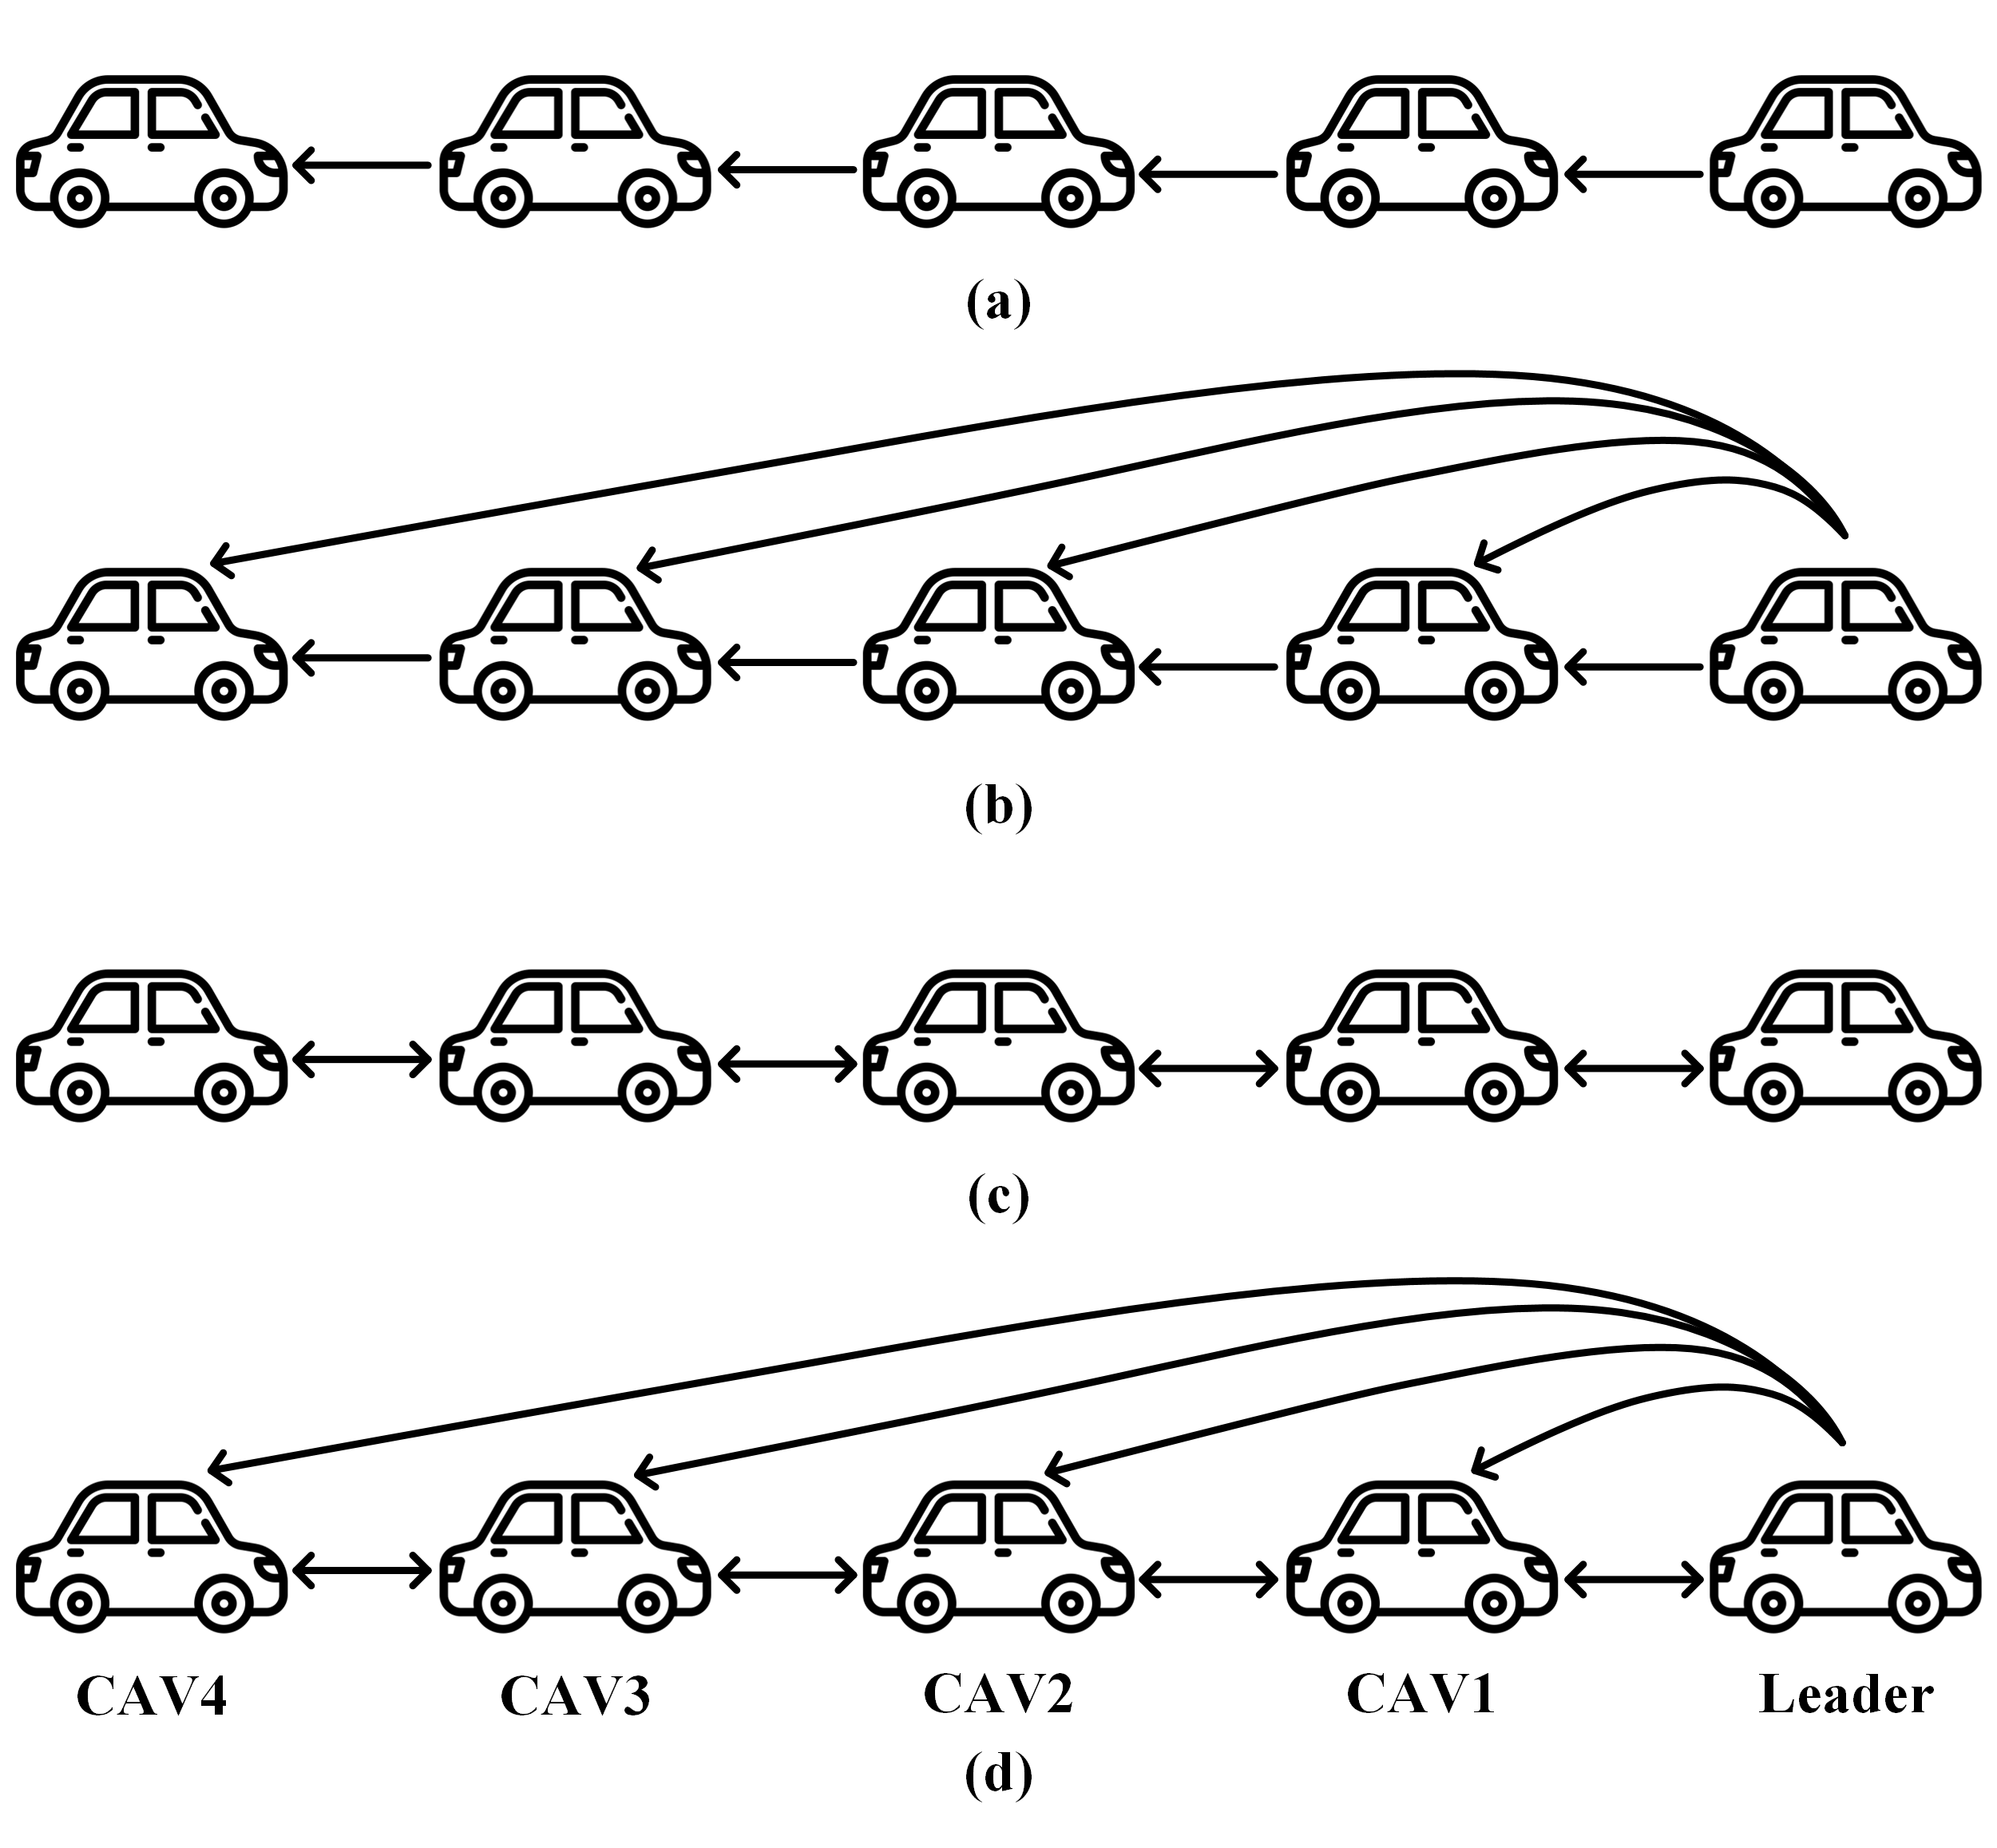
\includegraphics[width=8.5cm]{figs/fig1.png}
  \caption{~The schematic of the CAV platoon with typical IFTs, where arrows indicate the direction of information transmission, with unidirectional arrows representing one-way communication and bidirectional arrows representing two-way communication: (a) Predecessor-Follower (PF); (b) Predecessor-Leader-Follower (PLF); (c) Bi-Directional (BD); and (d) Bi-Directional-Leader (BDL).}
  \label{fig1}
\end{figure}

In this scenario, a platoon of $n$ CAVs is traveling along a single lane, and the intra-vehicle communication is carried out in accordance with the IFT protocol. Fig.\ref{fig1} illustrates the schematic of the CAV platoon with four typical IFTs, where arrows indicate the direction of information transmission, with unidirectional arrows representing one-way communication and bidirectional arrows representing two-way communication: (a) Predecessor-Follower (PF), (b) Predecessor-Leader-Follower (PLF), (c) Bi-Directional (BD), and (d) Bi-Directional-Leader (BDL). By treating the vehicles in the platoon as nodes and the intervehicle communication as edges, a weighted directed graph $\mathcal{G}=\left\{\mathcal{V},\mathcal{E},\mathcal{A}\right\}$ models the information flow topology (IFT) among the platoon. Within the digraph $\mathcal{G}$, $\mathcal{V} = \left\{ {1,2, \cdots ,n} \right\}$ denotes the nodes set and $\mathcal{E} \subseteq \mathcal{V} \times \mathcal{V} $ represents edges set. Besides, $\mathcal{A}$ is the weighted adjacent matrix with nonnegative elements defined as $\mathcal{A} = {[{a_{ij}}]_{n \times n}}$ with ${a_{ii}} = 0$ which denotes that the self-edge $\left( {i,i} \right)$ is forbidden except as noted. Moreover, the edge $\left( {i,j} \right)$ in $\mathcal{E}$ signifies the communication between vehicle $i$ and vehicle $j$ associated with weighted ${a_{ij}}$. Defining the degree matrix of $\mathcal{G}$ as $\mathcal{D} = diag\left\{ {{d_1},{d_2}, \cdots ,{d_n}} \right\}$, with ${d_i} = \sum\limits_{j \in \mathcal{V}} {{a_{ij}}}$. Within the time duration, the longitudinal position, speed, acceleration, and jerk of vehicle $i \in \mathcal{V}$ at time $t$ are denoted as $p_i\left(t\right)$, $v_i\left(t\right)={\dot{p}}_i\left(t\right)$, $a_i\left(t\right)={\ddot{p}}_i\left(t\right)$, and ${\dot{a}}_i\left(t\right)={\dddot{p}}_i\left(t\right) \in \mathbb{R}$, respectively. Via intra-vehicle communication (e.g., C-V2X according to the meeting report from the Federal Communications Commission \citep{popeo2020federal}), all vehicles within the platoon exchange state information, such as absolute position, velocity, and acceleration, with their neighboring vehicles in accordance with the IFT protocol. It is assumed that each CAV is equipped with the following components: (i) an on-board radar for detecting potential collisions by measuring the gap distance between consecutive vehicles, (ii) a GPS sensor for obtaining the longitudinal position, (iii) a wireless on-board unit that enables communication of relevant information with proximal vehicles via C-V2X communication \citep{VerizonNorth2020}, (iv) an upper-level controller that calculates the desired longitudinal acceleration based on the obtained parameters, and (v) a lower-level controller that determines the throttle and brake actuator inputs to follow the desired acceleration. This assumption is justifiable, as the sensing, communication, and actuation units listed above are standard features in modern CAVs and hence do not require any additional modifications to the existing vehicle configuration. It should be noted that the information obtained by the on-board radar regarding the surrounding environment only serves as a validation check in the event of communication unavailability or failure. This is because communication-based exchange of information is more efficient and provides more accurate data, rendering the use of radar as a supplementary measure rather than a primary source of information.


\subsection{Vehicle longitudinal dynamic Modeling}
\label{Section 3.1}

The longitudinal dynamics of vehicle $i$ can be mathematically formulated by accounting for various resistance forces influenced by the engine, throttle and brake actuators, drive train, transmission, and torque converter. The resulting model, based on the fundamental principles of Newton's second law, can be represented by the following equation:
\begin{equation}
  m_ia_i(t)=f_i^e(t)-f_i^g(t)-f_i^w(t)-f_i^r(t),
  \label{eq1}
\end{equation}
where $m_i$ stands for the unknown mass of vehicle $i$; $f_i^e(t)$ is the desired engine force acting on the vehicle $i$; $f_i^g(t)$, $\ f_i^w(t)$, and $f_i^r(t)$ denote the gravity component parallel to the road surface, air resistance force, and rolling resistance force, respectively.

The nonlinearity of the system~(\ref{eq1}) makes it challenging to controller design challenging. Therefore, a feedback control input in Appendix A is employed to convert it into a linear form \citep{Wang2018}:
\begin{equation}
  \tau_i\dot{a_i}\left(t\right)+a_i\left(t\right)=u_i(t),
  \label{eq2}
\end{equation}
where $u_i(t)$ denotes the control input of the lower-level controller, which can be interpreted as the desired acceleration of vehicle $i$, $\tau_i$ denotes the time constant that represents the delay caused by the engine actuator.

Reformulate Equation~(\ref{eq2}), the state space equation can be represented as:
\begin{equation}
  {\dot x_i}\left( t \right) = A{x_i}\left( t \right) + B{u_i}\left( t \right),
  \label{eq3}
\end{equation}
with $A = \left[ {\begin{array}{*{20}{c}}
          0 & 1 & 0                          \\
          0 & 0 & 1                          \\
          0 & 0 & { - \frac{1}{{{\tau _i}}}}
        \end{array}} \right]$ and $B = \left[ {\begin{array}{*{20}{c}}
          0 \\
          0 \\
          {\frac{1}{{{\tau _i}}}}
        \end{array}} \right]$,\\
where ${x_i}\left( t \right) = {\left[ {\begin{array}{*{20}{c}}
          {{p_i}\left( t \right)} & {{v_i}\left( t \right)} & {{a_i}\left( t \right)}
        \end{array}} \right]^T} \in {\mathbb{R}^3}$ denotes the state vector of vehicle $i$.

Subject to limited communication, the inputs for vehicle $i$ are controlled by an appropriate decentralized coupling protocol of communication information:
\begin{equation}
  {u_i} = {u_i}\underbrace {\left( {{x_1}\left( {t - h(t)} \right), \cdots ,{x_i}\left( t \right), \cdots ,{x_n}\left( {t - h(t)} \right)} \right)}_n,
  \label{eq4}
\end{equation}
where $ h(t) $ represents the time-varying communication delay within the transmission range which is assumed to be influenced by the surrounding environment \citep{jia_enhanced_2016,Vukadinovic2018,Vu2020,Martin-Sacristan2020,Pirani2022}. And it satisfies the following constraints:
\begin{equation}
  h(t) \in \left[ {{h_m},{h_M}} \right],\quad \dot h(t) \in \left[ {{d_m},{d_M}} \right],\quad \forall t \geqslant 0,
  \label{eq5}
\end{equation}
where $ 0 \leqslant {h_m} \leqslant {h_M} $ and $ {d_m} \leqslant {d_M} \leqslant 1 $.

Assuming that CAVs adopt the Constant Time Headway (CTH) policy, where CAVs maintain a desired time headway from the reference vehicle, we can formulate the cooperative tracking problem of vehicle $i$ as follows:
\begin{equation}
  \left\{ \begin{gathered}
    \mathop {\lim }\limits_{t \to \infty } \left\| {\sum\limits_{j = 1}^n {\left| {{p_i}(t) - {p_j}(t - h(t)){\text{ + }}{h_{ij}}{v_i}(t)} \right|} } \right\| = 0 \hfill, \\
    \mathop {\lim }\limits_{t \to \infty } \left\| {\sum\limits_{j = 1}^n {\left| {{v_i}(t) - {v_j}(t - h(t))} \right|} } \right\| = 0, \hfill \\
    \mathop {\lim }\limits_{t \to \infty } \left\| {\sum\limits_{j = 1}^n {\left| {{a_i}(t) - {a_j}(t - h(t))} \right|} } \right\| = 0. \hfill \\
  \end{gathered}  \right.,\forall i = 1, \ldots ,N.
  \label{eq6}
\end{equation}
where $ {h_{ij}} =  - {h_{ji}} $ stands for the constant time headway between vehicle $i$ and vehicle $j$.

By implementing a suitable distributed control strategy, the consensus objective stated in Equation~(\ref{eq6}) can be attained. Therefore, the vehicle $i$ updates its dynamics via an onboard computation of the following decentralized coupling protocol:
\begin{equation}
  {u_i} =  - \sum\limits_{j = 1}^n {{a_{ij}}{k_{ij}}^T{{\left[ {\begin{array}{*{20}{c}}
              {{p_i}\left( t \right) - {p_j}\left( {t - h(t)} \right) + {h_{ij}}{v_i}\left( t \right)} \\ {{v_i}\left( t \right) - {v_j}\left( {t - h(t)} \right)} \\ {{a_i}\left( t \right) - {a_j}\left( {t - h(t)} \right)}
            \end{array}} \right]}}},
  \label{eq7}
\end{equation}
where $ {a_{ij}} $ denotes the weight of edge $ \left( {i,j} \right) $ and $ {a_{ij}} = 0 $ if there is no edge $ \left( {i,j} \right) $; $ {k_{ij}} = {\left[ {\begin{array}{*{20}{c}}
          {{\alpha _{ij}}} & {{\beta _{ij}}} & {{\gamma _{ij}}}
        \end{array}} \right]^T} \in {\mathbb{R}^{3 \times 1}} $ presents the feedback control gain vector, with $ {\alpha _{ij}} $, $ {\beta _{ij}} $, and $ {\gamma _{ij}} $ denoting the control gain of spacing, speed, and acceleration error, respectively.


\subsection{CAV platoon Modeling}
\label{Section 3.2}

To achieve consensus of systems~(\ref{eq3}) and~(\ref{eq4}) under the influence of the coupling protocol~(\ref{eq7}), it is necessary to reformulate the decentralized coupling protocol~(\ref{eq7}) as follows:
\begin{equation}
  {u_i} =  - \sum\limits_{j = 1}^n {{a_{ij}}{k_{ij}}^T\left[ {{\psi _{ij}}{x_i}(t) - {x_j}(t - h(t))} \right]},
  \label{eq10}
\end{equation}
where $ {\psi _{ij}}{\text{ = }}\left[ {\begin{array}{*{20}{c}}
          1  & {{h_{ij}}} & {} \\
          {} & 1          & {} \\
          {} & {}         & 1
        \end{array}} \right] $ denotes the relationship between the states based on the CTH policy.

Therefore, the dynamics of the error system can be presented as:
\begin{equation}
  \left\{ \begin{gathered}
    {{\dot {\tilde p}}_i} = {{\tilde v}_i}, \hfill \\
    {{\dot {\tilde v}}_i} = {{\tilde a}_i}, \hfill\\
    {{\dot {\tilde a}}_i} =  - \frac{1}{\tau }{{\tilde a}_i} - \frac{1}{\tau }\sum\limits_{j = 1}^n {{a_{ij}}{k_{ij}}^T\left( {{\psi _{ij}}{x_i}(t) - {x_j}(t - h(t))} \right)}.  \hfill \\
  \end{gathered}  \right.
  \label{eq11}
\end{equation}

From Equation~(\ref{eq11}), the dynamics of the closed-loop vehicular network can be reformulated using supermatrices, resulting in a more concise representation:
\begin{equation}
  {\dot x_i}\left( t \right) = A{x_i}\left( t \right) - B\sum\limits_{j = 1}^n {{a_{ij}}{k_{ij}}^T\left( {{\psi _{ij}}{x_i}(t) - {x_j}(t - h(t))} \right)}.
  \label{eq12}
\end{equation}

\begin{theorem}
  \label{theorem3}
  The CAV platoon under CTH policy with time-varying communication delay can be modeled as a linear time-invariant state time-varying delay system:
  \begin{equation}
    \left\{ \begin{gathered}
      \dot X\left( t \right) = \Psi X\left( t \right) + {\Psi _d}X(t - h(t)),\quad \forall t \geqslant 0 \hfill \\
      X\left( t \right) = \phi \left( t \right),\quad \quad \quad \quad \quad \quad \quad \forall t \in \left[ { - h,0} \right] \hfill \\
    \end{gathered}  \right.
    \label{eq13}
  \end{equation}
  with
  
  \begin{equation}
    \left\{ {\begin{array}{*{20}{l}}
          {\Psi  = {A^*} - {B^*}\mathcal{F}{E_1} \in {\mathbb{R}^{3n \times 3n}}}                                         \\
          \begin{gathered}
            {\Psi _d} = {B^*}\mathcal{J}{E_2} \in {\mathbb{R}^{3n \times 3n}} \hfill \\
            {A^*} = {I_n} \otimes A \in {\mathbb{R}^{3n \times 3n}} \hfill \\
          \end{gathered}                                                                                      \\
          {{B^*} = {I_n} \otimes B \in {\mathbb{R}^{3n \times n}}}                                                        \\
          \begin{gathered}
            \mathcal{K} = {[{k_{ij}}^T]_{n \times n}} \hfill \\
            \mathcal{H} = \mathcal{A} \circ \mathcal{K} = {[{a_{ij}} \otimes {k_{ij}}^T]_{N \times N}} \in {\mathbb{R}^{n \times 3n}} \hfill \\
            \mathcal{J} = diag\underbrace {\left\{ {{\mathcal{D}_1},{\mathcal{D}_2}, \cdots ,{\mathcal{D}_N}} \right\}}_n \in {\mathbb{R}^{n \times 3{n^2}}} \hfill \\
            {\mathcal{D}_i} = \underbrace {\left[ {{a_{i1}}{k_{i1}}^T,{a_{i2}}{k_{i2}}^T, \cdots ,{a_{in}}{k_{in}}^T} \right]}_n \in {\mathbb{R}^{1 \times 3n}},\forall i \in \mathcal{V} \hfill \\
            \mathcal{F} = diag\underbrace {\left\{ {{\mathcal{H}_1},{\mathcal{H}_2}, \cdots ,{\mathcal{H}_N}} \right\}}_n \in {\mathbb{R}^{n \times 3{n^2}}} \hfill \\
            % {\mathcal{H}_i} = \underbrace {\left[ {{a_{i1}}{k_{i1}}^T{\psi _{i1}},{a_{i2}}{k_{i2}}^T{\psi _{i2}}, \cdots ,{a_{in}}{k_{in}}^T{\psi _{in}}} \right]}_n \in {\mathbb{R}^{1 \times 3n}},\forall i \in \mathcal{V} \hfill \\
            {\mathcal{H}_i} = {\mathcal{D}_i} \circ \underbrace {\left[ {{\psi _{i1}},{\psi _{i2}}, \cdots ,{\psi _{in}}} \right]}_n \in {\mathbb{R}^{1 \times 3n}},\forall i \in \mathcal{V} \hfill \\
          \end{gathered}                                                                                      \\
          {{E_1} = diag\underbrace {\left\{ {{I_1},{I_1}, \cdots ,{I_1}} \right\}}_n \in {\mathbb{R}^{3{n^2} \times 3n}}} \\
          {{E_2} = {{\underbrace {\left[ {\begin{array}{*{20}{c}}
                            {{I_2}^T} & \cdots & {{I_2}^T}
                          \end{array}} \right]}_n}^T} \in {\mathbb{R}^{3{n^2} \times 3n}}} \\
          {{I_1} = {{\underbrace {\left[ {\begin{array}{*{20}{c}}
                            {{I_3}^T} & \cdots & {{I_3}^T}
                          \end{array}} \right]}_n}^T} \in {\mathbb{R}^{3n \times 3}}}      \\
          {{I_2} = {I_{3n}} \in {\mathbb{R}^{3n \times 3n}}}                                                              \\
          {{I_3} = {I_3} \in {\mathbb{R}^{3 \times 3}}}
        \end{array}} \right.
    \label{eq14}
  \end{equation}
  where $ X\left( t \right) = {\left[ {\begin{array}{*{20}{c}}
            {{x_1}^T} & \cdots & {{x_n}^T}
          \end{array}} \right]^T} \in {\mathbb{R}^{3n}} $ stands for the error state vector of the closed-loop vehicular network; $ \phi  $ is the initial conditions; $ \Psi$ and $ {\Psi _d} $ are constant matrix according to their definitions.

\end{theorem}


\section{Stability analyses}
\label{Section 4}

The Lyapunov-Krasovskii Stability Theorem is a commonly used method for analyzing stability in state delay systems. This approach is an extension of the Second Lyapunov method, which is specifically designed for stability analysis \citep{Gu2003}. It involves the use of "energy" functionals that are both positive definite and monotonically decreasing along the system trajectories. The statement of the Lyapunov-Krasovskii Theorem is presented below:
\begin{lemma}
  \label{lemma3}
  (Lyapunov-Krasovskii Stability Theorem \citep{Gu2009}). Given system (\ref{eq13}), suppose that $f$ maps $\mathbb{R} \times  $(bounded sets in ${\mathbb{R}^n} \times \mathcal{C} $) into bounded sets in ${\mathbb{R}^n} $, and that $u,v,w:{\mathbb{R}_ + } \to {\mathbb{R}_ + } $ are continuous nondecreasing functions, where additionally $u(s) $ and $v(s) $ are positive for $s > 0 $, and $u(0) = v(0) = 0 $. If there exists a functional $V:\mathbb{R} \times {\mathbb{R}^n} \times \mathcal{C} \to \mathbb{R} $ such that
  \begin{equation}
    \left\{ \begin{gathered}
      u(|\phi \left( 0 \right)|) \leqslant V(t,\phi ) \leqslant v(|\phi {|_h}) \hfill, \\
      \dot V(t,\phi ) \leqslant  - w(|\phi \left( 0 \right)|). \hfill \\
    \end{gathered}  \right.
    \label{eq15}
  \end{equation}
  Then the trivial solution of the system (\ref{eq13}) is uniformly stable. If $w(s) > 0 $ for $s > 0 $, then it is uniformly asymptotically stable. If, in addition, $\mathop {\lim }\limits_{s \to \infty } u(s) =  + \infty  $, then it is globally uniformly asymptotically stable. Such a functional $V $ is called a Lyapunov-Krasovskii functional (LKF).
\end{lemma}

Moreover, integral inequalities provide significant assistance in the study of lower bounds of quadratic function integrals for the stability analysis of state-delayed systems \citep{martyniuk_integral_1979,zhang_stability_2016,li_uniform_2021}. Among them, Wirtinger Integral inequalities are considered to be effective and less conservative \citep{saravanan_finite-time_2021,suresh_robust_2021}. Wirtinger Integral inequalities are a series of integral inequalities that employ the integral of a function to estimate the integral of its derivative function. The Wirtinger Integral inequality is stated as follows:
\begin{lemma}
  \label{lemma1}
  (Wirtinger Integral Inequality \citep{park_stability_2015}). Given a positive definite $n \times n$ matrix $R$, the following inequality holds for any $z \in \mathcal{C}\left( {\left[ { - h,0} \right],{\mathbb{R}^n}} \right)$ that satisfies $z(-h) = z(0) = 0$:
  \begin{equation}
    \int_{ - h}^0 {{{\dot z}^T}} (u)R\dot z(u){\text{d}}u \geqslant \frac{{{\pi ^2}}}{{{h^2}}}\int_{ - h}^0 {{z^T}} (u)Rz(u){\text{d}}u.
    \label{eqlemma1}
  \end{equation}
\end{lemma}

Although the Jensen inequality \citep{Gu2003} is commonly employed in research to establish lower bounds of quadratic function integrals, its inherent conservatism can lead to less precise results. To obtain more accurate lower bounds, the Wirtinger Integral Inequality can be utilized, as highlighted in Remark~\ref{remarkXX}.

Additionally, we present another useful lemma that is motivated by the concept of reciprocally convex combination:
\begin{lemma}
  \label{lemma2}
  (\citep{park_reciprocally_2011}) Let $n$ and $m$ be positive integers, $\alpha \in (0,1)$ be a scalar, $R \succ 0$ be a given $n \times n$ matrix, and $W_1$ and $W_2$ be two $n \times m$ matrices in $\mathbb{R}^{n \times m}$. The function $\Theta (\alpha ,R)$ is defined for all vectors $\xi$ in $\mathbb{R}^m$ as follows:
  \begin{equation}
    \Theta (\alpha ,R) = \frac{1}{\alpha }{\xi ^T}W_1^TR{W_1}\xi  + \frac{1}{{1 - \alpha }}{\xi ^T}W_2^TR{W_2}\xi.
    \label{eqlemma21}
  \end{equation}
  Then, if there exists a matrix $X$ in $ {\mathbb{R}^{n \times n}} $ such that $ \left[ {\begin{array}{*{20}{l}}
            R & X \\
            * & R
          \end{array}} \right] \succ 0 $, then the following inequality holds:
  \begin{equation}
    \mathop {\min }\limits_{\alpha  \in (0,1)} \Theta (\alpha ,R) \geqslant {\left[ {\begin{array}{*{20}{l}}
              {{W_1}\xi } \\
              {{W_2}\xi }
            \end{array}} \right]^T}\left[ {\begin{array}{*{20}{c}}
            R & X \\
            * & R
          \end{array}} \right]\left[ {\begin{array}{*{20}{l}}
            {{W_1}\xi } \\
            {{W_2}\xi }
          \end{array}} \right].
    \label{eqlemma22}
  \end{equation}
\end{lemma}


Lemma~\ref{lemma3} aims to establish a positive definite functional whose time derivative is negative definite along the trajectories of the system (\ref{eq13}). This forms the core idea behind the lemma. In the context of the stability analysis of such systems using LKF, several types of functionals have been provided in the literature. Among them, an integral quadratic term is one of the most relevant components of LKF \citep{pepe_lyapunovkrasovskii_2006}:
\begin{equation}
  V\left( {{X_t}} \right) = \int_{0 - h}^0 {\int_\theta ^0 {{{\dot X}_t}^T(s)R{{\dot X}_t}(s){\text{d}}s\;{\text{d}}\theta } },
  \label{eq16}
\end{equation}
where $ {\dot X_t}(s) = {\dot X}(t + s) $ denotes the state of the state delay system, $ R \succ 0 $ and $ h > 0 $.

The positivity of LKF (\ref{eq16}) is ensured by $ R \succ 0 $. Then another that needs to be clarified is the negation of its derivative. Differentiating this term with respect to the time $t$, we get:
\begin{equation}
  \dot V\left( {{X_t}} \right) = h{\dot X^T}(t)R\dot X(t) - \int_{ - h}^0 {{{\dot X}^T}} (s)R\dot X(s){\text{d}}s.
  \label{eq17}
\end{equation}

To transform Equation (\ref{eq17}) into a suitable LMI framework, an over-approximation process of the integral terms is required as they cannot be readily converted using the quadratic formulation discussed previously. Consequently, the current task is to derive a new lower bound of integral quadratic terms in the following format:
\begin{equation}
  F(\omega ) = \int_{ - h}^0 {{\omega ^T}} (s)R\omega (s){\text{d}}s,
  \label{eq18}
\end{equation}
where $ \omega  $ is a continuous function from $ [a,b] \to {\mathbb{R}^n} $ and consequently integrable.

\begin{corollary}
  \label{coro4}
  Given a positive definite matrix $ R $, the following inequality holds for all continuous functions $ \omega : [a,b] \to {\mathbb{R}^n} $:
  \begin{equation}
    F(\omega ) \geqslant \frac{1}{h}{\left( {\int_{ - h}^0 {\omega (u){\text{d}}u} } \right)^T}R\left( {\int_{ - h}^0 {\omega (u){\text{d}}u} } \right) + \frac{3}{h}{\Omega ^T}R\Omega,
    \label{eq19}
  \end{equation}
  where $ \Omega  = \int_{ - h}^0 {\omega (s){\text{d}}s}  - \frac{2}{h}\int_{ - h}^0 {\int_{ - h}^s {\omega (r){\text{d}}r\;{\text{d}}s} }  $.
\end{corollary}

\begin{IEEEproof}
  We first construct the function $z$ for all $ u \in [a,b] $ as:
  \begin{equation}
    z(u) = \int_{ - h}^u {\omega (s){\text{d}}s}  - \frac{{u + h}}{h}\int_{ - h}^0 {\omega (s){\text{d}}s}  - \frac{{( - u)(u + h)}}{{{h^2}}}\Theta,
    \label{eq20}
  \end{equation}
  where $ \Theta  $ is a constant vector of $ {\mathbb{R}^n} $ to be defined. Moreover, the function $z\left(u\right)$~(\ref{eq20}) satisfies the constrains of Lemma~\ref{lemma1}, that is $ z(0) = z( - h) = 0 $ according to its definition.

Then, calculating the left-hand-side of the inequality mentioned in Lemma~\ref{lemma1} yields:
\begin{equation}
     \begin{gathered}
     \int_{ - h}^0 {{{\dot z}^T}(u)R\dot z(u){\text{d}}u}  =   2\int_{ - h}^0 {\left( {\frac{{( - h - 2u)}}{{{h^2}}}} \right){\text{d}}u} {\Theta ^T}R\left( {\int_{ - h}^0 {\omega (u){\text{d}}u} } \right) \hfill \\
    + \int_{ - h}^0 {{{\left( {\frac{{(h + 2u)}}{{{h^2}}}} \right)}^2}{\text{d}}u{\Theta ^T}R\Theta } \; - 2{\Theta ^T}R\int_{ - h}^0 {\left( {\frac{{ - h - 2u}}{{{h^2}}}} \right)\omega (u){\text{d}}u}  \hfill \\
     +\int_{ - h}^0 {{\omega ^T}(u)R\omega (u){\text{d}}u}  - \frac{1}{h}{\left( {\int_{ - h}^0 {\omega (u){\text{d}}u} } \right)^T}R\left( {\int_{ - h}^0 {\omega (u){\text{d}}u} } \right). \hfill \\
     \end{gathered}
     \label{eq21}
\end{equation}
 % \begin{equation}
  %  \begin{gathered}
  %    \int_{ - h}^0 {{{\dot z}^T}(u)R\dot z(u){\text{d}}u}  = \int_{ - h}^0 {{\omega ^T}(u)R\omega (u){\text{d}}u}  - \frac{1}{h}{\left( {\int_{ - h}^0 {\omega (u){\text{d}}u} } \right)^T}R\left( {\int_{ - h}^0 {\omega (u){\text{d}}u} } \right) \hfill \\
  %    \quad \quad \quad \quad \quad \quad \quad  + \int_{ - h}^0 {{{\left( {\frac{{(h + 2u)}}{{{h^2}}}} \right)}^2}{\text{d}}u{\Theta ^T}R\Theta } \; - 2{\Theta ^T}R\int_{ - h}^0 {\left( {\frac{{ - h - 2u}}{{{h^2}}}} \right)\omega (u){\text{d}}u}  \hfill \\
  %    \quad \quad \quad \quad \quad \quad \quad  + 2\int_{ - h}^0 {\left( {\frac{{( - h - 2u)}}{{{h^2}}}} \right){\text{d}}u} {\Theta ^T}R\left( {\int_{ - h}^0 {\omega (u){\text{d}}u} } \right). \hfill \\
  %  \end{gathered}
 %   \label{eq21}
  %\end{equation}

  Substituting $ \int_{ - h}^0 { - h - 2u{\text{d}}u}  = 0 $ and applying integration by parts, Equation~(\ref{eq21}) can be simplified as follows:
  \begin{equation}
    \begin{aligned}
      &\int_{ - h}^0 {{{\dot z}^T}(u)R\dot z(u){\text{d}}u}  = \int_{ - h}^0 {{\omega ^T}(u)R\omega (u){\text{d}}u} \\
       &- \frac{1}{h}{\left( {\int_{ - h}^0 {\omega (u){\text{d}}u} } \right)^T}R\left( {\int_{ - h}^0 {\omega (u){\text{d}}u} } \right) \hfill \\
      &- \frac{3}{{(b - a)}}{\Omega ^T}R\Omega  + \frac{1}{{3(b - a)}}{(\Theta  + 3\Omega )^T}R(\Theta  + 3\Omega ). \hfill \\
    \end{aligned}
    \label{eq22}
  \end{equation}

  Substituting $ \int_{ - h}^0 z (u){\text{d}}u =  - \frac{h}{6}(\Theta  + 3\Omega ) $ and applying Lemma~\ref{lemma1}, it yields:
  \begin{equation}
    \begin{gathered}
      F(\omega ) \geqslant \frac{1}{h}{\left( {\int_{ - h}^0 {\omega (u){\text{d}}u} } \right)^T}R\left( {\int_{ - h}^0 {\omega (u){\text{d}}u} } \right) + h{\Omega ^T}R\Omega  \hfill \\
      \quad \quad \quad \quad \quad \quad \quad \quad  + \frac{{{\pi ^2} - 12}}{{36h}}{(\Theta  + 3\Omega )^T}R(\Theta  + 3\Omega ). \hfill \\
    \end{gathered}
    \label{eq23}
  \end{equation}

  Given that $ \frac{{{\pi ^2} - 12}}{{36h}} > 0 $, the third term on the right-hand side of the inequality~(\ref{eq23}) is positive definite, regardless of the selection of $ \Theta $. Moreover, the inequality is equivalent to equality if and only if $ \Theta  =  - 3\Omega  $. Furthermore, the definite positiveness of $ F(\omega ) $ is guaranteed by $ R \succ 0 $. 
  
\textbf{This concludes the proof.}

\end{IEEEproof}

\begin{remark}
  \label{remarkXX}
  Note that the first term to the right of Inequality~(\ref{eq19}) is Jensen inequality \citep{Gu2003}. Since the second term is definite positive, the lower bound of the integral is evidently higher than the result obtained through Jensen inequality. Therefore, with Wirtinger-Based Integral Inequality, more accurate stability conditions can be obtained.
\end{remark}


According to Inequality~(\ref{eq17}), another lower bound needed to be determined is the case of $ F(\dot \omega ) $. Therefore, Corollary~\ref{coro4} is rewritten as follows:
\begin{corollary}
  \label{coro5}
  Given a positive definite matrix $R$, all continuously differentiable functions $\omega : [a,b] \to \mathbb{R}^n$ satisfy the subsequent inequality:
  \begin{equation}
    \label{eq24}
    F(\dot \omega ) \geqslant {\text{ }}\frac{1}{h}{(\omega (0) - \omega ( - h))^T}R(\omega (0) - \omega ( - h)) + \frac{3}{h}{\tilde \Omega ^T}R\tilde \Omega,
  \end{equation}
  where $ \tilde \Omega  = \omega (0) + \omega ( - h) - \frac{2}{h}\int_a^b \omega  (u){\text{d}}u $.
\end{corollary}

The subsequent stability theorem is presented below:
\begin{theorem}
  \label{theorem6}
  Assuming the existence of $ P \in \mathbb{S}_{3n}^ + $, three matrices $ S, R, Q \in \mathbb{S}n^ + $, and $ X \in \mathbb{S}{2n} $, the ensuing LMIs hold for $ h = { {h_m},{h_M}} $ and $ \dot h = { {d_m},{d_M}} $.
  \begin{equation}
    \label{eq25}
    {\Phi _1}(h,\dot h) = {\Phi _0}(h,\dot h) - \frac{1}{{{h_M}}}{\Gamma ^T}{\Phi _2}\Gamma  \prec 0,
  \end{equation}
  \begin{equation}
    \label{eq26}
    {\Phi _2} = \left[ {\begin{array}{*{20}{c}}
            {\tilde R} & X          \\
            *          & {\tilde R}
          \end{array}} \right] \succ 0,
  \end{equation}
  where
  \begin{itemize}
    \item[]
      $ {\Phi _0}(h,\dot h) = \operatorname{He} \left( {G_1^T(h)P{G_0}(\dot h)} \right) + \hat S + \hat Q(\dot h) + {h_M}G_0^T(\dot h)\hat R{G_0}(\dot h) $;                     \\
      $ \Gamma  = {\left[ {\begin{array}{*{20}{c}}
                {K_1^T} & {K_2^T}
              \end{array}} \right]^T} $;\\
      $ {K_1} = \left[ {\begin{array}{*{20}{c}}
                I & { - I} & 0 & 0       & 0 \\
                I & I      & 0 & { - 2I} & 0
              \end{array}} \right] $;\\
      $ {K_2} = \left[ {\begin{array}{*{20}{c}}
                0 & I & { - I} & 0 & 0       \\
                0 & I & I      & 0 & { - 2I}
              \end{array}} \right] $;\\
      $ \hat Q(\dot h) = \operatorname{diag} \left( {Q, - (1 - \dot h)Q,{0_{3n}}} \right) $;\\
      $ \hat S = \operatorname{diag} \left( {S,0, - S,{0_{2n}}} \right) $;\\
      $ \hat R = \operatorname{diag} \left( {R,{0_{3n}}} \right) $;\\
      $ \tilde R = \operatorname{diag} (R,3R) $;\\
      $ {G_0}(\dot h) = \left[ {\begin{array}{*{20}{c}}
                \Psi & {{\Psi _d}}        & 0      & 0 & 0 \\
                I    & { - (1 - \dot h)I} & 0      & 0 & 0 \\
                0    & {(1 - \dot h)I}    & { - I} & 0 & 0
              \end{array}} \right] $;\\
      $ {G_1}(h) = \left[ {\begin{array}{*{20}{c}}
                I & 0 & 0 & 0    & 0                             \\
                0 & 0 & 0 & {hI} & 0                             \\
                0 & 0 & 0 & 0    & {\left( {{h_M} - h} \right)I}
              \end{array}} \right] $.\\
  \end{itemize}
  Then the system (\ref{eq13}) is asymptotically stable for all delay function $h$ satisfying (\ref{eq5}).

\end{theorem}

\begin{IEEEproof}
  We first construct the LKF as:
  \begin{equation}
    \label{eq27}
    \begin{gathered}
      V\left( {h,{x_t},{{\dot x}_t}} \right) = {{\tilde x}^T}(t)P\tilde x(t) + \int_{ - h(t)}^0 {{x^T}} (s)Qx(s){\text{d}}s \hfill \\
      \quad \quad \quad \quad \quad  + \int_{ - {h_M}}^0 {{x^T}} (s)Sx(s){\text{d}}s + \int_{ - {h_M}}^0 {\int_\theta ^0 {{{\dot x}^T}(s)R\dot x(s){\text{d}}s\;{\text{d}}\theta } },  \hfill \\
    \end{gathered}
  \end{equation}
  where $ \tilde x(t) = {\left[ {{x^T}(t),\quad \int_{ - h(t)}^0 {{x^T}} (s){\text{d}}s,\quad \int_{ - {h_M}}^{ - h(t)} {{x^T}} (s){\text{d}}s} \right]^T} $.

  The positivity of LKF (\ref{eq27}) is guaranteed by $ P \succ 0 $, $ Q \succ 0 $, $ S \succ 0 $, and $ R \succ 0 $. Consequently, the negation of its derivative needs to be elucidated. Upon differentiating the functional (\ref{eq17}) along the trajectories of (\ref{eq13}), we obtain:
  \begin{equation}
    \label{eq28}
    \dot V\left( {h,{x_t},{{\dot x}_t}} \right) = \zeta _1^T(t){\Phi _0}(h,\dot h){\zeta _1}(t) - \int_{ - {h_M}}^0 {{{\dot x}^T}} (s)R\dot x(s){\text{d}}s,
  \end{equation}
  where $ {\zeta _1}(t) = \left[ {\begin{array}{*{20}{c}}
            {x(t)}                                              \\
            {x(t - h(t))}                                       \\
            {x\left( {t - {h_M}} \right)}                       \\
            {\frac{1}{{h(t)}}\int_{ - h(t)}^0 x (s){\text{d}}s} \\
            {\frac{1}{{{h_M} - h(t)}}\int_{ - {h_M}}^{ - h(t)} x (s){\text{d}}s}
          \end{array}} \right] $.

  Notice the Equation (\ref{eq28}) can be obtained by substituting $ \tilde x(t) = {G_1}(h){\zeta _1}(t) $ and $ \dot {\tilde x}(t) = {G_0}(\dot h){\zeta _1}(t) $ into the partial differential of Equation (\ref{eq27}).

  Then split the integral interval of Equation (\ref{eq28}) into two parts: $ [ - {h_M}, - h(t)] $ and $ [ - {h_M},0] $, and apply Corollary~\ref{coro5} respectively to get:
  \begin{equation}
    \begin{aligned}
    \label{eq29}
    - &\int_{t - {h_M}}^t {{{\dot x}^T}} (s)R\dot x(s){\text{d}}s \leqslant  \\
     &- \zeta _1^T(t)\left( {\frac{1}{{h(t)}}K_1^T\tilde R{K_1}} \right.\left. { + \frac{1}{{{h_M} - h(t)}}K_2^T\tilde R{K_2}} \right){\zeta _1}(t).
    \end{aligned}
  \end{equation}

  Given the constraint of Lemma~\ref{lemma2}, assuming the existence of $X$ such that $ {\Phi _2} \succ 0 $, we can conclude that the ensuing inequality holds true:
  \begin{equation}
    \label{eq30}
    - \int_{t - {h_M}}^t {{{\dot x}^T}} (s)R\dot x(s){\text{d}}s \leqslant  - \frac{1}{{{h_M}}}\zeta _1^T(t){\Gamma ^T}{\Phi _2}\Gamma {\zeta _1}(t),
  \end{equation}

  Substituting Inequality~(\ref{eq30}) into Equation~(\ref{eq28}), it yields:
  \begin{equation}
    \label{eq31}
    \begin{gathered}
      \dot V\left( {h,{x_t},{{\dot x}_t}} \right) \leqslant \zeta _1^T(t){\Phi _0}(h,\dot h){\zeta _1}(t) - \frac{1}{{{h_M}}}\zeta _1^T(t){\Gamma ^T}{\Phi _2}\Gamma {\zeta _1}(t) \hfill \\
      \quad \quad \quad \quad \quad  = \zeta _1^T(t)\left( {{\Phi _0}(h,\dot h) - \frac{1}{{{h_M}}}{\Gamma ^T}{\Phi _2}\Gamma } \right){\zeta _1}(t) \hfill \\
      \quad \quad \quad \quad \quad {\text{ = }}\zeta _1^T(t){\Phi _1}(h,\dot h){\zeta _1}(t). \hfill \\
    \end{gathered}
  \end{equation}

Equation~(\ref{eq31}) ensures the negative definiteness of $\dot V\left( {h,{x_t},{{\dot x}_t}} \right)$ by imposing the constraint ${\Phi _1}(h,\dot h) \prec 0$. It is important to note that the matrix ${\Phi _1}(h,\dot h)$ is affine and therefore convex with respect to $h(t)$ and $\dot h(t)$. Consequently, to guarantee ${\Phi _1}(h,\dot h) \prec 0$, it is necessary and sufficient to confine it to the vertices of the intervals $\left[ {0,{h_M}} \right] \times \left[ {{d_m},{d_M}} \right]$.

To sum up, the negative definiteness of $\dot V\left( {h,{x_t},{{\dot x}_t}} \right)$ is ensured if a matrix $X$ exists such that ${\Phi _2} \succ 0$ and ${\Phi _1}(h,\dot h) \prec 0$ holds for all $(h,\dot h) \in \left[ {0,{h_M}} \right] \times \left[ {{d_m},{d_M}} \right]$. 

\textbf{This completes the proof.}

\end{IEEEproof}


\begin{remark}
  \label{remarkdiff}
  The key idea of the Lyapunov-Krasovskii Stability Theorem is that it is not necessary to establish the negative definiteness of $V\left(t,X\left(t\right)\right)$ along all system trajectories. Rather, it is sufficient to ensure its negative definiteness for solutions that tend to move away from the vicinity of $V\left(t,X\left(t\right)\right)\le c$ of the equilibrium. Appendix B offers an in-depth theoretical analysis of this concept.
\end{remark}

\begin{remark}
  \label{remark7}
  The code to construct the LMIs in Theorem~\ref{theorem6} is available on GitHub for future research purposes. The associated URL can be found in Appendix C for additional reference.
\end{remark}

\section{Numerical analyses}
\label{Section 5}
In this section, a thorough examination of numerical simulations and analyses is conducted to highlight the primary outcomes. The investigation focuses on the tracking performance and safety conditions of a CAV platoon employing the PLF, with various feedback control gains. Moreover, the tracking performances of the CAV platoon using the remaining three IFTs are also explored.

\subsection{Numerical Setup}
\label{Section 5.1}
For a thorough performance evaluation, a CAV platoon consisting of 5 interconnected CAVs utilizing the PLF, as depicted in Fig.\ref{fig1} (b), is considered. The Leader CAV follows a specified speed profile, while the other CAVs operate under the control strategy. It should be noted that each CAV in the platoon communicates solely with its neighbors in the PLF. Furthermore, control parameters must be set in accordance with the specific control strategy employed. For additional analysis, parameters for both network and traffic simulations are established in Table~\ref{table1}, maintaining simplicity without sacrificing generality. It is important to highlight that the weights of the weighted adjacency matrix are set to $ {a_{ij}} = \frac{1}{{{d_i}}},\forall (i,j) \in \mathcal{E} $, indicating that the information from each neighbor has an equal impact on the control decision. Regarding the time-varying delay, the time-varying equation is provided below in the form of the Bessel function of the first kind \citep{liang2017spectrum,soret2010capacity,vicario2006analytical}. The time-varying curve, shown in Fig.\ref{fig2}, satisfies the constraint in Equation (\ref{eq5}):
\begin{equation}
  \label{eq51}
  {J_{40}}(t) = \sum\limits_{k = 0}^\infty  {\frac{{{{( - 1)}^k}}}{{k!(k + 40)!}}} {\left( {\frac{{t{\text{ + }}30}}{2}} \right)^{2k + 40}},\quad t \geqslant 0.
\end{equation}


\begin{figure}
  \centering

  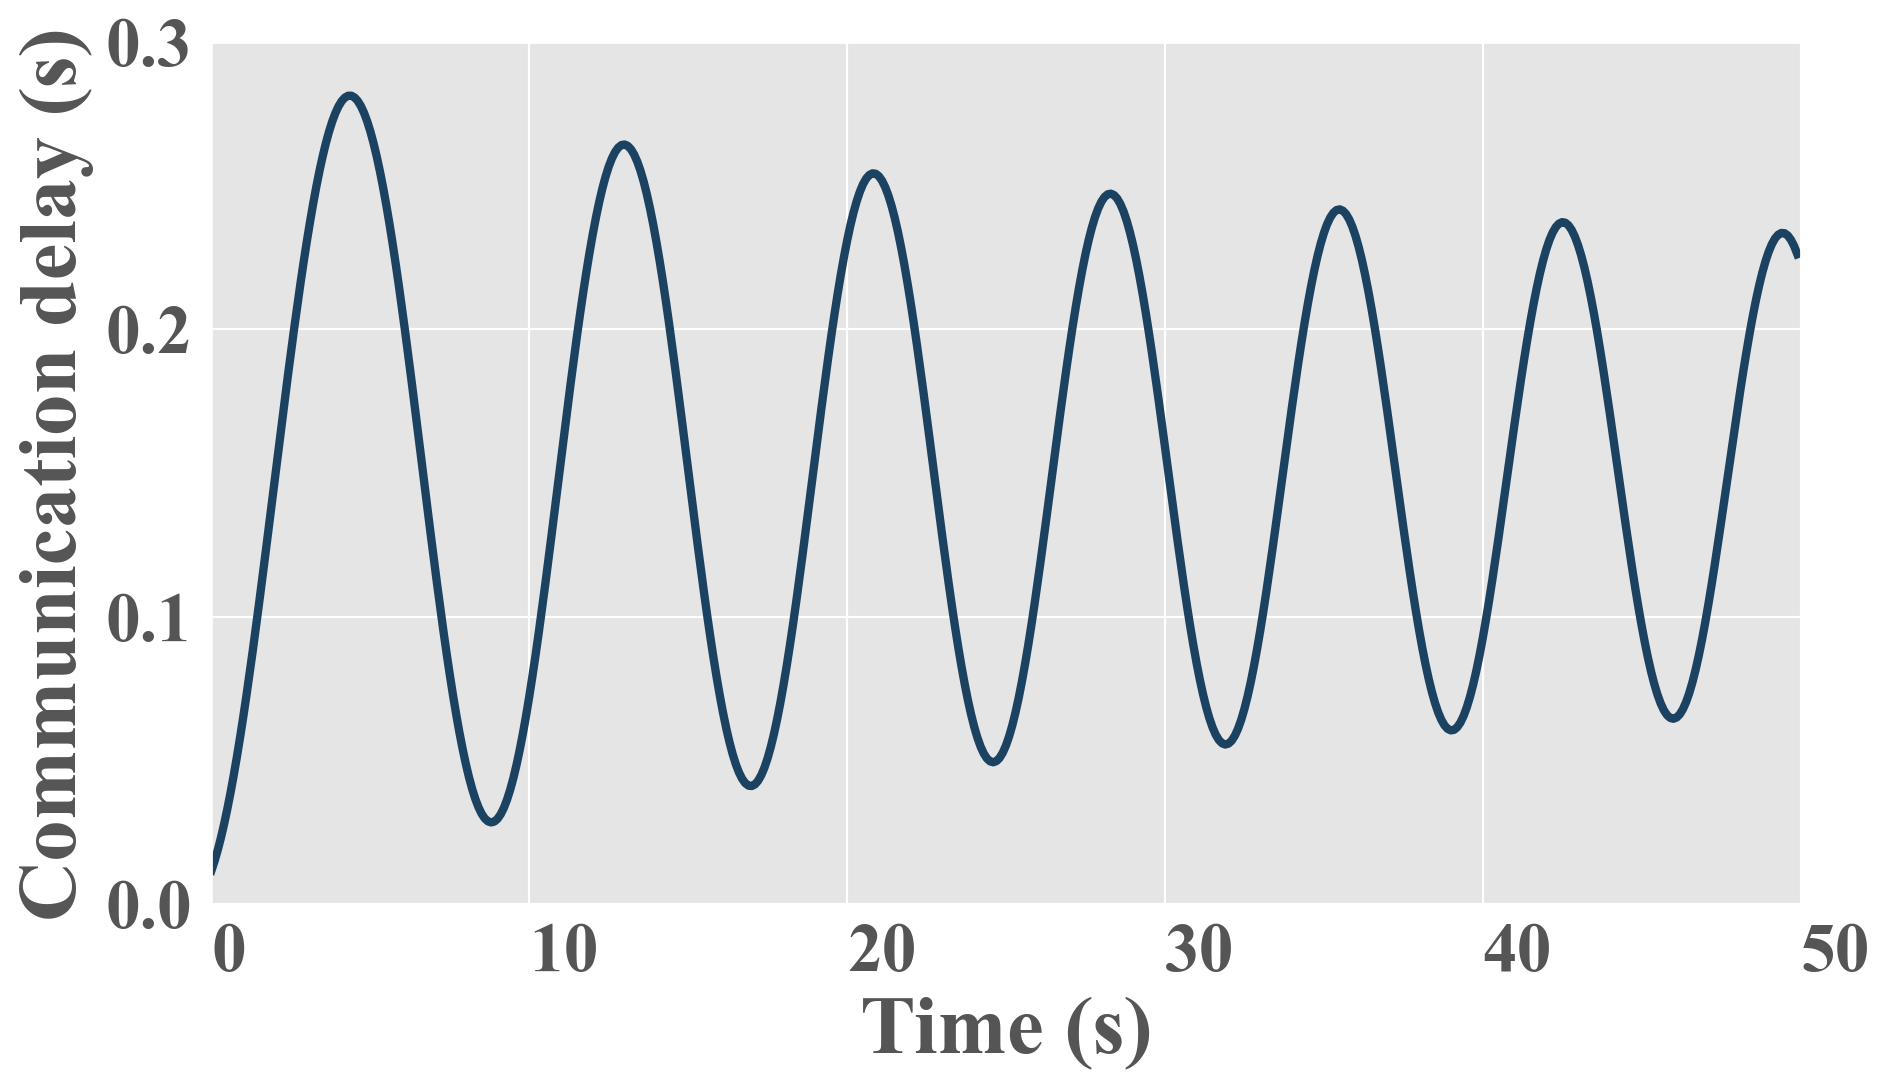
\includegraphics[width=7.5cm]{figs/fig2.png}
  \caption{~The curve of time-varying communication delay.}
  \label{fig2}
\end{figure}

\begin{table}
  \centering
  \setlength{\abovecaptionskip}{0pt}
  \setlength{\belowcaptionskip}{10pt}%设置标题与表格的距离
  \begin{threeparttable}[b]

    \caption{~Network and traffic simulation parameters.}
    \label{table1}
    {\begin{tabular}{lc} \toprule
        Parameters                                         & Value               \\ \midrule
        Platoon size $n$                                   & 5 vehicles          \\
        Vehicle length $L$                                 & 5 [m]               \\
        Engine actuator delay $\tau_i$                     & 0.2 [s] \tnote{1}   \\
        Weight of edge $\left( {i,j} \right) \quad a_{ij}$ & $\frac{1}{{{d_i}}}$ \\
        Minimum communication delay $h_{m}$                & 0 [m]               \\
        Maximum communication delay $h_{M}$                & 0.3 [m]             \\
        Minimum communication delay slope $d_{m}$          & -0.1                \\
        Maximum communication delay slope $d_{M}$          & 0.1                 \\
        \bottomrule
      \end{tabular}}
    \begin{tablenotes}
      \item[1] \citep{Wang2018a,Zhou2020}
    \end{tablenotes}
  \end{threeparttable}
\end{table}

Furthermore, to assess the tracking performance of the CAV platoon under the PLF with varying feedback control gains, two representative leader maneuvers are adopted:
\begin{enumerate}
\item \textbf{Trapezoidal signal}: The leader suddenly decelerates to $14.6m/s$ at a rate of $ - 0.15m/{s^2}$ and maintains this velocity for $36s$. Subsequently, the leader accelerates back to $20m/s$ at $ 0.3m/{s^2}$ (see Fig.\ref{fig3}(a, b)).
\item \textbf{Oscillation signal}: The leader abruptly accelerates to $23.6m/s$ within $12s$ and holds this velocity for $15s$. Then, the leader decelerates to $16.4m/s$ over $12s$ and accelerates back to $20m/s$ in $12s$ (see Fig.\ref{fig3}(c, d)).
\end{enumerate}


\begin{figure}

  \centering
  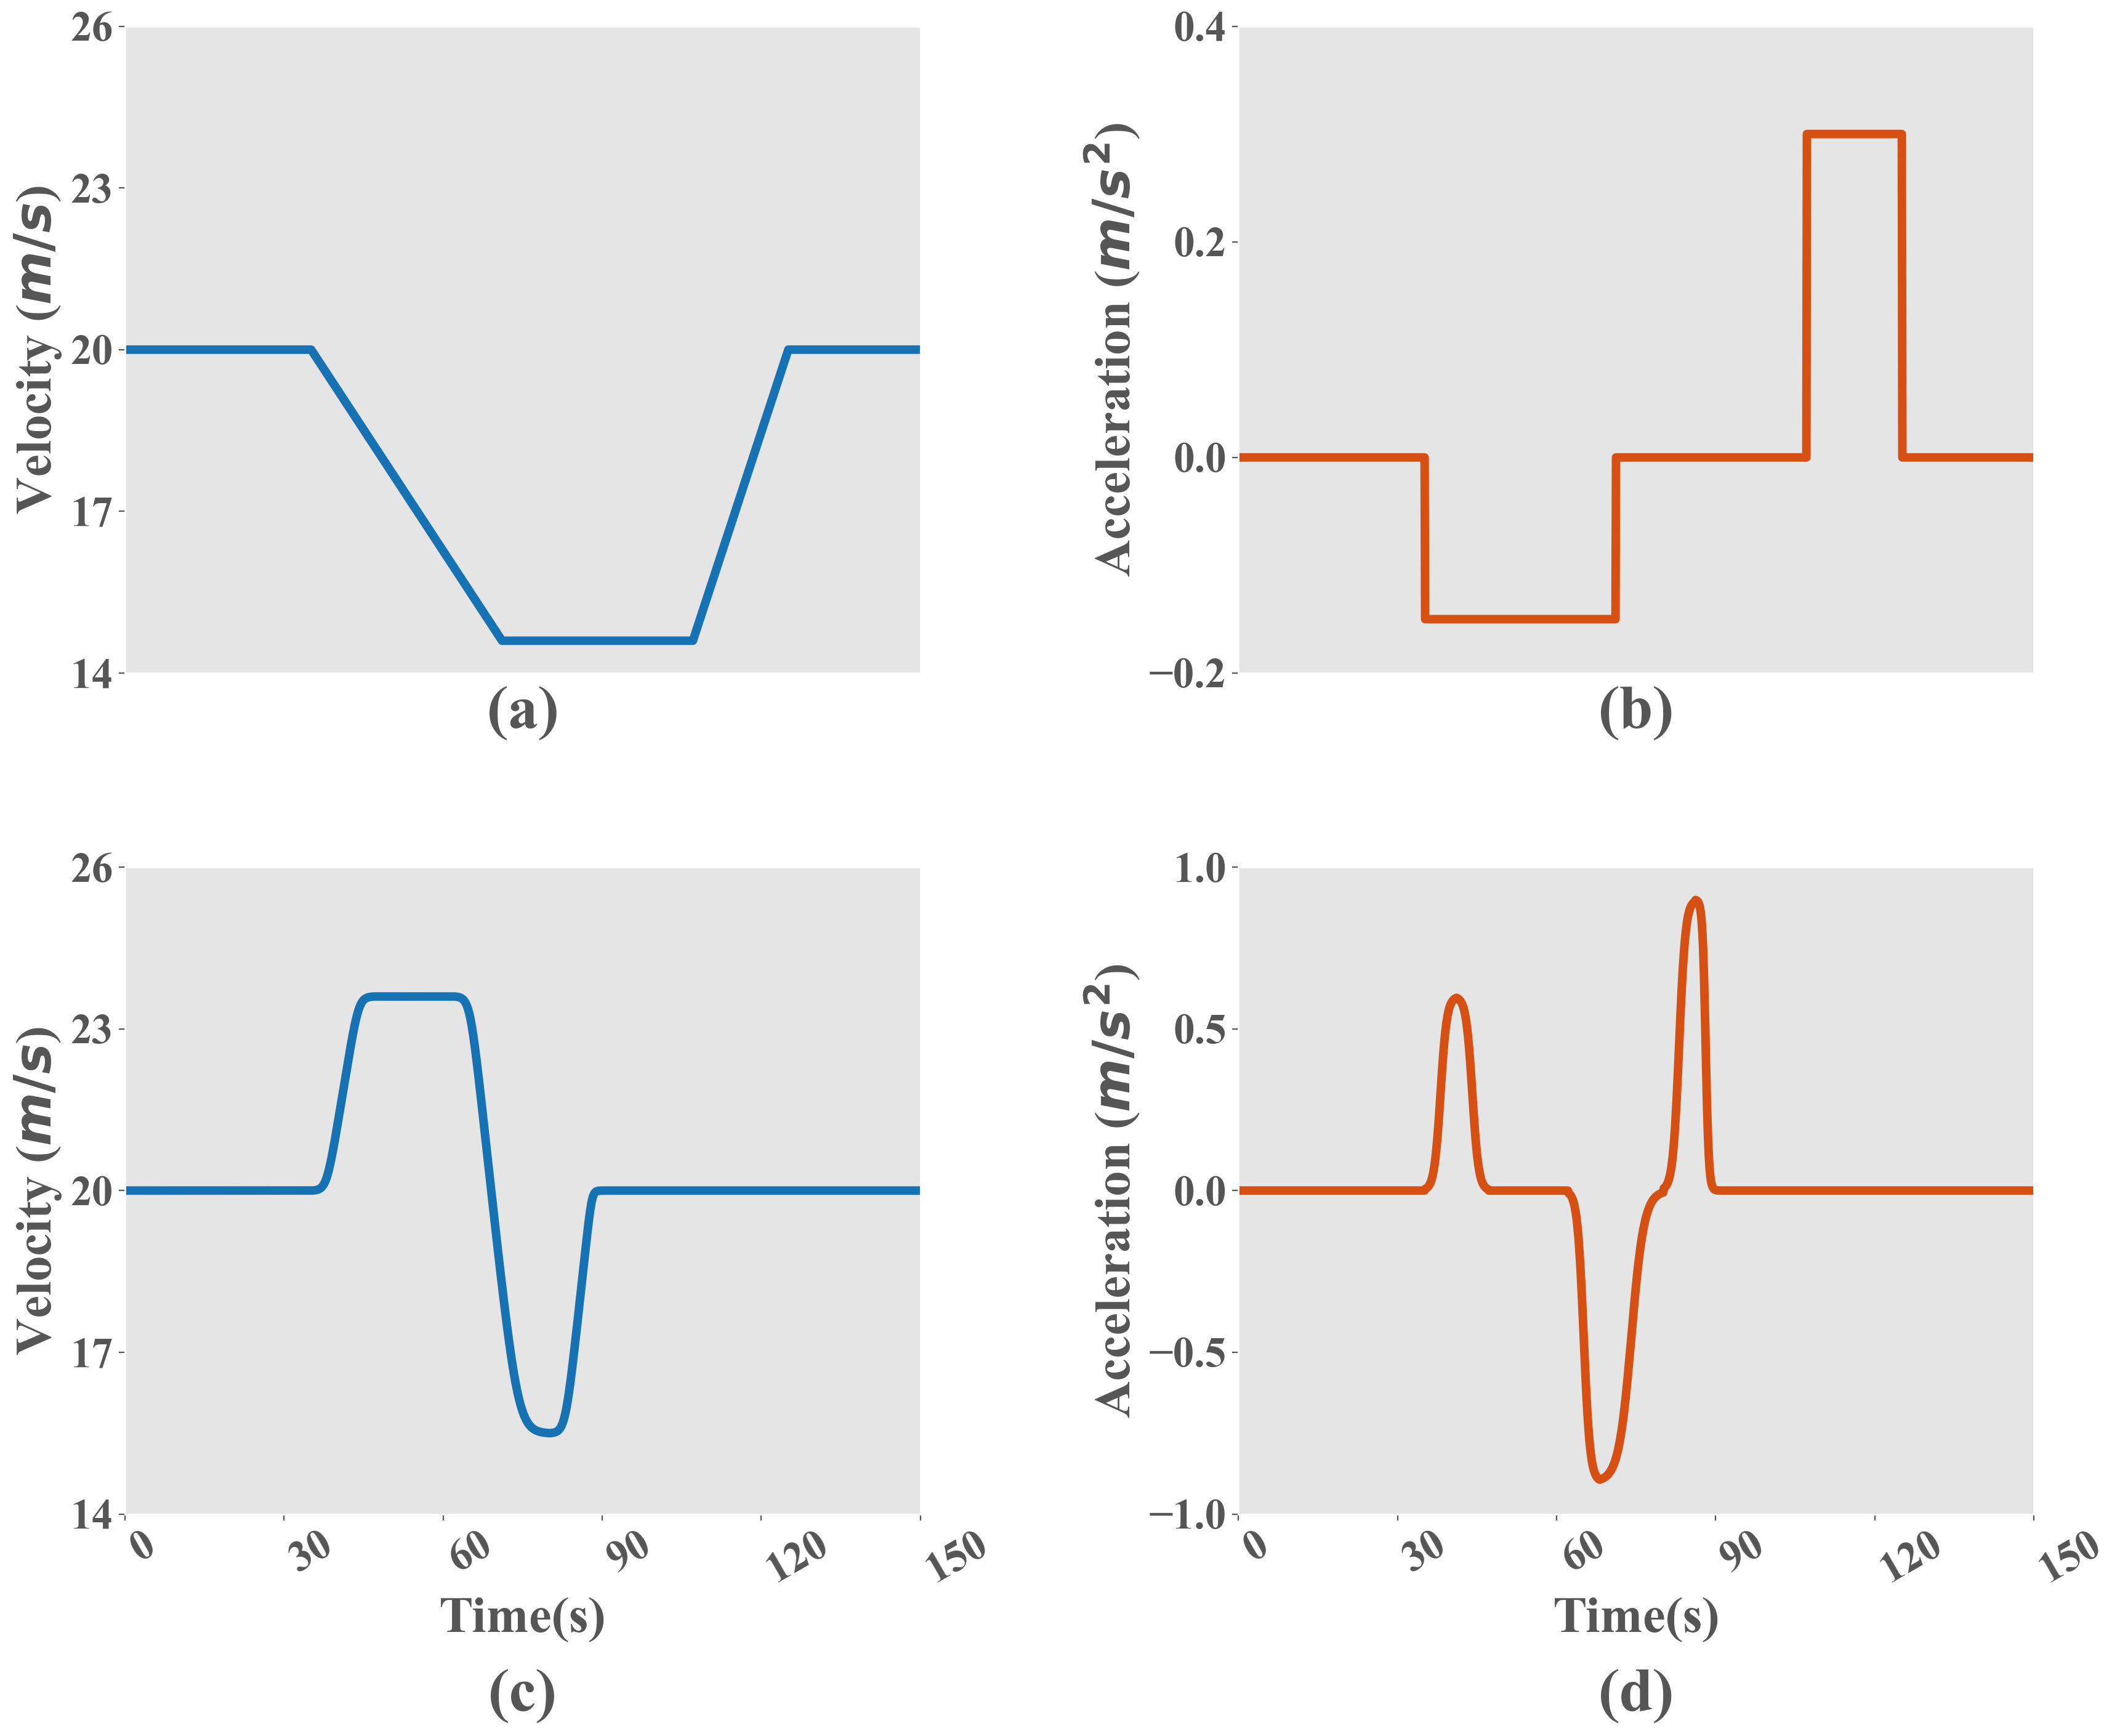
\includegraphics[width=8.5cm]{figs/fig3.png}
  \caption{~The two representative leader maneuvers: (a) and (b) denotes the velocity and acceleration of the trapezoidal signal, respectively; (c) and (d) denote the velocity and acceleration of the oscillation signal, respectively.}
  \label{fig3}

\end{figure}


\subsection{Numerical analyses of the CAV platoon under the PLF}
\label{Section 5.2}
In this subsection, the analysis concentrates on the CAV platoon that employs the PLF, using the same control parameters for each CAV in the platoon, in accordance with the conditions of Theorem~\ref{theorem6}. The influence of tracking performance with varying feedback control gains is explored by selecting four feedback control gains:
\begin{enumerate}
\item \textit{Parameter \uppercase\expandafter{\romannumeral1}:} $ {k_i} = {[0.3,0.3,0.3]^T} $;
\item \textit{Parameter \uppercase\expandafter{\romannumeral2}:} $ {k_i} = {[1,0.3,0.3]^T} $;
\item \textit{Parameter \uppercase\expandafter{\romannumeral3}:} $ {k_i} = {[0.3,1,0.3]^T} $;
\item \textit{Parameter \uppercase\expandafter{\romannumeral4}:} $ {k_i} = {[0.3,0.3,1]^T} $.
\end{enumerate}

Furthermore, the desired time headway is set to $ {h_i} = 0.6s $ \citep{li2017evaluation,ploeg2011connect}. The corresponding matrices $ P,S,Q,R, $ and $X$ are provided in Appendix C. A detailed analysis is conducted on the tracking performance and safety conditions.

\subsubsection{Tracking performance analyses}
\label{Section 5.2.1}


Upon the formation of the CAV platoon and reaching the equilibrium state where the tracking error is zero, the tracking performance of the four feedback control gains under investigation is assessed using the trapezoidal signal depicted in Fig.\ref{fig3}(a,b) as the leader maneuver. The results are presented in Fig.\ref{fig4}, which illustrates the tracking of the leader motion by the various CAVs in the platoon.

As anticipated from the theoretical outcomes, all CAVs can smoothly track the leader motion with a steady-state error of 0. Transient variations in the leader motion can provoke abrupt changes in the tracking error, which decrease over time due to stability. Moreover, the impact of different feedback control gains on the tracking performance varies, as demonstrated by comparing the results of the four control gains. Elevating the gain of the spacing and velocity errors significantly diminishes the overshoot of the acceleration curve, particularly in the case of the velocity error gain, where the overshoot is effectively suppressed. However, augmenting the gain of the spacing error results in oscillations in the acceleration curve, potentially owing to time-varying delay. Conversely, increasing the gain of the acceleration error adversely affects the tracking performance because of dramatic fluctuations, even though stability is maintained. Consequently, regarding control parameter selection, enhancing the gain of the velocity error within an appropriate range can improve the tracking performance to some extent.



\begin{figure*}

  \centering
  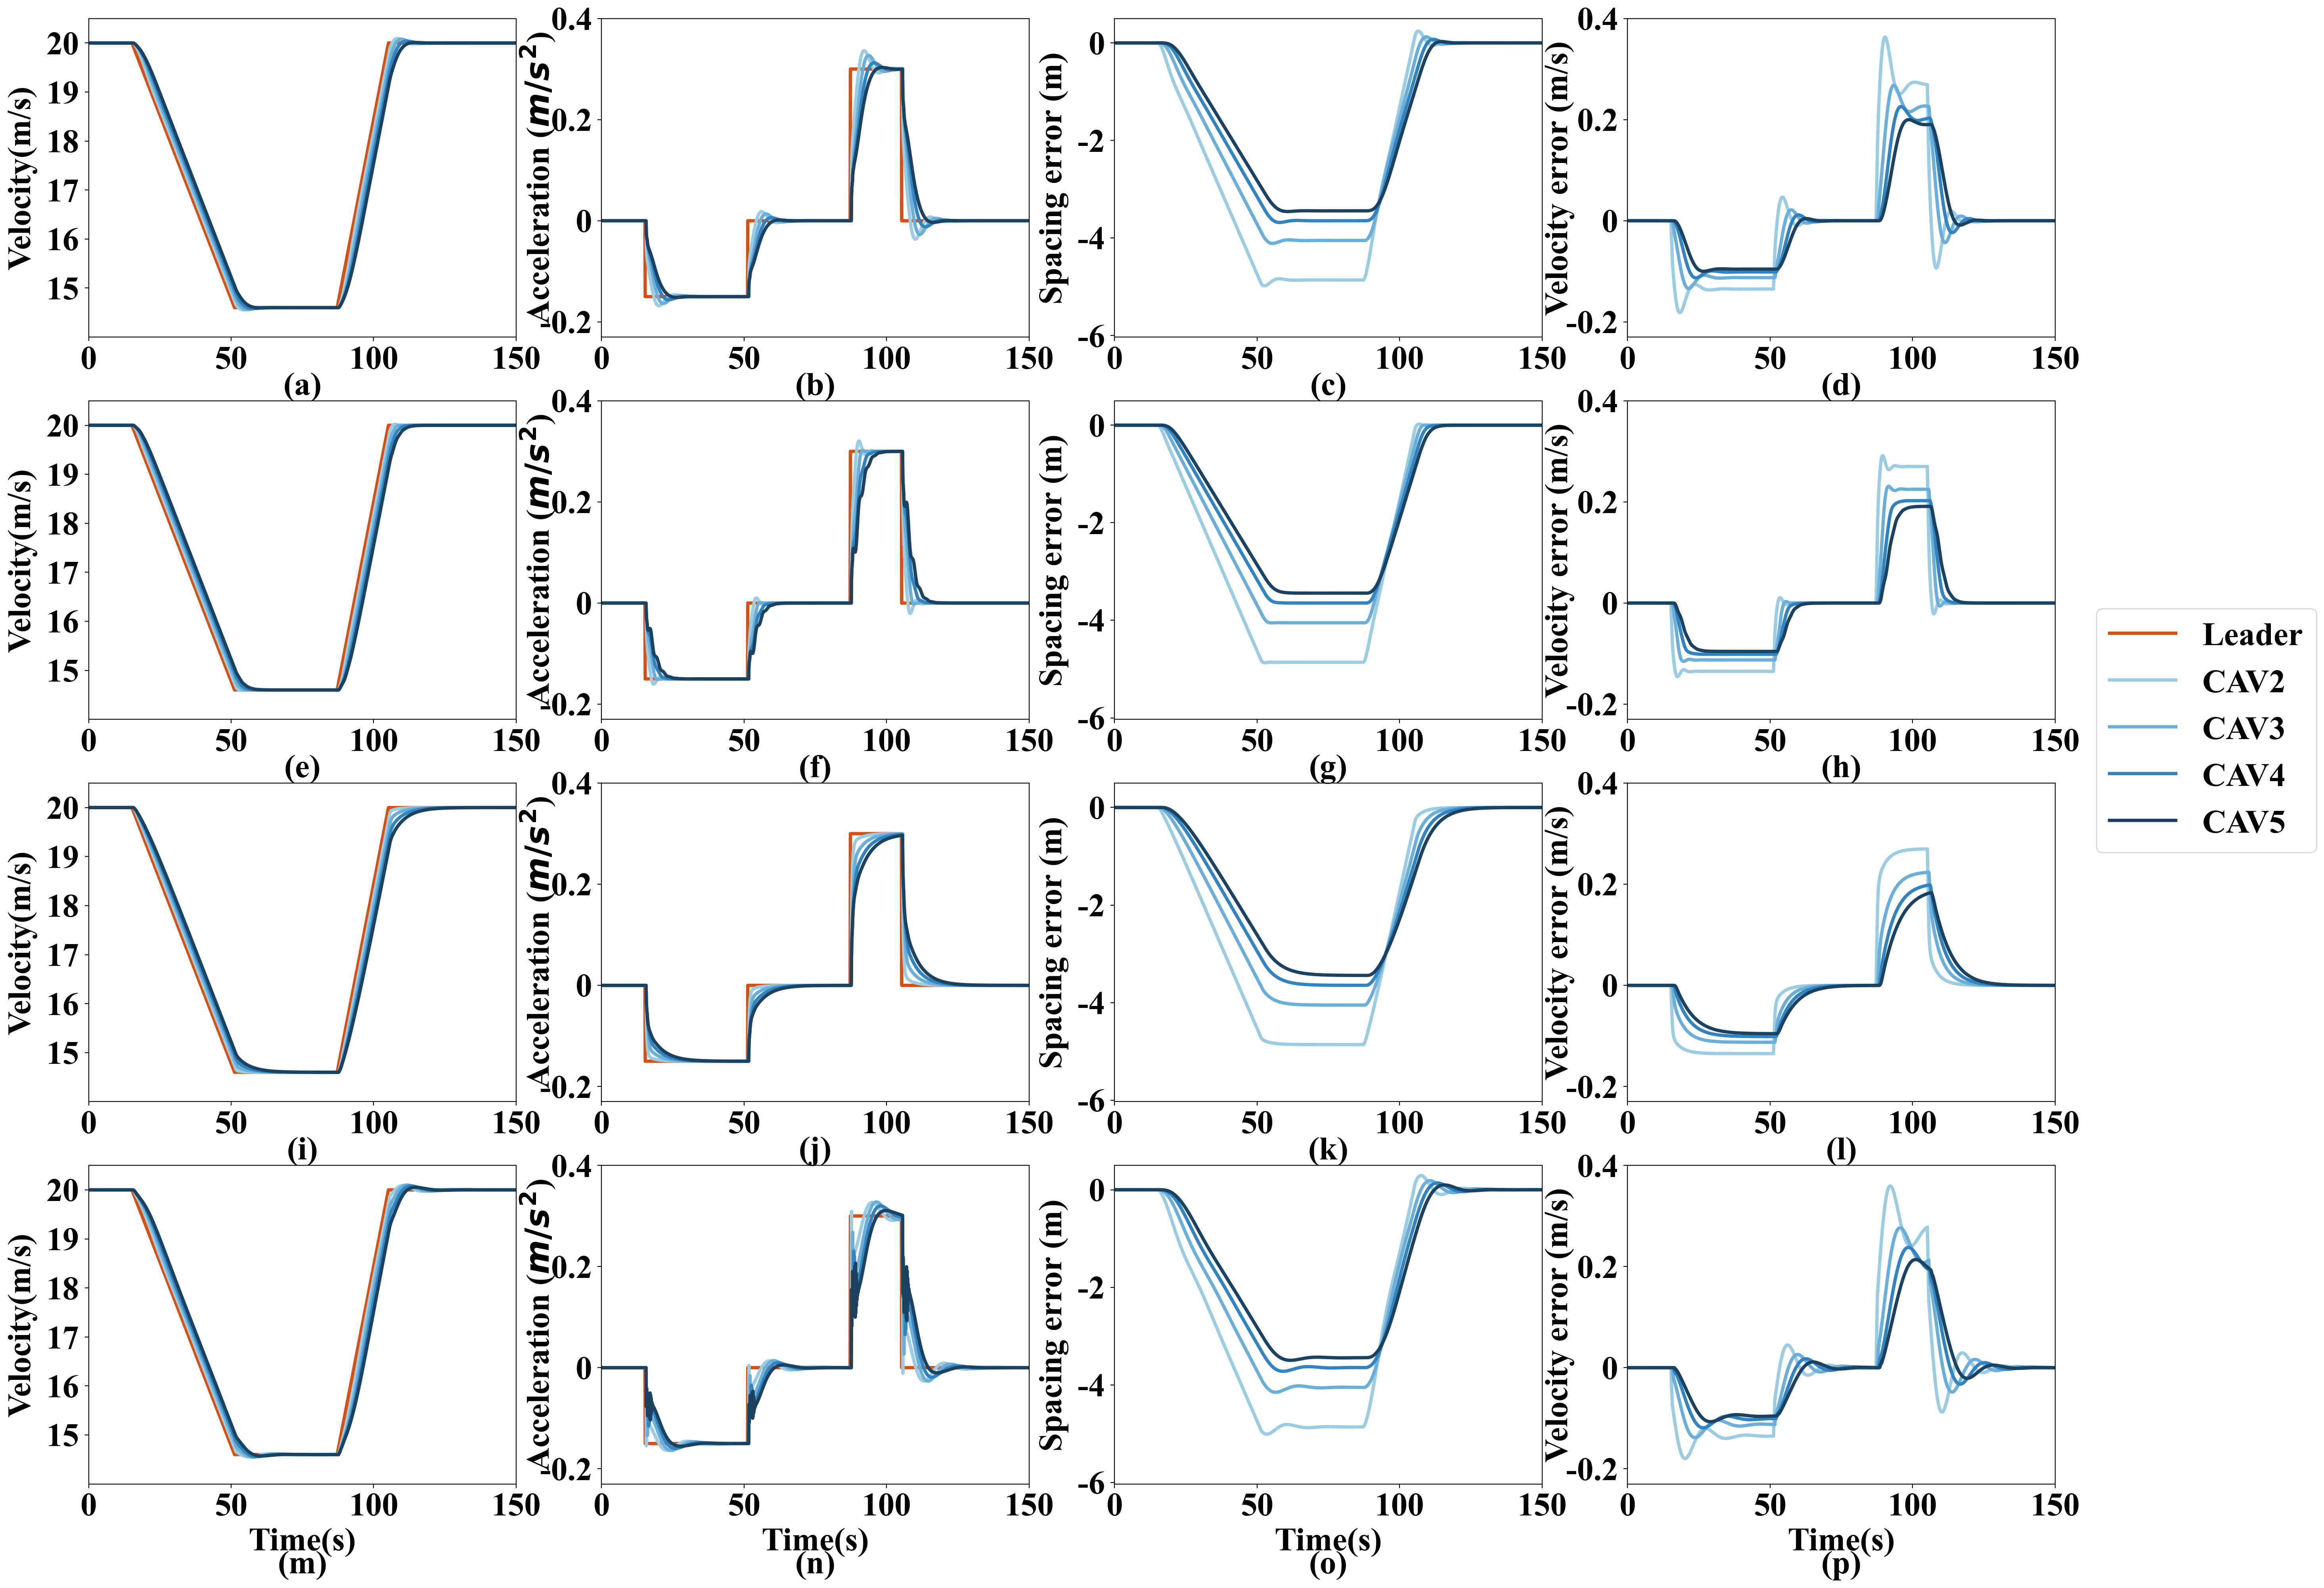
\includegraphics[width=16cm]{figs/fig4.png}
  \caption{~The tracking performance of the CAV platoon for the Trapezoidal signal in Fig. 3(a,b) under the four feedback control gains is as follows: (a), (b), (c), and (d) display the tracking results under Parameter \uppercase\expandafter{\romannumeral1}, including the velocity, acceleration, tracking error of spacing, and tracking error of velocity, respectively; (e), (f), (g), and (h) depict the case under Parameter \uppercase\expandafter{\romannumeral2}; (i), (j), (k), and (l) represent the case under Parameter \uppercase\expandafter{\romannumeral3}; (m), (n), (o), and (p) illustrate the case under Parameter \uppercase\expandafter{\romannumeral4}.}
  \label{fig4}
\end{figure*}

\begin{figure*}

  \centering
  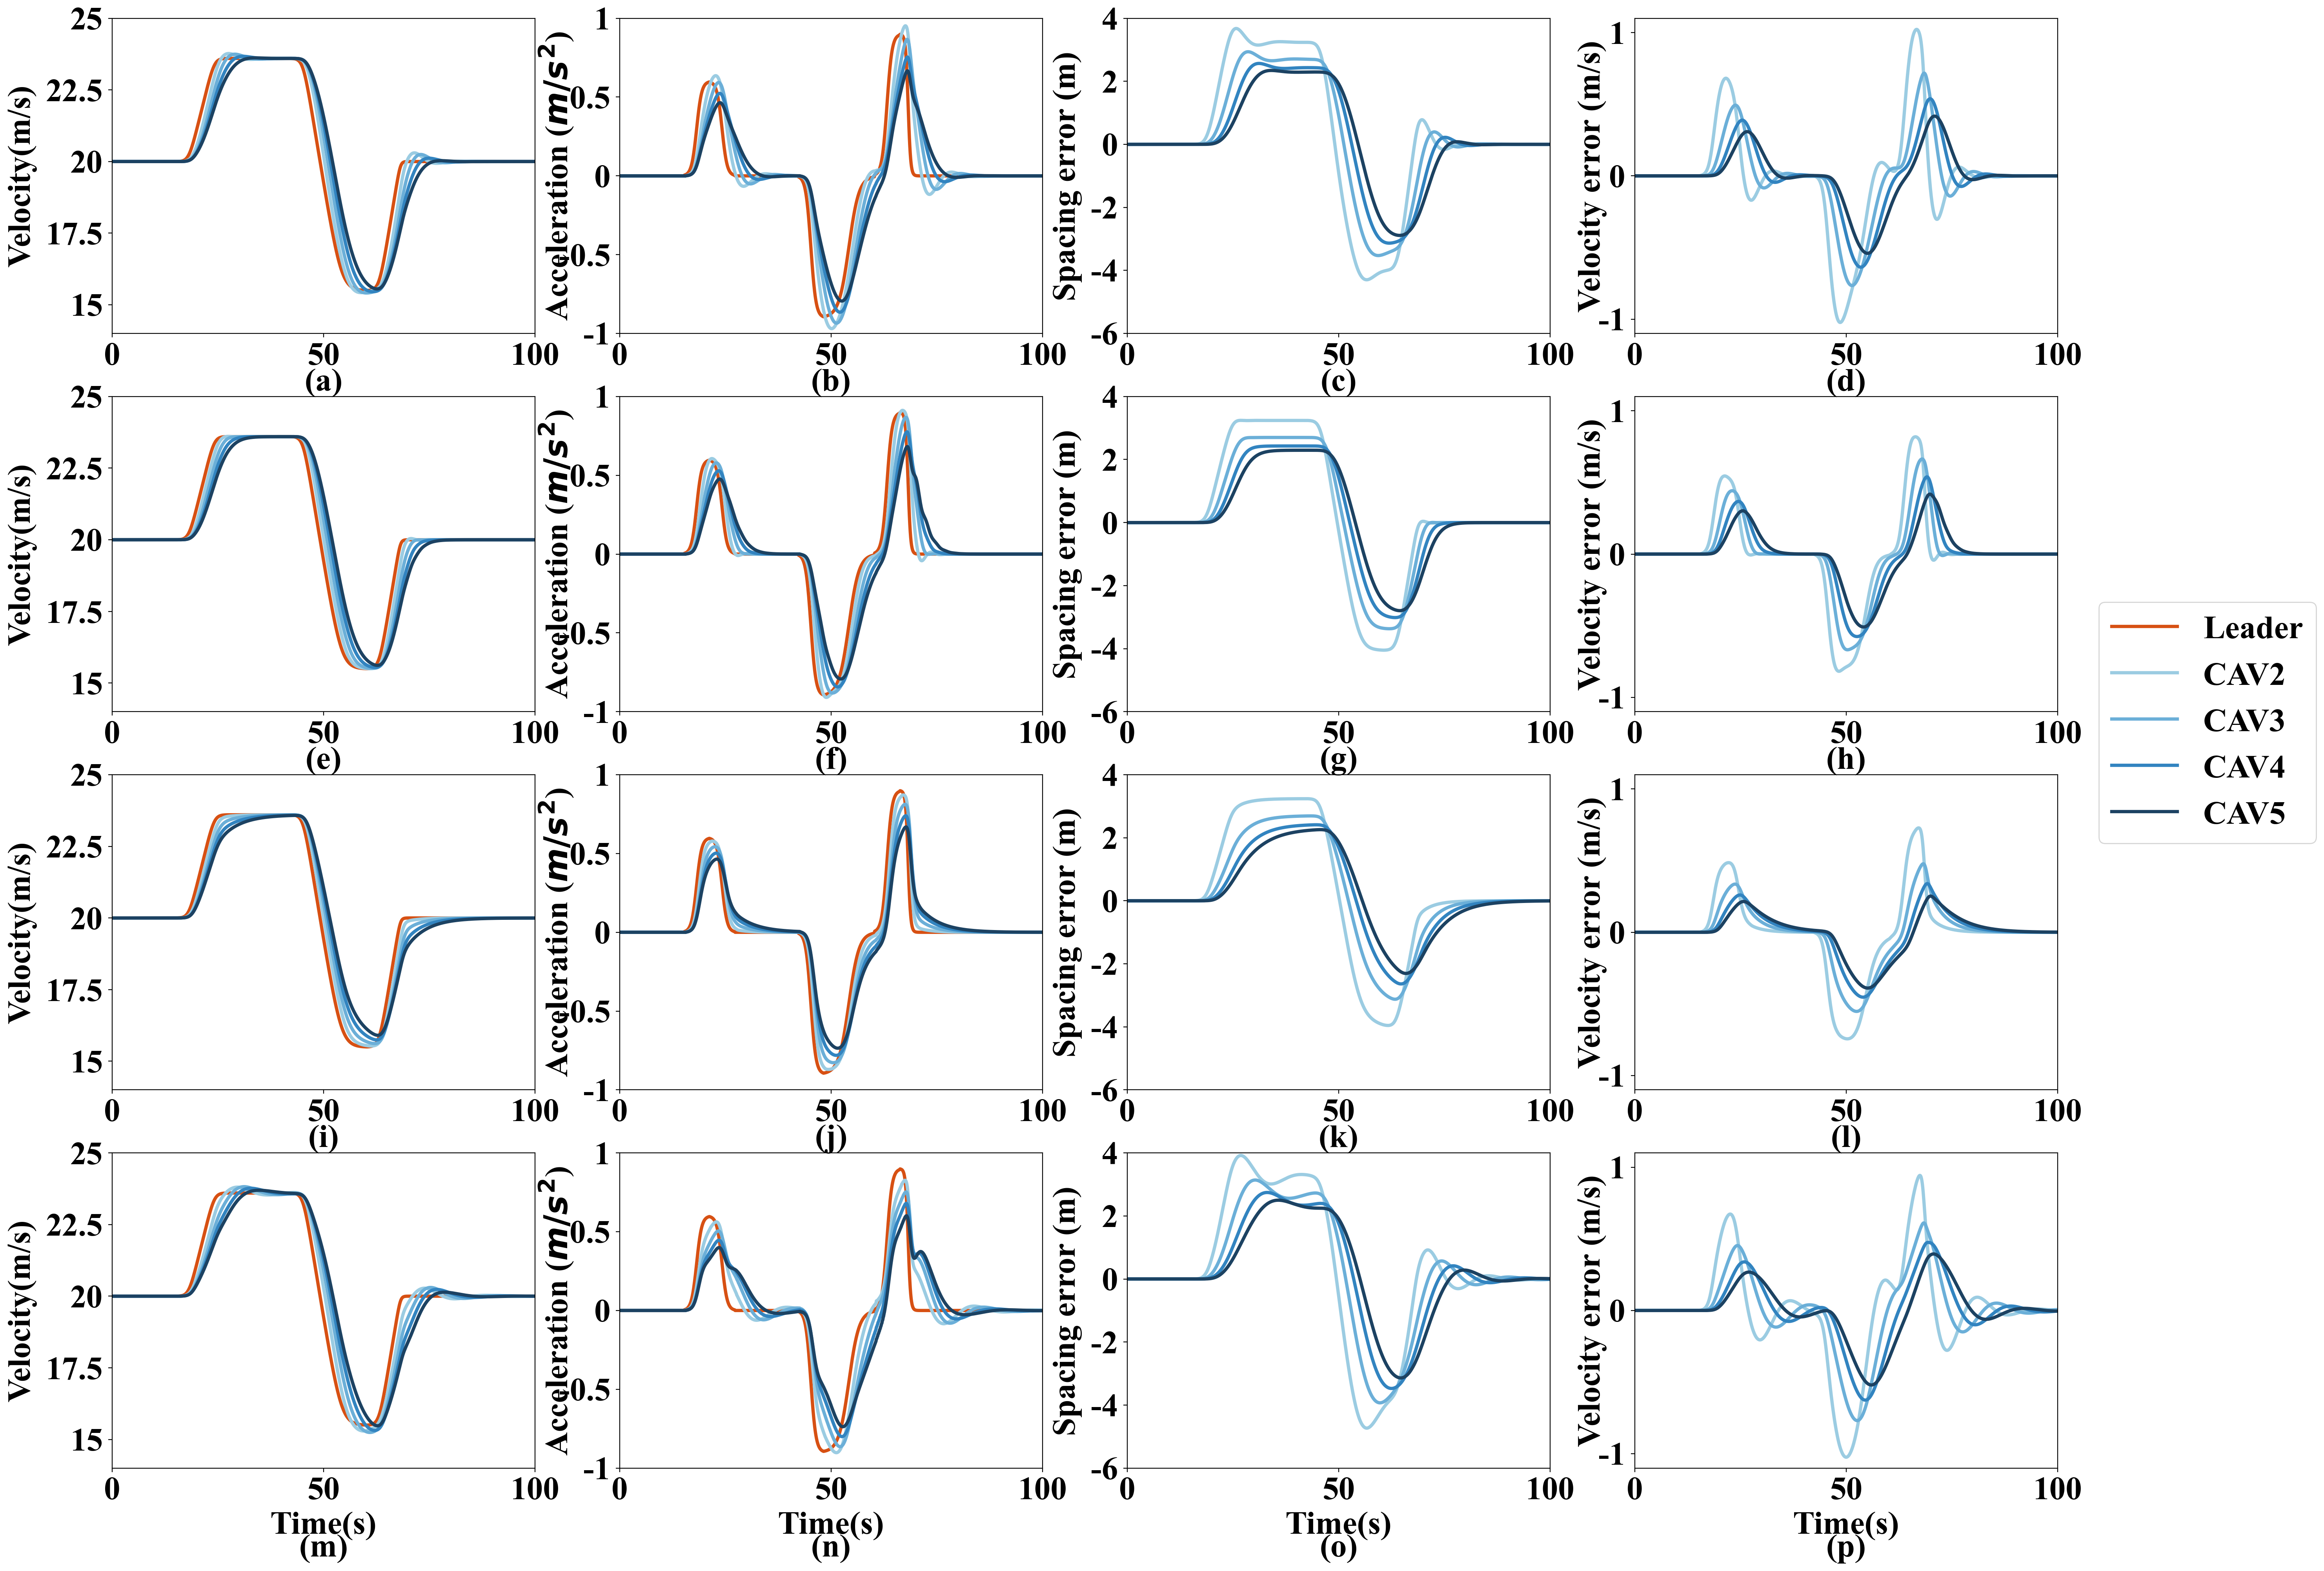
\includegraphics[width=16cm]{figs/fig5.png}
  \caption{~The tracking performance of the CAV platoon for the Oscillation signal in Fig. 3(c,d) under the four feedback control gains is as follows: (a), (b), (c), and (d) display the tracking results under Parameter \uppercase\expandafter{\romannumeral1}, including the velocity, acceleration, tracking error of spacing, and tracking error of velocity, respectively; (e), (f), (g), and (h) depict the case under Parameter \uppercase\expandafter{\romannumeral2}; (i), (j), (k), and (l) represent the case under Parameter \uppercase\expandafter{\romannumeral3}; (m), (n), (o), and (p) illustrate the case under Parameter \uppercase\expandafter{\romannumeral4}.}
  \label{fig5}
\end{figure*}

Moreover, the tracking performance of the four feedback control gains is assessed under the oscillation signal presented in Fig.\ref{fig3}(c, d). Fig.\ref{fig5} displays the corresponding tracking performance for the four feedback control gains. Under the oscillation signal, all cases with the four feedback control gains maintain excellent tracking performance, with each vehicle adjusting to changes in leader motion and returning to the equilibrium state with zero steady-state error. A similar phenomenon and conclusion as in Fig.\ref{fig4} can be observed, indicating that increasing the gain of spacing and velocity errors can benefit tracking performance, while increasing the gain of acceleration errors does not necessarily provide the same benefits.

Additionally, to complement the analysis on stability through tracking performance, two widely accepted indicators, namely Setting Time (ST) and Number of Oscillations (NOO), are employed for evaluating the transient response performance of different feedback control gains \citep{bennett1993history,sontag2013mathematical}. ST is defined as "the time required for the response curve to reach and stay within a range of a certain percentage (2\%) of the final value," while NOO is "the number of deviations of the response curve from the final value caused by errors in the setting time." Both ST and NOO are crucial measures of transient response, with ST representing the speed of achieving equilibrium and NOO representing the accuracy and comfort of the response. Since the investigation focuses on the differences in the transient response of various feedback control gains, the form of leader motion has little impact, and thus the results are analyzed here only for the Trapezoidal signal case.

\begin{figure*}

  \centering
  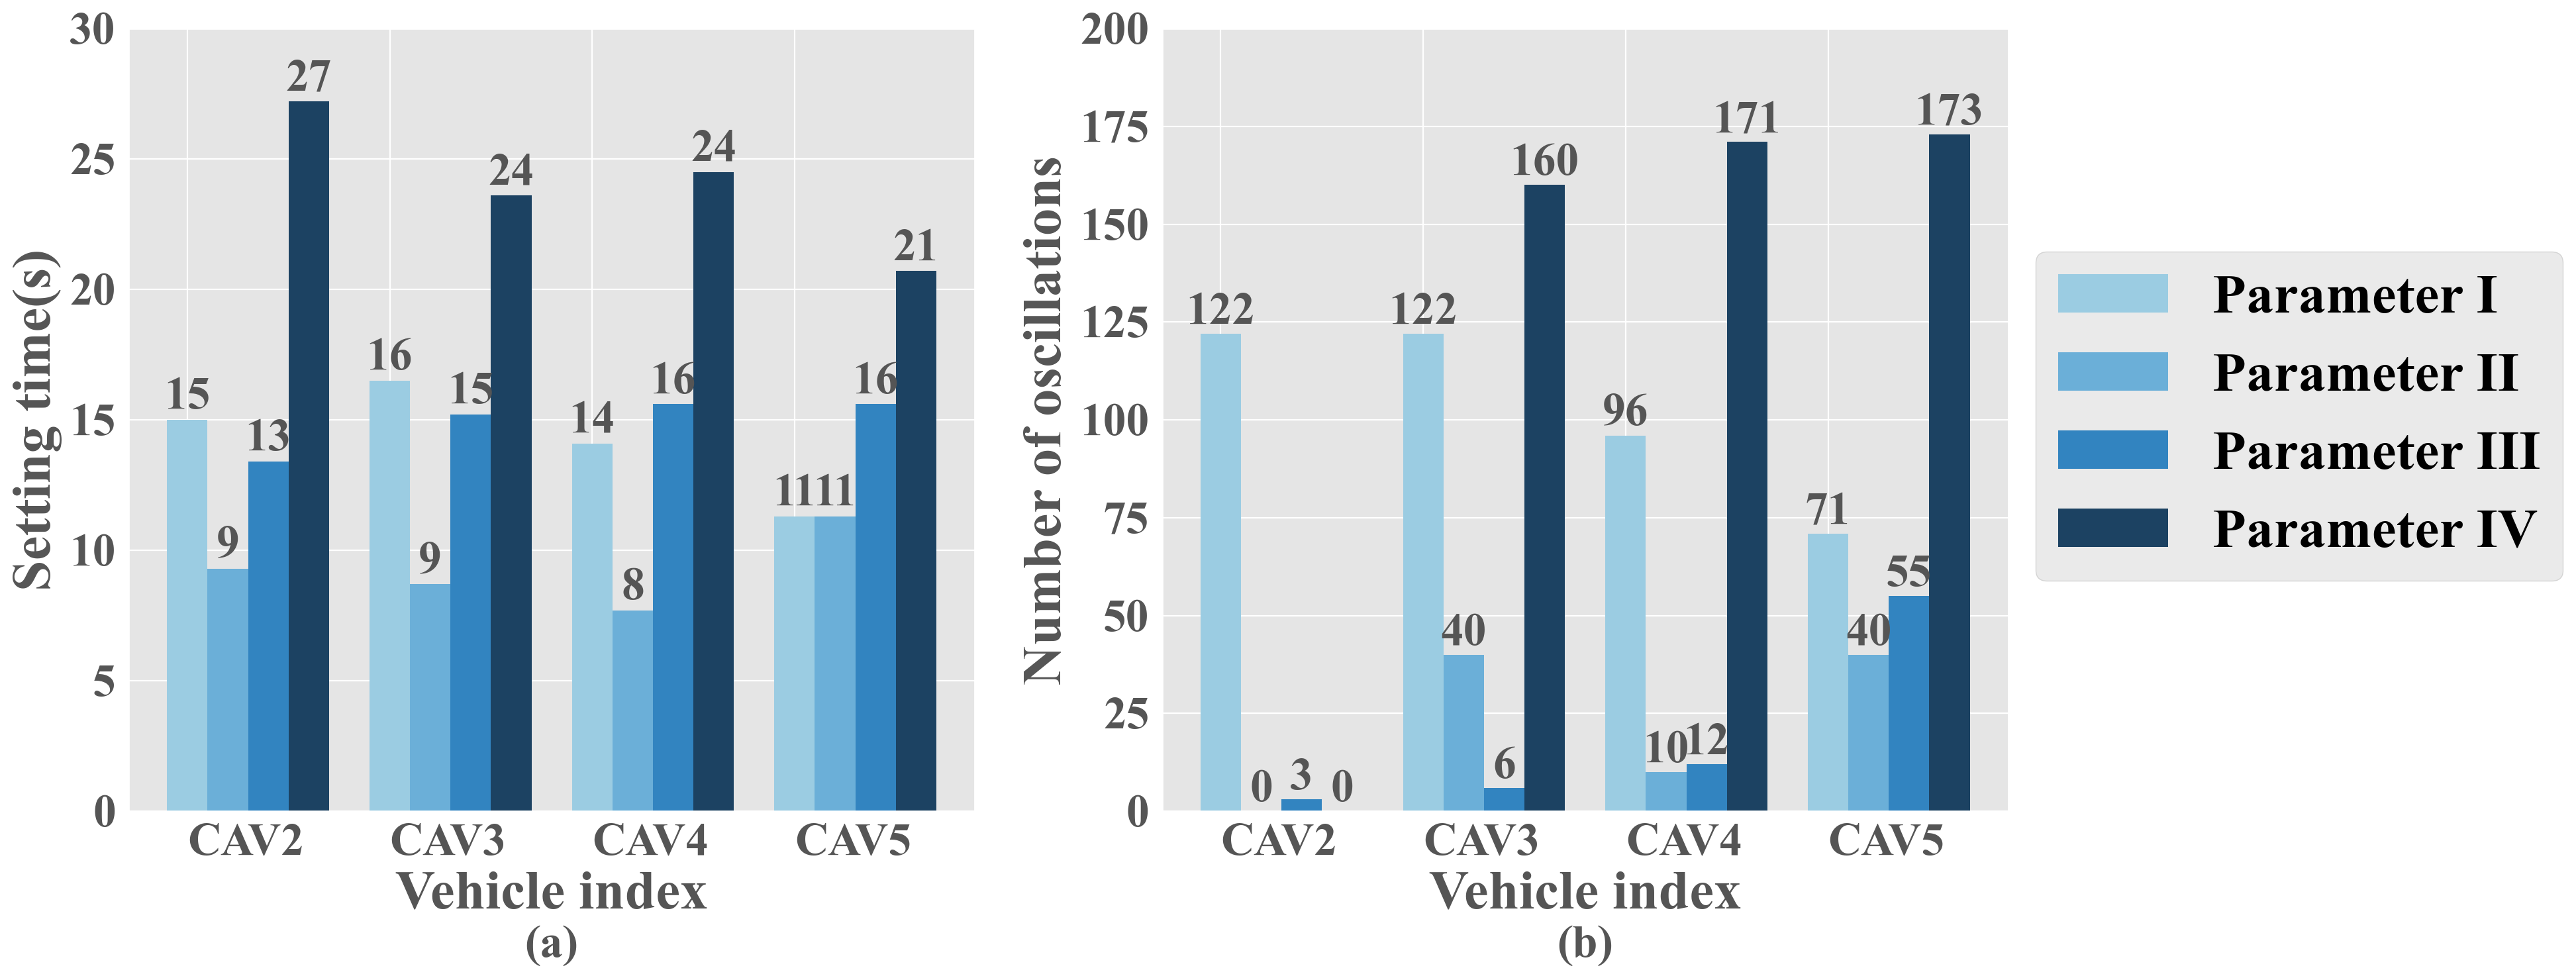
\includegraphics[width=16cm]{figs/fig6.png}
  \caption{~Indicators for evaluating the transient response of each CAV within the CAV platoon under the four feedback control gains: (a) the case of setting time; (b) the case of the number of oscillations.}
  \label{fig6}
\end{figure*}

Fig.\ref{fig6} compares the effects of different feedback control gains on two transient response indicators: Setting time (ST) and Number of oscillations (NOO). The results indicate that different control gains have a significant impact on transient response. Specifically, Parameter \uppercase\expandafter{\romannumeral2} and Parameter \uppercase\expandafter{\romannumeral3} show smaller ST and NOO than Parameter \uppercase\expandafter{\romannumeral1}, indicating that increasing the gain of spacing and velocity errors is effective in reducing velocity fluctuations and time from perturbation to equilibrium, thereby improving driving comfort and safety. However, increasing the gain of acceleration error, as in Parameter \uppercase\expandafter{\romannumeral4}, does not improve transient response. Moreover, for all control gain cases, the ST increases and NOO decreases with increasing vehicle index, suggesting that larger CAV platoons have less velocity fluctuation from perturbation to equilibrium, albeit with longer recovery times. Notably, Parameter \uppercase\expandafter{\romannumeral3} results in NOO=0, indicating no overshoot during transient response, and thus, performs well in terms of safety and comfort.


\subsubsection{Safety analyses considering hard braking maneuver}
\label{Section 5.2.2}

To further assess safety across various driving scenarios and feedback control gains, we conduct a quantitative analysis to examine the potential emergence of critical driving situations for all feedback control gains under investigation. This analysis utilizes the well-established safety indicator, Deceleration Rate to Avoid the Crash (DRAC), which has been extensively studied in the literature \citep{fu2021comparison,fu2021random}. This indicator presents the deceleration rate needed to be applied by a vehicle to avoid a collision with another vehicle which can be defined for each vehicle $i$ at the time $t$ as follows:
\begin{equation}
  DRA{C_i}(t) = \frac{{{{\left( {{v_i}(t) - {v_{i - 1}}(t)} \right)}^2}}}{{2\left( {{p_{i - 1}}(t) - {p_i}(t) - L} \right)}}.
  \label{eq522}
\end{equation}


Furthermore, an additional scenario was considered to evaluate safety across various driving scenarios and feedback control gains, specifically a hard braking maneuver where the Leader decelerates from $20m/s$ to $0m/s$ within $20s$. The reaction of the CAV platoon to this scenario for the four feedback control gains under investigation is displayed in Fig.\ref{fig7}. Notably, the CAVs in the platoon accurately track the Leader motion and decelerate to $0m/s$ without collision under each control gain. The DRAC of different CAVs under different control gains in the hard braking maneuver is presented as boxplots in Fig.\ref{fig8}, with the Leader's DRAC omitted due to its lack of a predecessor. The second through fifth CAVs in the platoon are denoted as CAV2, CAV3, CAV4, and CAV5, respectively.



\begin{figure}

  \centering
  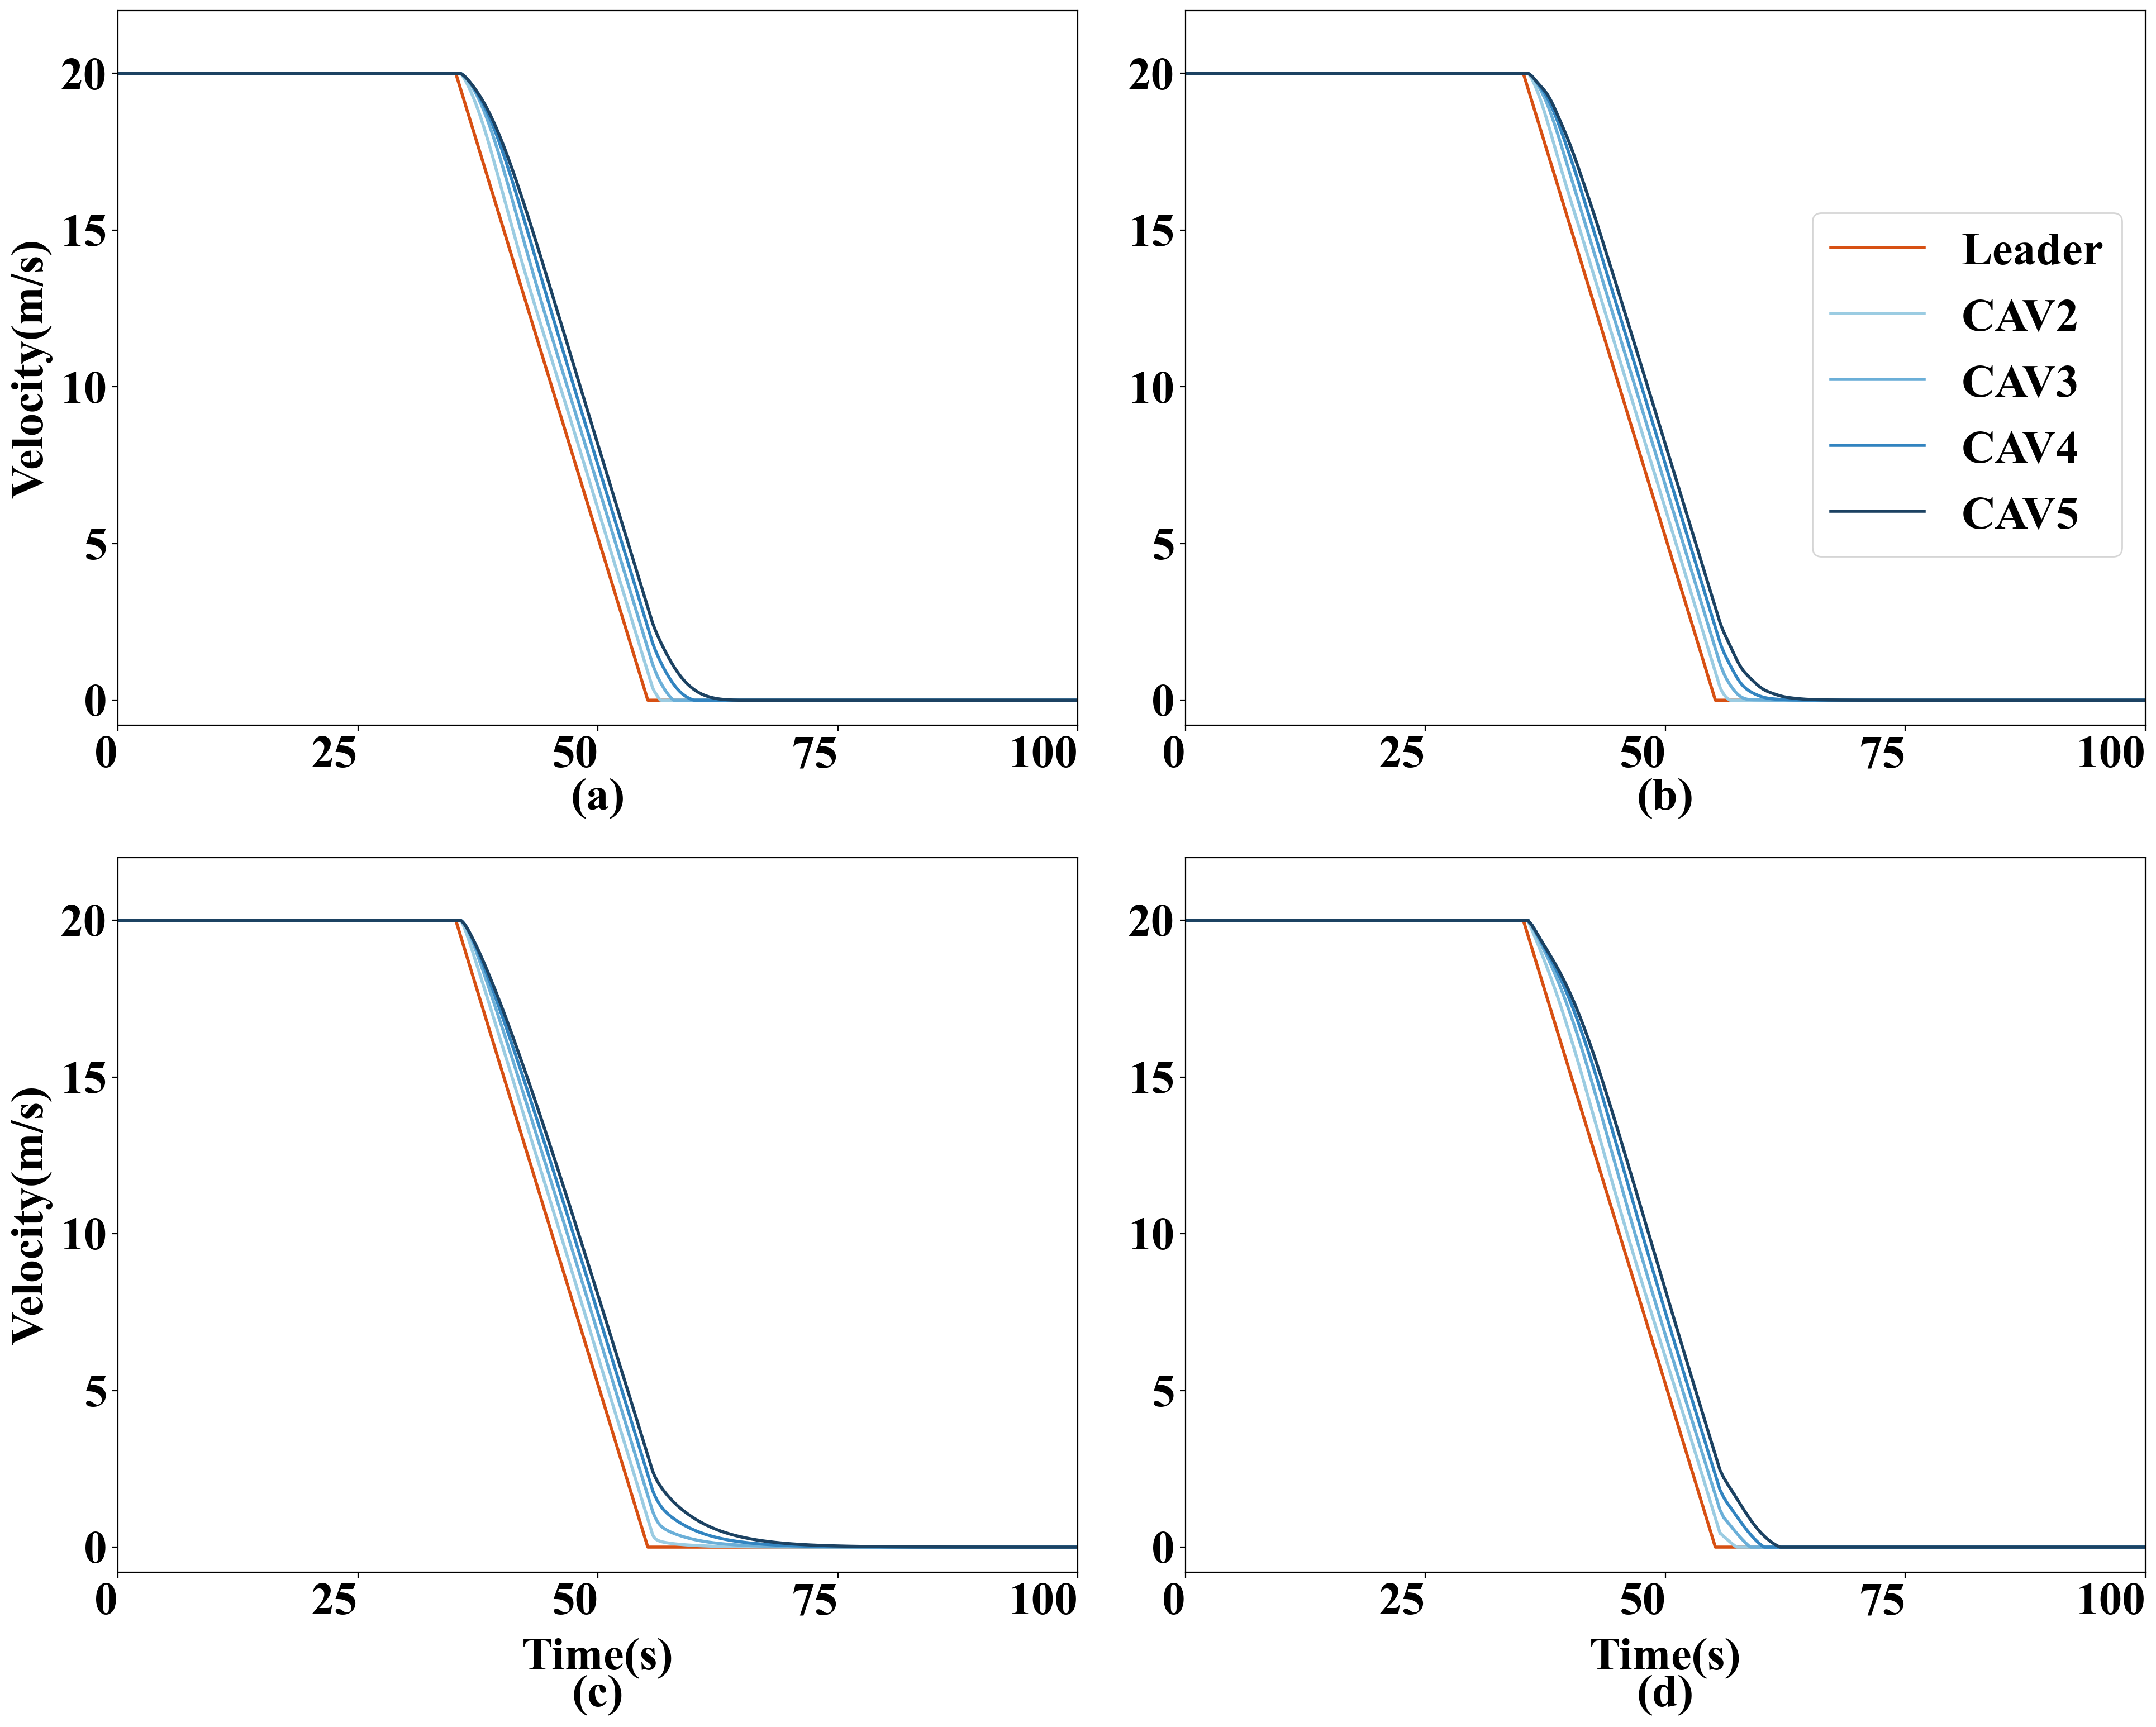
\includegraphics[width=8.5cm]{figs/fig7.png}
  \caption{~The tracking performance for a hard braking maneuver for each feedback control gain under investigation: (a) Parameter \uppercase\expandafter{\romannumeral1}; (b) Parameter \uppercase\expandafter{\romannumeral2}; (c) Parameter \uppercase\expandafter{\romannumeral3}; (d) Parameter \uppercase\expandafter{\romannumeral4}.}
  \label{fig7}
\end{figure}


\begin{figure}

  \centering
  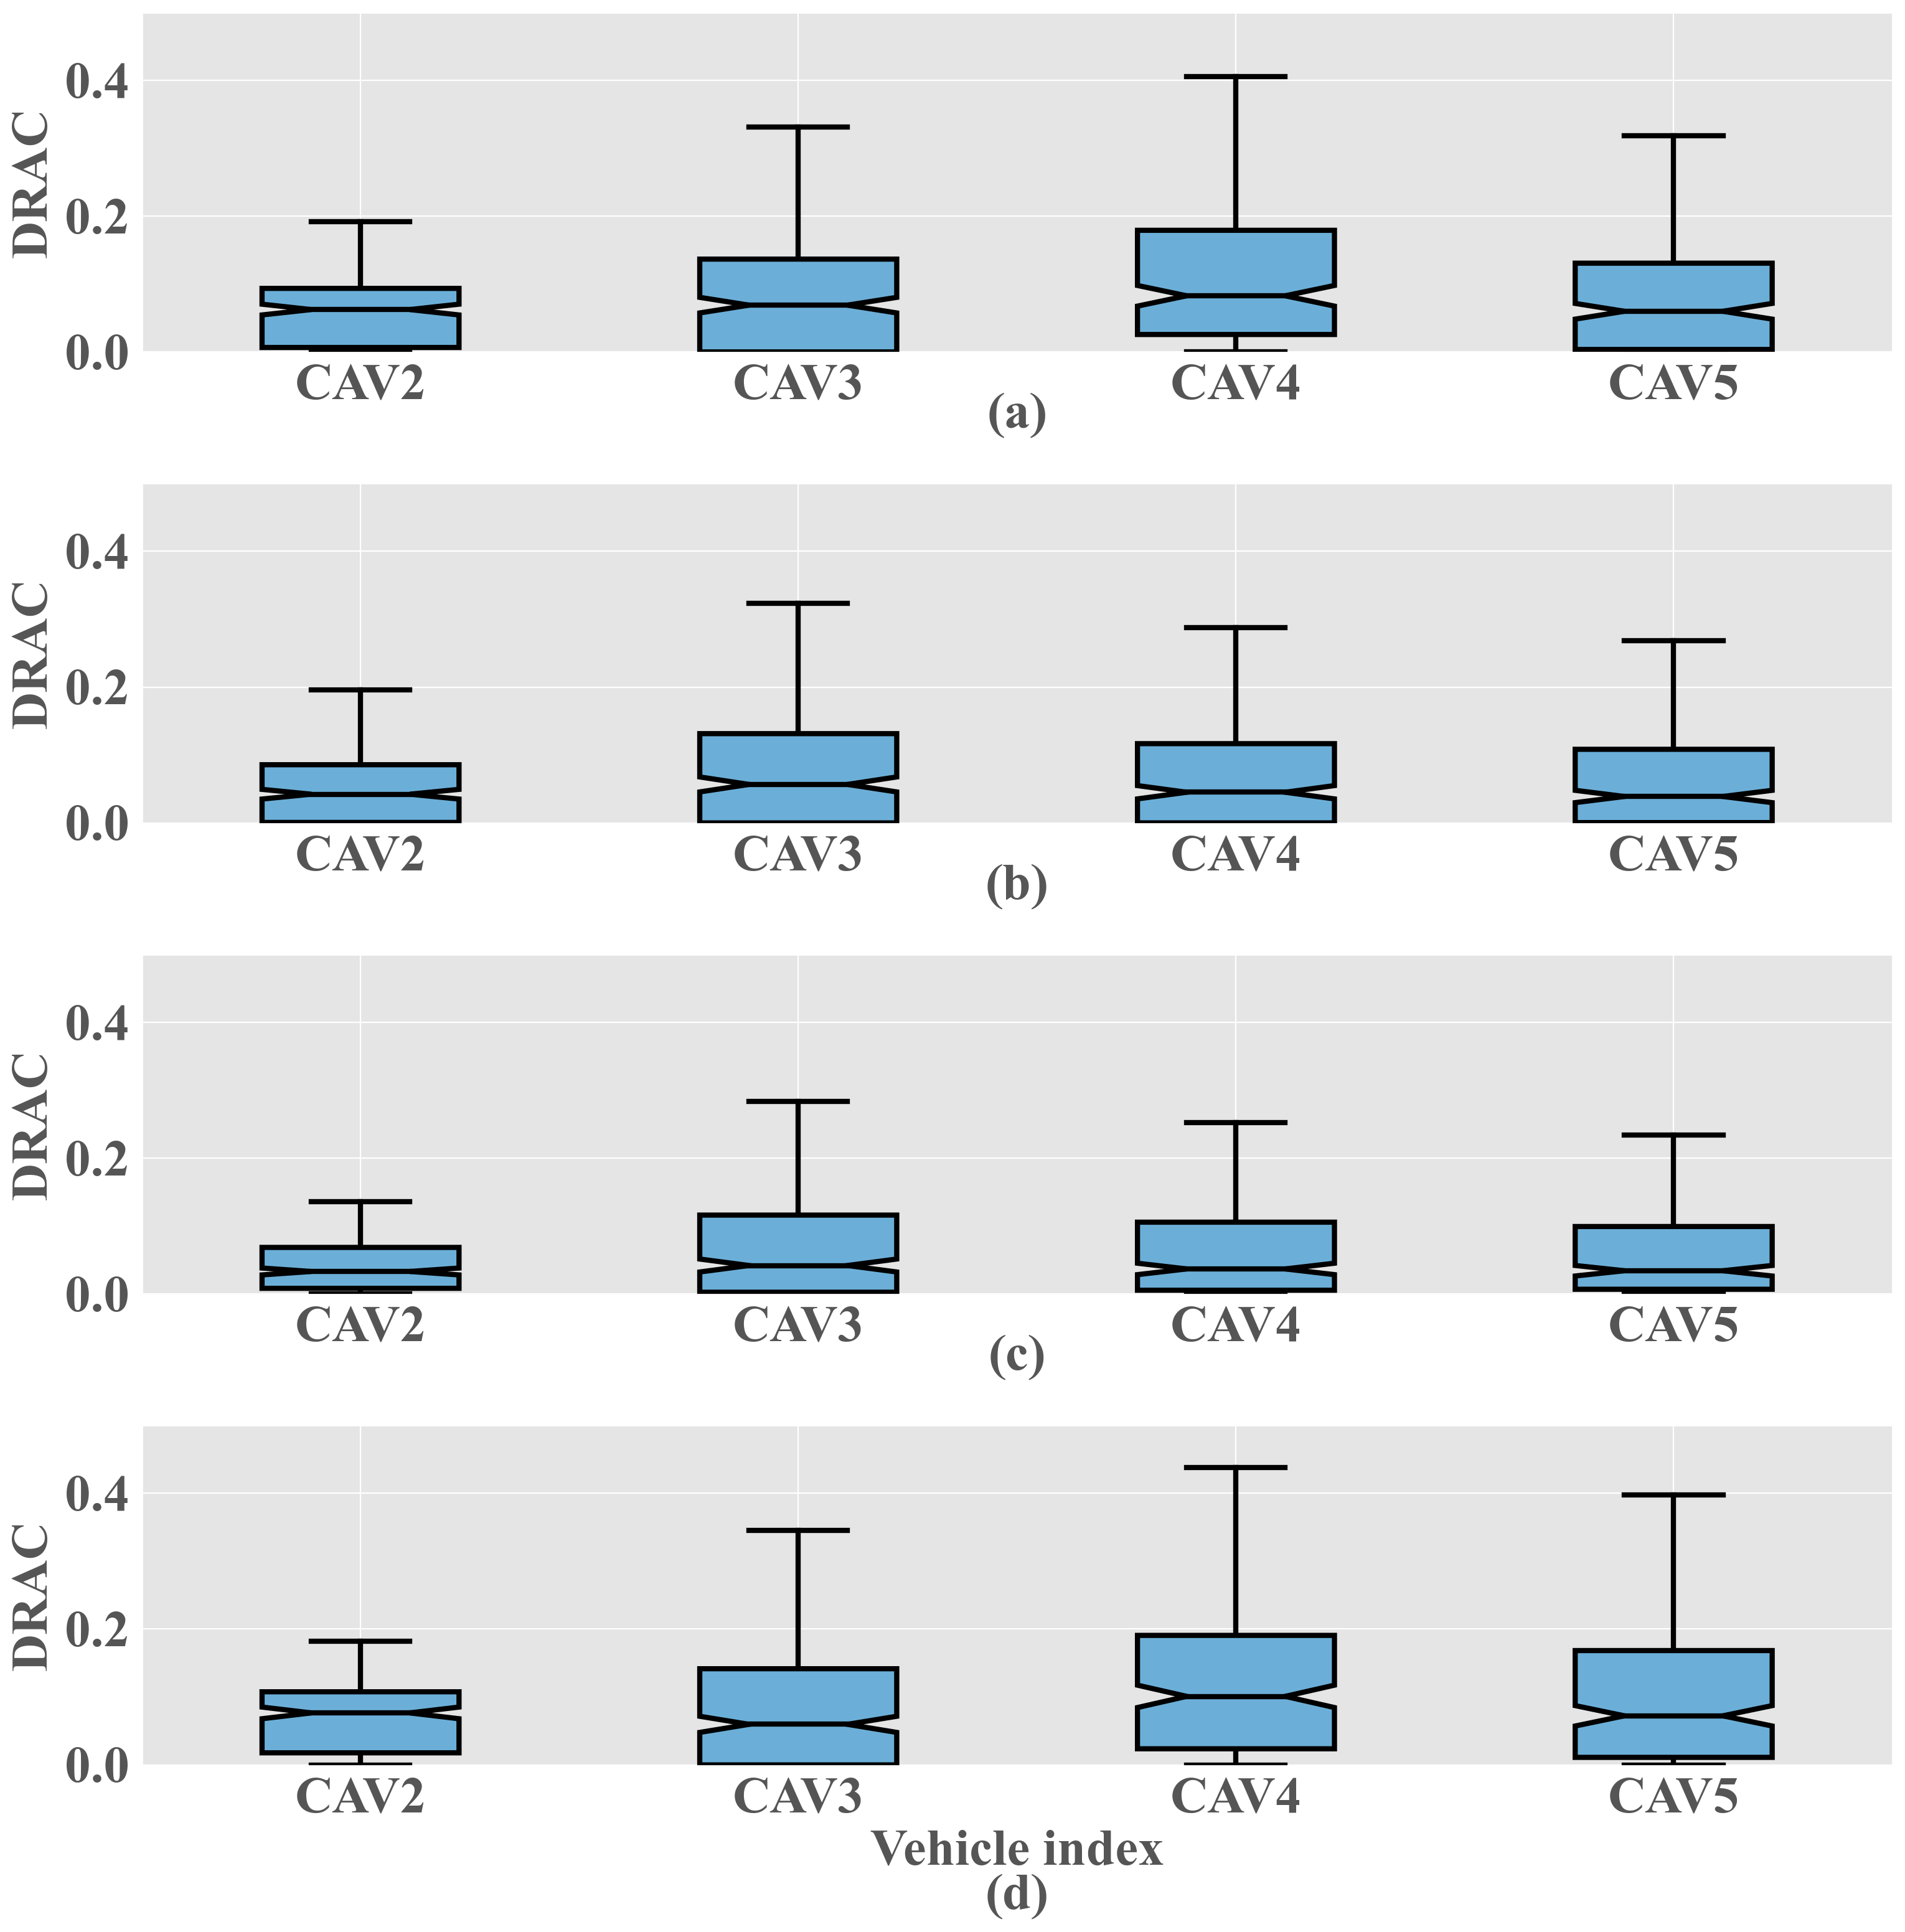
\includegraphics[width=8.5cm]{figs/fig8.png}
  \caption{~The DRAC boxplots for each CAV of each feedback control gain under investigation: (a) Parameter \uppercase\expandafter{\romannumeral1}; (b) Parameter \uppercase\expandafter{\romannumeral2}; (c) Parameter \uppercase\expandafter{\romannumeral3}; (d) Parameter \uppercase\expandafter{\romannumeral4}.}
  \label{fig8}
\end{figure}



From Fig.\ref{fig8}, a notable phenomenon can be observed by comparing the boxplots. The median DRAC of all CAVs under Parameter \uppercase\expandafter{\romannumeral2} and Parameter \uppercase\expandafter{\romannumeral3} is significantly lower than that under Parameter \uppercase\expandafter{\romannumeral1} and Parameter \uppercase\expandafter{\romannumeral4}, which is consistent with the rough results obtained in the tracking performance analyses. This finding suggests that increasing the gain of spacing and velocity errors can maintain better safety compared to increasing the gain of acceleration error. Furthermore, a second conclusion can be drawn by comparing different CAVs under the same feedback control gain. Despite the control parameters being identical, the position of a CAV in the platoon influences the safety conditions.

\subsection{Numerical analyses of the alternative IFTs}
\label{Section 5.3}

In this subsection, the parameters in Table~\ref{table1} are still adopted for both network and traffic simulation. Moreover, the control parameters are set to ${k_i} = {[0.3,0.3,0.3]^T}$ and ${h_i} = 0.6s $. The difference is that the section mainly analyzes the tracking performance of the CAV platoon employed by PF, BD or BDL. It is worth mentioning that the control parameters chosen here still exist matrixes $P,S,Q,R,$ and $X$ satisfy the Theorem~\ref{theorem6}, which can be found in Appendix C.

As in Section~\ref{Section 5.2.1}, the Trapezoidal signal defined in Section~\ref{Section 5.1} is employed to investigate the tracking performance of different IFTs. The tracking performance of the CAV platoon is presented in Fig.\ref{fig9}.


\begin{figure}

  \centering
  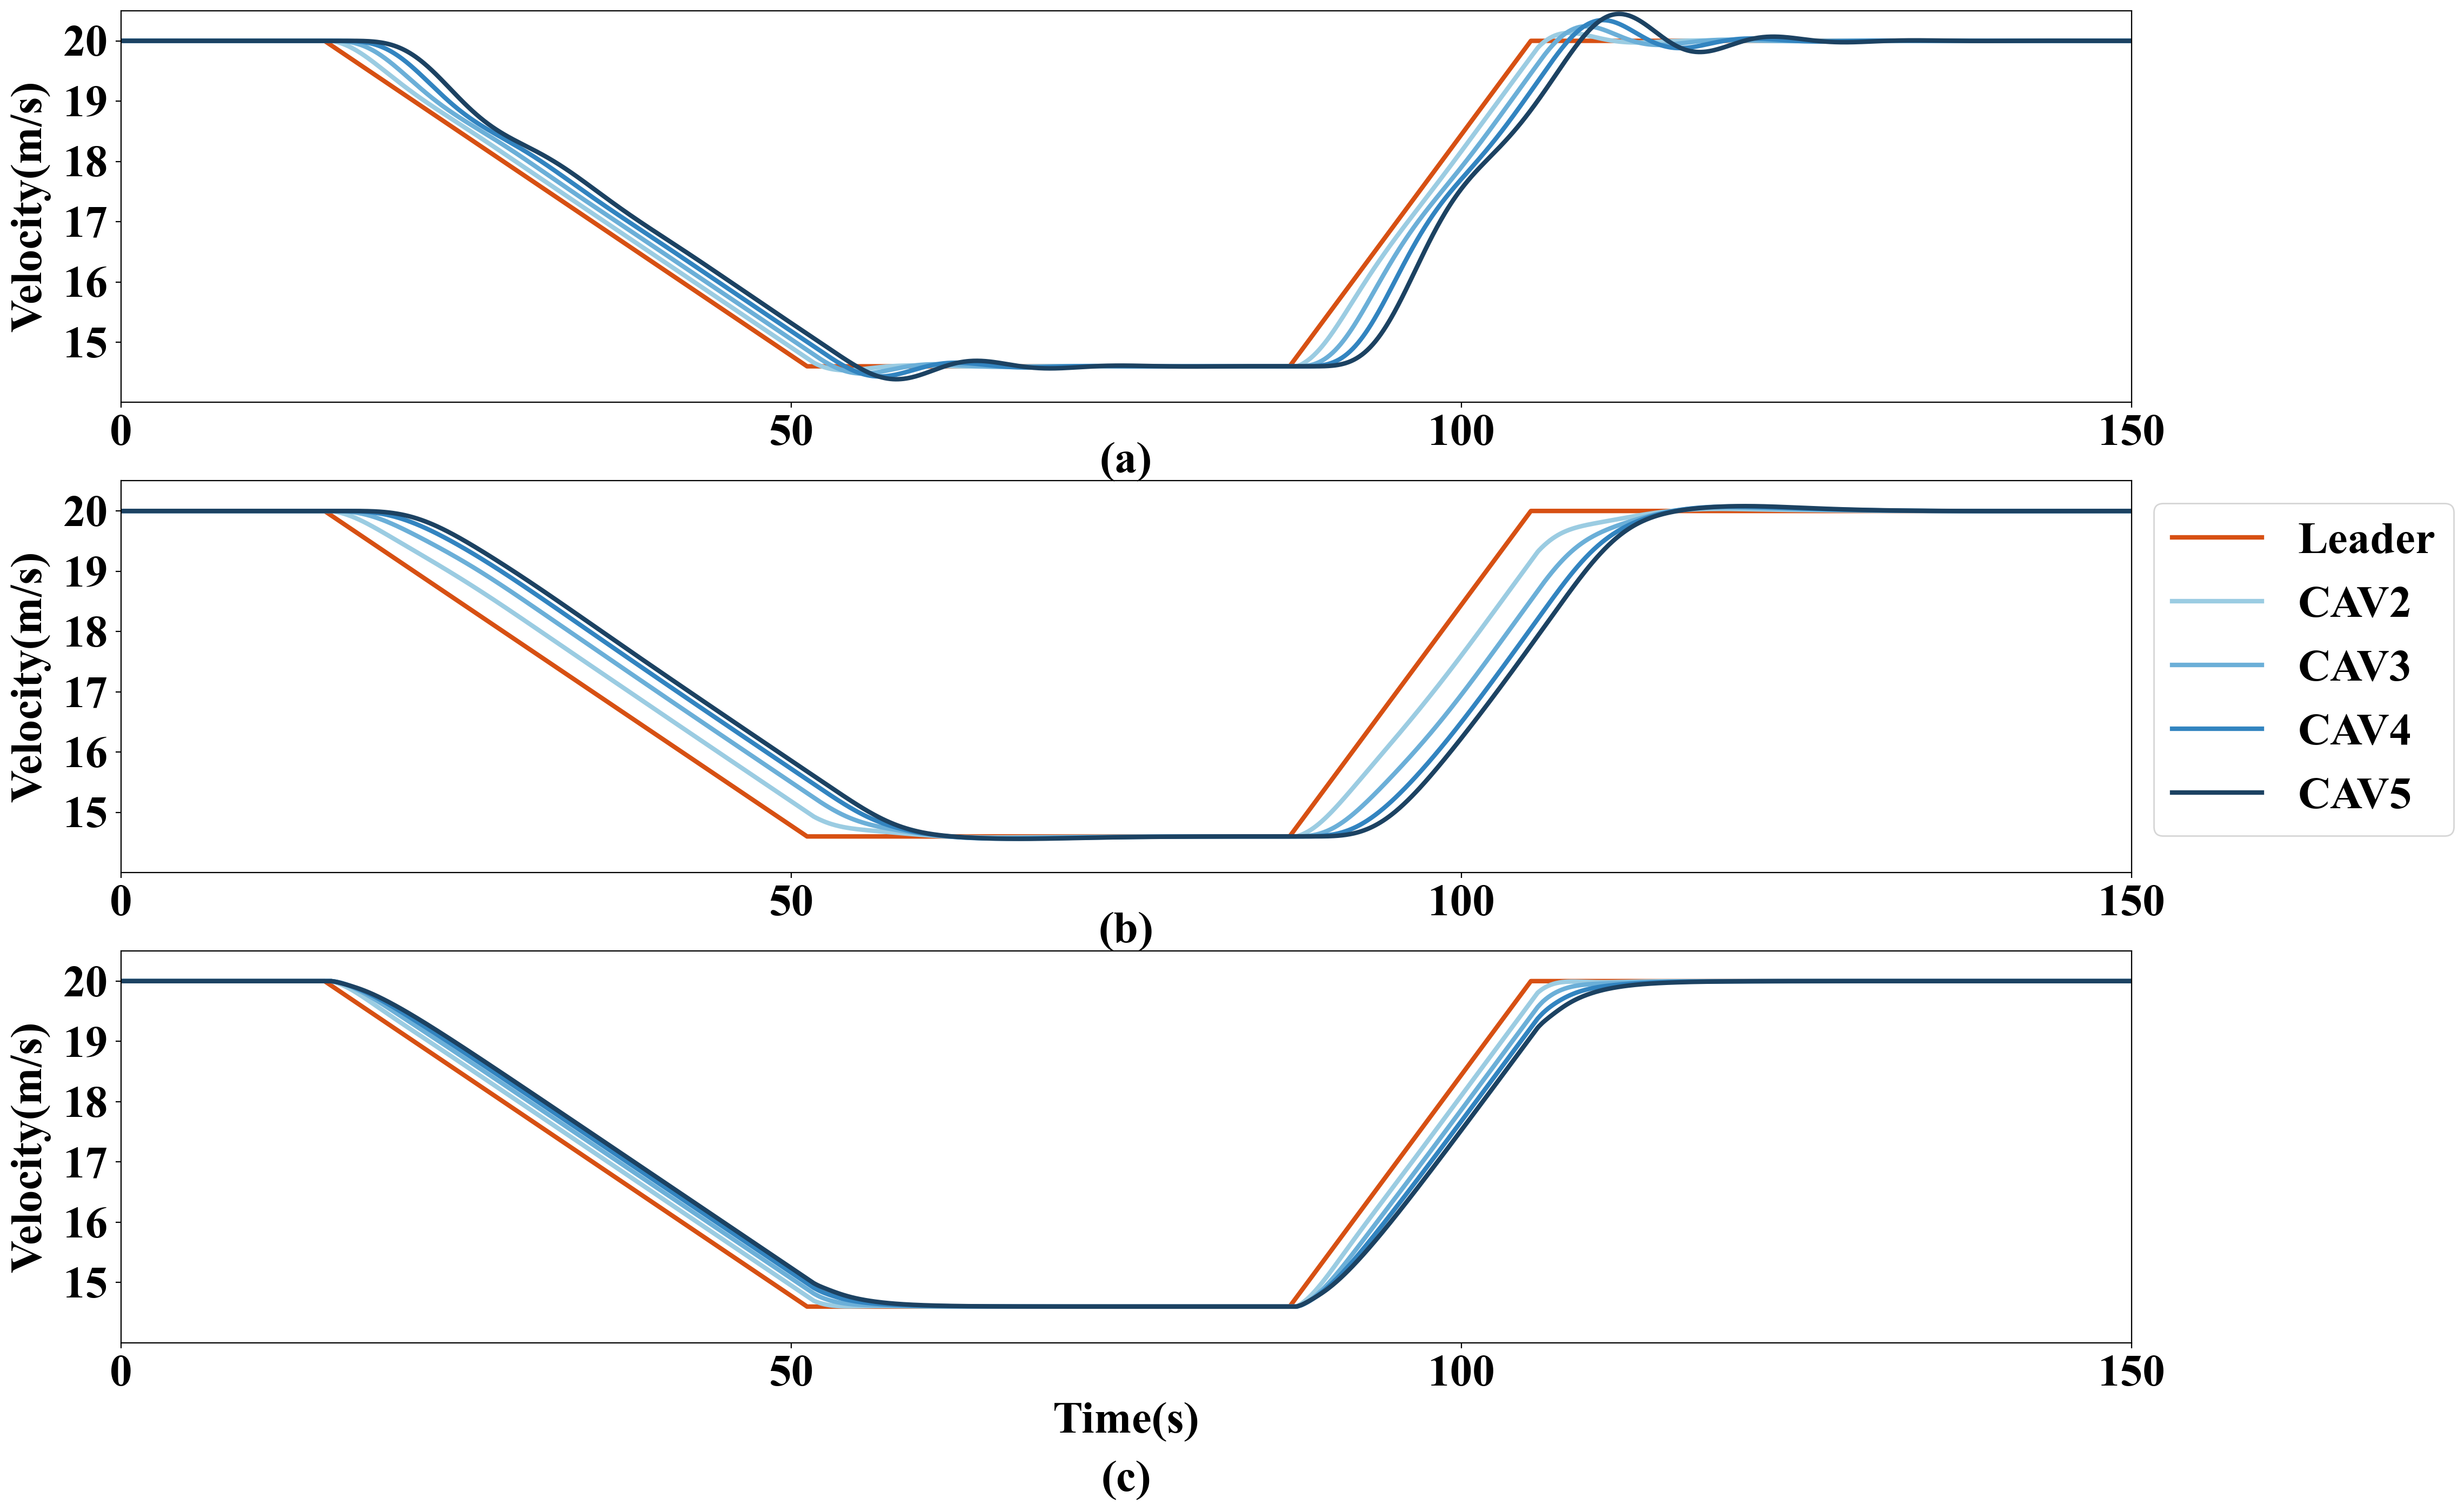
\includegraphics[width=8.5cm]{figs/fig9.png}
  \caption{~Tracking performance of the CAV platoon for the Trapezoidal signal in Fig. 3(a,b) under the alternative three IFTs: (a) presents tracking results under PF; (b) presents tracking results under BD; (c) denotes the case under BDL.}
  \label{fig9}
\end{figure}


Alternative IFTs have also been evaluated, and they have demonstrated favorable tracking performance. A similar phenomenon can be observed, where the transient response from tracking Leader motion decreases gradually, thanks to stability. It is worth noting that for the cases of BD and BDL, the tracking process is smooth; on the contrary, there are significant fluctuations in the tracking process for the case of PF, as disclosed in the recent technical literature \citep{Zheng2015}.

\begin{figure}

  \centering
  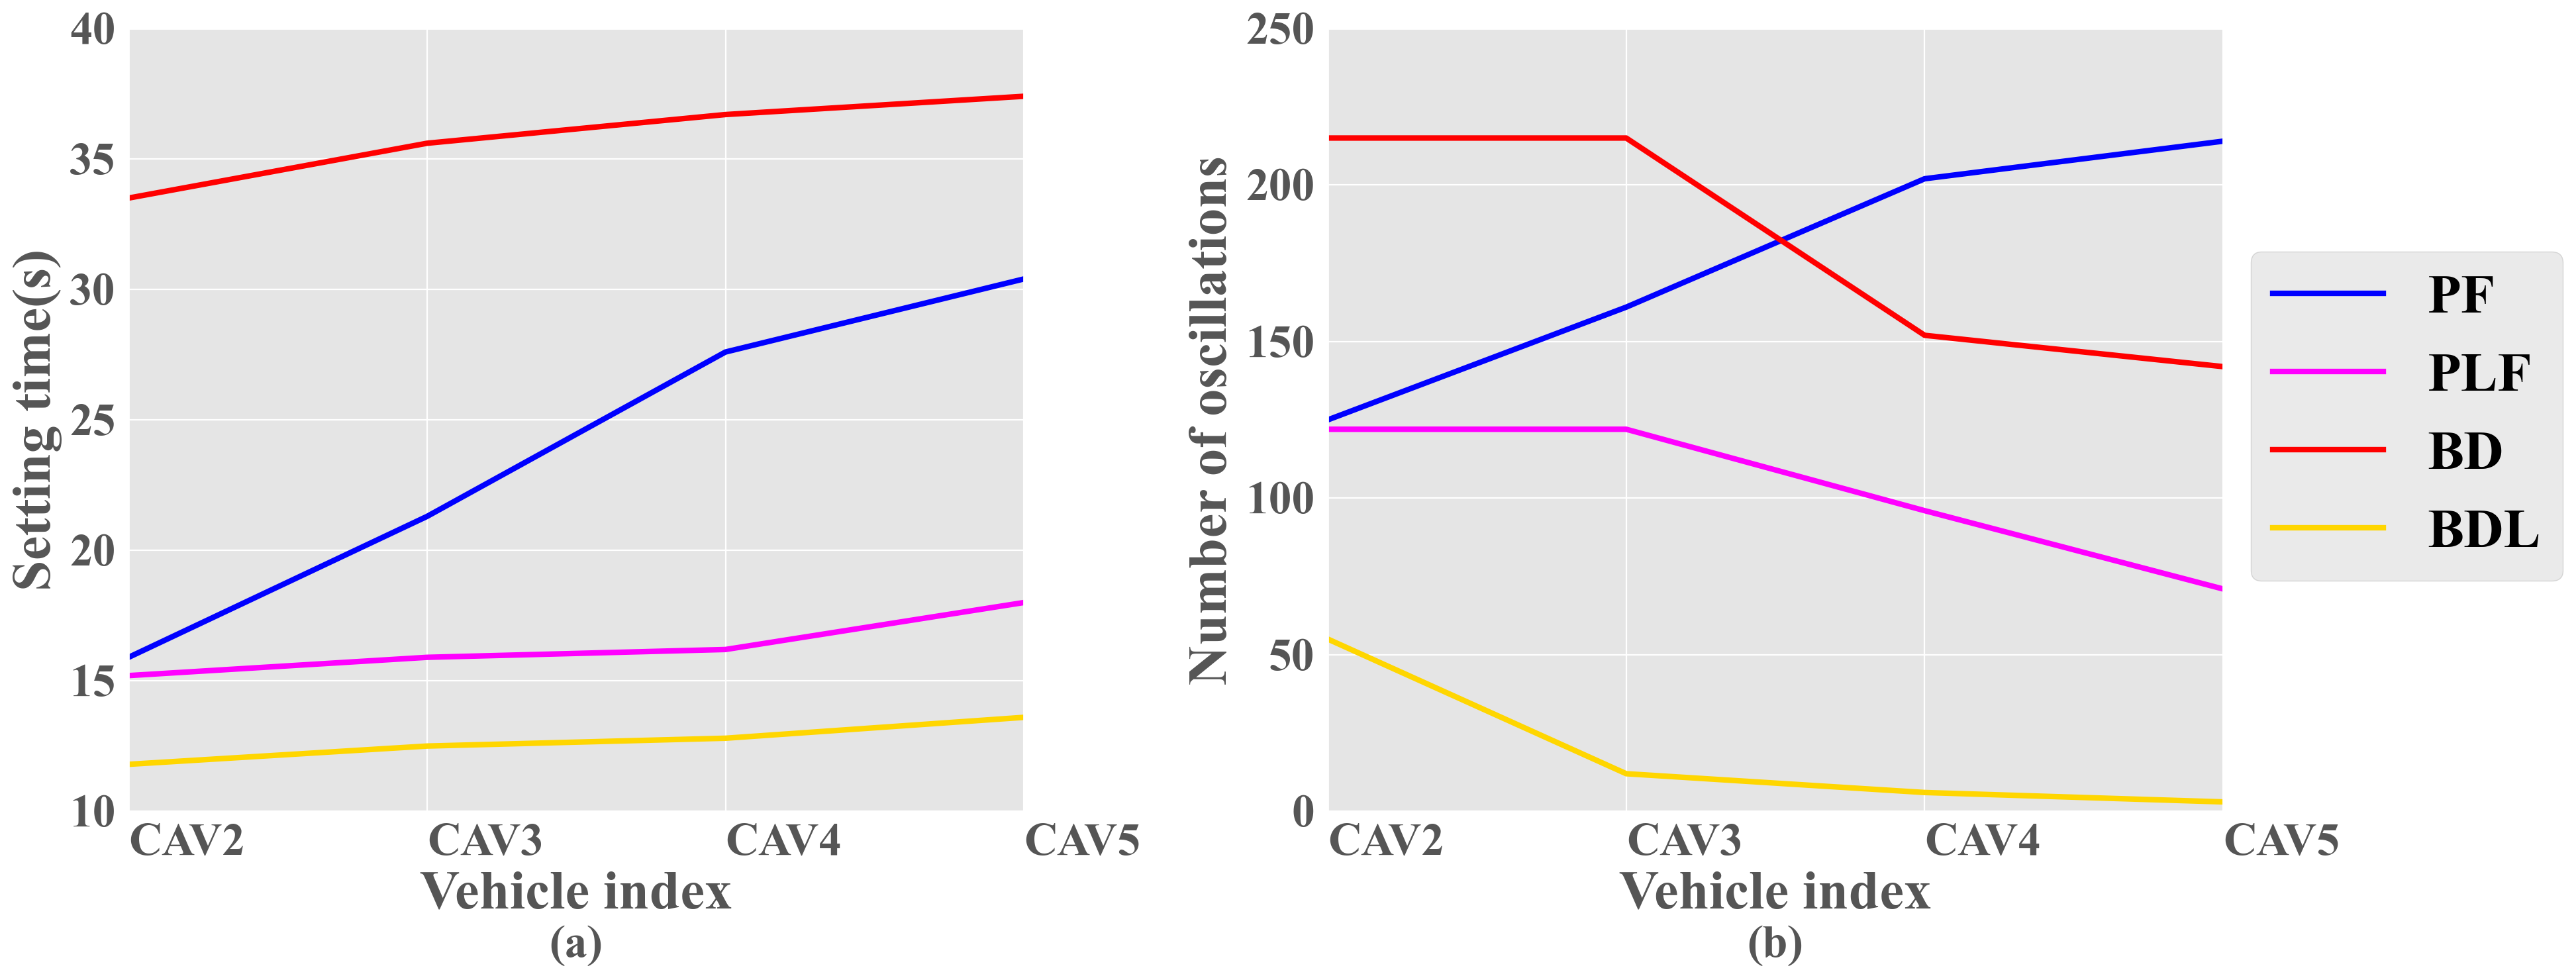
\includegraphics[width=8.5cm]{figs/fig10.png}
  \caption{~Indicators for evaluating the transient response of each CAV among the CAV platoon under the four IFTs: (a) the case of setting time; (b) the case of the number of oscillations.}
  \label{fig10}
\end{figure}

Similarly, ST and NOO are analyzed to investigate the specific effects of different IFTs on the transient response, and the results are demonstrated in Fig.\ref{fig10}. It can be found that the case under BD has a significantly higher ST than the cases under the other three IFTs. Moreover, although the ST of the cases under all IFTs increases with the increase of the vehicle index, only the case under PF increases significantly while the cases under the other IFTs increase very slightly. One conclusion can be drawn that the CAV platoon with PLF and BDL recovers from the perturbation to the equilibrium state more quickly than PF and BD. In fact, this phenomenon arises due to the direct communication with the leader, which effectively mitigates hard oscillations during transients.


On the other hand, as the vehicle index increases, for the cases under PLF, BD, and BDL, the NOO decreases, while for the cases under PF, the NOO increases. Furthermore, of the other three IFTs, the case under BD has the largest NOO, and the case under BDL has the smallest. In general, the transient performance can be significantly enhanced by communicating with the leader and bi-directional communication.



\section{Conclusion and future work}
\label{Section 6}

In this paper, we propose a general supermatrix modeling approach for the CAV platoon, taking into account time-varying communication delays. Communication relationships within a CAV platoon, typically defined by IFT, are described using graph theory. The linear time-invariant state time-varying delay system corresponding to the CAV platoon employing a CTH control strategy is modeled using supermatrices. By applying the Wirtinger-Based Integral Inequality and Lyapunov-Krasovskii Stability Theorem, a novel stability condition for the general CAV platoon is derived, based on the properties of the linear time-invariant state time-varying delay system. Moreover, extensive numerical analyses are conducted to thoroughly assess the tracking performance and safety conditions of four control parameters, offering guidance for selecting control parameters. Finally, we present a comparison of tracking performance between CAV platoons employing different IFTs, providing insights into IFT selection.

The theoretical and numerical analysis leads us to the following conclusions:
\begin{enumerate}
\item A stability condition considering time-varying delay for the CAV platoon can be obtained using the Lyapunov-Krasovskii Stability Theorem and Wirtinger-Based Integral Inequality.
\item The CAV platoon, using the investigated control parameters and IFTs, can smoothly track leader motion, maintain safe conditions in various scenarios, and ensure stability.
\item Both tracking performance and safety conditions benefit from increasing the gain of spacing and velocity errors, while increasing the gain of acceleration errors does not.
\item Communication with the leader and bi-directional communication can significantly enhance tracking and transient performance from an IFT perspective.
\end{enumerate}

However, we recognize that the vehicle behavior in the simulation is a simplification of reality, and additional field experiments are required to provide a more accurate analysis of tracking performance. Similarly, the time-varying delay function used in this paper, an assumed Bessel function that satisfies the condition of both the delay and its derivative being bounded, does not perfectly fit the actual time-varying delay. Hence, corresponding field experiments should be conducted to gain insights into the time-varying relationship of communication delays. Furthermore, future research should focus on investigating the control parameter scheme yielding optimal tracking performance through theoretical research and field experiments and designing novel control strategies to enable smoother and safer tracking performance.

\appendix


\section*{Appendix A.~Feedback control for linearization}
\label{AppendixA}
In this appendix, we provide the linearization of the longitudinal vehicle dynamic in Equation (\ref{eq1}). The functions of the lumped uncertain resistance forces, including $f_i^g(t)$, $f_i^w(t)$, and $f_i^r(t)$ are expressed as follows:
\begin{equation}
  \left\{\begin{array}{l}
    f_{i}^{g}(t)=m_{i} g \sin \left(\theta_{i}(t)\right),                        \\
    f_{i}^{w}(t)=\frac{1}{2} \rho C_{D} A_{F}\left(v_{i}(t)+v_{w}(t)\right)^{2}, \\
    f_{i}^{r}(t)=\mu_{R} m_{i} g \cos \left(\theta_{i}(t)\right).
  \end{array}\right.
  \label{eqapp5}
\end{equation}
where $g=9.81m/s^2$ denotes the acceleration of gravity; $\theta_i(t)$ is the inclination angle of the road; $\rho$ denotes the air density; $C_D$ is the aerodynamic drag coefficient; $A_F$ represents the maximal cross-sectional/frontal area of the vehicle; $v_w(t)$ denotes the uncertain headwind speed; $\mu_R$ is the coefficient of rolling resistance.

The desired engine dynamic is modeled as follows:
\begin{equation}
  (\tau_is+1)F_i^e=U_i.
  \label{eqapp6}
\end{equation}

Adopting the inverse Laplace transformation on Equation (\ref{eqapp6}) arrives at:
\begin{equation}
  \dot{f_i^e}\left(t\right)=\frac{u_i(t)}{\tau_i}-\frac{f_i^e\left(t\right)}{\tau_i}.
  \label{eqapp7}
\end{equation}

Substituting Equation (\ref{eq1}) into Equation (\ref{eqapp7}) and differentiating both sides of Equation (\ref{eqapp7}) with respect to time, we get:
\begin{small}
\begin{equation}
  \begin{aligned}
    \dot{a}_{l}(t) & =\frac{\dot{f}_{l}^{e}(t)}{m_{i}}-\frac{\dot{f}_{l}^{g}(t)}{m_{i}}-\frac{f_{l}^{i \omega}(t)}{m_{i}}-\frac{\dot{f}_{l}^{r}(t)}{m_{i}}                                                                                         \\
                   & =               \frac{u_{i}(t)}{m_{i} \tau_{i}}                                                                                                                                                                               \\
                   & -               \frac{a_{i}(t)+\mathrm{g} \sin \left(\theta_{i}(t)\right)\left[1-\tau_{i} \mu_{R} \dot{\theta}_{l}(t)\right]+\mathrm{g} \cos \left(\theta_{i}(t)\right)\left[1+\tau_{i} \dot{\theta}_{l}(t)\right]}{\tau_{i}} \\
                   & -               \frac{\frac{1}{2} \rho C_{D} A_{F}\left(v_{i}(t)+v_{w}(t)\right)\left(\left(v_{i}(t)+v_{w}(t)\right)+2 \tau_{i}\left(a_{i}(t)+\dot{v}_{w}(t)\right)\right)}{\tau_{i}}.
  \end{aligned}
  \label{eqapp8}
\end{equation}
\end{small}

Thus, the nonlinear state feedback chosen for linearizing can be defined by:
\begin{equation}
  \begin{aligned}
    u_i^\ast\left(t\right)= & m_iu_i\left(t\right)+g\sin{\left(\theta_i\left(t\right)\right)}\left[1-\tau_i\mu_R\dot{\theta_i}\left(t\right)\right]\\
    &+g\cos{\left(\theta_i\left(t\right)\right)}\left[1+\tau_i\dot{\theta_i}\left(t\right)\right]\ \\
                            & +\frac{1}{2}\rho C_DA_F\left(v_i\left(t\right)+v_w\left(t\right)\right)\\
                            &\quad \left(\left(v_i\left(t\right)+v_w\left(t\right)\right)+2\tau_i(a_i\left(t\right)+\dot{v_w}\left(t\right))\right).
  \end{aligned}
  \label{eqapp9}
\end{equation}

Under the new feedback control input, the Equation (\ref{eq1}) can be rewritten as:
\begin{equation}
  \tau_i\dot{a_i}\left(t\right)+a_i\left(t\right)=u_i(t).
  \label{eqapp10}
\end{equation}


\section*{Appendix B.~Connection between Lyapunov-Krasovskii Stability Theorem and Second Lyapunov method.}
\label{AppendixCCC}
First, we present a lemma on the Lyapunov function:
\begin{lemma}
  \label{lemmaYY}
  (\citep{Kolmanovskii1999}) Let a system $\dot{X}(t)=f(X(t), X(t-h\left(t\right)))$ with $f\left(0,0 \right)= 0$. Assume the Lyapunov function $F:G\rightarrow\mathbb{R}$ exists with $X,y\in G$, $F\left(y\right)<F\left(X\right)$ implies
  \begin{equation}
    \left(\dot{F}\left(X\right)f\left(X,y\right)\right)\left(\ddot{F}\left(X\right)f\left(X,y\right)\right)\le0.
  \end{equation}

  Then the solution $X(t)\equiv0$ is stable.
\end{lemma}

Suppose there exists a Lyapunov function $F:\mathbb{R}^n\rightarrow\mathbb{R}$. Then define functional $V:\mathcal{C}\rightarrow\mathbb{R}$ as follows:
\begin{equation}
  V(\phi ): = \mathop {\max }\limits_{ - h \le \theta  \le 0} F(\phi (\theta )),(\forall \phi  \in \mathcal{C}).
  \label{yy1}
\end{equation}

By definition, the following conditions hold:
\begin{small}
\begin{equation}
  \dot{V}(\phi)\left\{\begin{array}{cl}
    \leq 0,                                                          & \text { if } F(\phi(0))<V(\phi), \\
    =\max \left(\dot{F}(\phi(0)), f(\phi(0), \phi(-h(t))), 0\right), & \text { if } F(\phi(0))=V(\phi),
  \end{array}\right.
\end{equation}
\end{small}
where $f(\phi(0), \phi(-h(t)))=\Psi\phi(0)+\Psi_d\phi(-h(t))$.

Thus $\dot{V}\left(\phi\right)>0$ holds if and only if the following condition holds:
\begin{equation}
  F(\phi (0)) = \mathop {\max }\limits_{ - h \le \theta  \le 0} F(\phi (\theta ))\;and(\dot F(\phi (0)),f(\phi(0), \phi(-h(t)))) > 0.
  \label{yy3}
\end{equation}

The function $F$ can be defined in some neighborhood $G\subset\mathbb{R}^n$. And the functional $V$ is then defined for $\phi\in\mathcal{C}$ with values in $G$.

Suppose Equation~(\ref{yy3}) holds for some functions $\phi\in\mathcal{C}$, then we can obtain the inequality $F\left(\phi\left(-h\left(t\right)\right)\right)<F\left(\phi\left(0\right)\right)$ making $\phi$ arbitrarily small. Thus the second condition in Equation~(\ref{yy3}) still holds, but conflicts with Lemma~\ref{lemmaYY}. Therefore $\dot{V}\left(\phi\right)\le0$ holds constantly for all $\phi$.

It can be concluded that the Lyapunov-Krasovskii Stability Theorem can be considered as an extension of the Second Lyapunov method to functional space. This extension does not introduce any additional constraints since it only constrains the definite sign at the start and end points instead of in the neighborhood. As a result, the stability conditions obtained using the Lyapunov-Krasovskii Stability Theorem are more accurate than those obtained using the Second Lyapunov method. This conclusion has been supported by previous research \citep{wang2016fuzzy,lian2020dissipativity}.


\section*{Appendix C.~Attachments uploaded to GitHub}
\label{AppendixB}
The uploaded code for this paper includes the formulation of Theorem~\ref{theorem3} and the construction of LMIs for Theorem~\ref{theorem6}. Additionally, matrices corresponding to the four sets of control parameters for PLF, as selected in Section~\ref{Section 5.2}, and three sets for PF, BD, and BDL, as selected in Section~\ref{Section 5.3}, which are compatible with Theorem~\ref{theorem6}, have been included in the repository. The file repository URL is: https://github.com/ruantiancheng/code-of-paper8.
% \afterpage{\clearpage}


% use section* for acknowledgment
\section*{Acknowledgment}


This research was sponsored by the National Key Research and Development Program of China (No. 2022ZD0115600),
 National Science Foundation of China (No. 52072067), Postgraduate Research \& Practice Innovation Program of Jiangsu Province (KYCX22\_0266), and Natural Science Foundation of Jiangsu Province (No. BK20210249).


% Can use something like this to put references on a page
% by themselves when using endfloat and the captionsoff option.
\ifCLASSOPTIONcaptionsoff
 \newpage
\fi



% trigger a \newpage just before the given reference
% number - used to balance the columns on the last page
% adjust value as needed - may need to be readjusted if
% the document is modified later
%\IEEEtriggeratref{8}
% The "triggered" command can be changed if desired:
%\IEEEtriggercmd{\enlargethispage{-5in}}

% references section
% can use a bibliography generated by BibTeX as a .bbl file
% BibTeX documentation can be easily obtained at:
% http://mirror.ctan.org/biblio/bibtex/contrib/doc/
% The IEEEtran BibTeX style support page is at:
% http://www.michaelshell.org/tex/ieeetran/bibtex/
\bibliographystyle{IEEEtran}
% argument is your BibTeX string definitions and bibliography database(s)
%\bibliography{IEEEabrv,../bib/paper}
%\bibliography{cas-refs}
% <OR> manually copy in the resultant .bbl file
% set second argument of \begin to the number of references
% (used to reserve space for the reference number labels box)

\bibliography{cas-refs}


% that's all folks
\end{document}


